\documentclass[a4paper,10pt,titlepage]{report}
%%This template is based on Paco van Beckhoven's thesis.

\usepackage{xspace}
\usepackage{xargs}   % Use more than one optional parameter in a new commands
\usepackage[pdftex,dvipsnames]{xcolor}

% Putting images next to each other
\usepackage[font=bf,]{caption}
\usepackage{subcaption}
\input{glyphtounicode}

% for last page
\usepackage{lastpage}

\usepackage[english]{babel}
\usepackage[utf8]{inputenc}
\usepackage{csquotes}
\usepackage[margin=1in]{geometry}
\usepackage{fancyhdr}
\usepackage{booktabs}
\usepackage{paralist}
\usepackage{graphicx}
\usepackage{tabularx}
\usepackage{adjustbox}
\usepackage{titlepic}
\usepackage{vhistory}
\usepackage{enumitem}
\usepackage{longtable}
\usepackage[backend=biber, style=ieee,citestyle=numeric-comp]{biblatex}
\usepackage[colorinlistoftodos, prependcaption]{todonotes}
\usepackage{placeins}
\usepackage{multirow}
\usepackage{amsmath,amssymb}
\usepackage[hidelinks]{hyperref}
\usepackage[acronym,nogroupskip,nohypertypes={acronym},toc,section=chapter]{glossaries}
\usepackage{amssymb}
\usepackage{verbatim}
\usepackage{cmap}
\usepackage{xparse}

\usepackage{sectsty}
\sectionfont{\LARGE}
\subsectionfont{\Large}
\subsubsectionfont{\large}

%\usepackage[ansinew]{inputenc}
%\usepackage[T1]{fontenc}
%\usepackage{libertine}
\input{glyphtounicode}

\pdfglyphtounicode{f_f}{FB00}
\pdfglyphtounicode{f_f_i}{FB03}
\pdfglyphtounicode{f_f_l}{FB04}
\pdfglyphtounicode{f_i}{FB01}

\pdfgentounicode=1



%Appendix package + appendix in chapter title
\usepackage[titletoc]{appendix}




%for highlighting findings
\usepackage{tcolorbox}

% for highlighting code examples
\usepackage{listings}

\newcommand{\ie}{\emph{i.e.},\xspace}
\newcommand{\eg}{\emph{e.g.},\xspace}
\newcommand{\etc}{\emph{etc.}\xspace}
\newcommand{\etal}{\emph{et al.}\xspace}

\newcommand{\sig}{\gls{sig}}
\newcommand{\sigs}{\glspl{sig}}

\newcommandx{\unsure}[2][1=]{\todo[linecolor=red,backgroundcolor=red!25,bordercolor=red,#1, inline]{#2}}
\newcommandx{\discussion}[2][1=]{\todo[linecolor=red,backgroundcolor=green!25,bordercolor=red,inline,#1]{#2}}

\newcommandx{\improvement}[2][1=]{\todo[linecolor=blue,backgroundcolor=blue!25,bordercolor=blue,#1]{#2}}

\newcommandx{\reminder}[2][1=]{\todo[linecolor=yellow,backgroundcolor=yellow!25,bordercolor=yellow,#1]{#2}}

\newcommandx{\lessprio}[2][1=]{\todo[linecolor=Plum,backgroundcolor=Plum!25,bordercolor=Plum,#1]{#2}}
\newcommandx{\todocontent}[2][1=]{\todo[author=\textbf{Planned content},backgroundcolor=Goldenrod!25,bordercolor=Goldenrod,inline,#1]{#2}}


%%Some additional table column specifiers, allowing for fixed width columns that wrap.
\newcolumntype{L}[1]{>{\raggedright\let\newline\\\arraybackslash\hspace{0pt}}p{#1}}
\newcolumntype{C}[1]{>{\centering\let\newline\\\arraybackslash\hspace{0pt}}p{#1}}
\newcolumntype{R}[1]{>{\raggedleft\let\newline\\\arraybackslash\hspace{0pt}}p{#1}}

\definecolor{ryel}{HTML}{fcd116}
\definecolor{rred}{HTML}{ce1126}
\definecolor{rblu}{HTML}{0a3eb9}
%these are examples of commands that may facilitate feedback annotations in the document
%replace \paco by your name and \ana by your supervisor's name
%\newcommandx{\ana}[2][1=]{\todo[linecolor=rblu,backgroundcolor=ryel,bordercolor=rred,#1]{#2}}
%\newcommandx{\paco}[2][1=]{\todo[author=Paco,linecolor=blue,backgroundcolor=white,bordercolor=red,#1]{#2}}

%\usepackage[htt]{hyphenat}
\allowdisplaybreaks[1]
\definecolor{lstgrey}{rgb}{0.95,0.95,0.95}
\usepackage{listings}
\lstset{
    language=Java,
    frame=single,
    backgroundcolor=\color{lstgrey},
    basicstyle=\small\ttfamily,
    captionpos=b,
    tabsize=2,
    commentstyle=\color{gray},              % Comments font
    numbers=left,                           % Line nums position
    numberstyle=\tiny,                      % Line-numbers fonts
    % stepnumber=1,                           % Step between two line-numbers
    % numbersep=5pt,                          % How far are line-numbers from code
    tabsize=2,                              % Default tab size
    captionpos=b,                           % Caption-position = bottom
    breaklines=true,                        % Automatic line breaking?
    breakatwhitespace=false,                % Automatic breaks only at whitespace?
    showspaces=false,                       % Dont make spaces visible
    showtabs=false,                         % Dont make tabls visible
    columns=flexible,                       % Column format
}

\NewDocumentCommand{\rot}{O{90} O{1em} m}{\makebox[#2][l]{\rotatebox{#1}{#3}}}

\newcommand{\cn}[1]{\textsuperscript{\color{red} ~[citation needed]#1~}}

\newcommand{\blankl}{\bigskip\noindent}
\newcommand{\blankls}{\smallskip\noindent}

% -- title page is a modified version of https://github.com/software-engineering-amsterdam/latex/blob/master/thesis/uvamscse.cls
\newcommand{\email}[1]{\ttfamily\href{mailto:#1}{#1}}

\newcommand{\uvacoverfoot}{%
	\vfill
	\begin{center}
		\begin{tabular}{r|l}
			\multirow{3}{*}{
\includegraphics[height=48pt]{uva.pdf}}
			&\textsc{\Large Universiteit van Amsterdam}\\
			&\textsc{Faculteit der Natuurwetenschappen, Wiskunde en Informatica}\\
			&\textsc{Master Software Engineering}\\
			&\url{http://www.software-engineering-amsterdam.nl}
		\end{tabular}
	\end{center}
}

\renewcommand{\maketitle}{%
	% The cover page
	% --------------
	\thispagestyle{empty}
	\enlargethispage{30pt}
	\renewcommand{\thefootnote}{\fnsymbol{footnote}}
	% Will be page 0, s.t. contents start on page 1
	\setcounter{page}{0}
	% \eccoverhead
	% Volume and article title, author(s)
	\vspace{60pt}
	\begin{center}
		{\Huge\bfseries Measuring the degree of library dependency \par}

		\vspace{44pt}
		{\Large\bfseries Núria Bruch Tàrrega \par}
		\email{nuria.bruch@gmail.com}\\
		\vspace{11pt}
		July 16, 2020, \pageref{LastPage} pages
	\end{center}
	\vfill
	\begin{tabular}{ll}
		\textbf{Academic supervisor:} 	& Dr. Ana M. Oprescu, \email{ana.oprescu@uva.nl} \\
		\textbf{Host supervisor:} & Dr. Lodewijk Bergmans, \email{l.bergmans@sig.eu}\\
		\textbf{Host supervisor:} & Dr. Miroslav \v{Z}ivkovi\'{c},  \email{m.zivkovic@sig.eu}\\
		\textbf{Host organisation:} & Software Improvement Group (SIG), \href{https://www.softwareimprovementgroup.com}{www.softwareimprovementgroup.com} \\
	\end{tabular}
	\uvacoverfoot
	\newpage
	\setcounter{footnote}{0}
	\renewcommand{\thefootnote}{\arabic{footnote}}
	\setlength{\parskip}{0pt}
}

%\newcommand{\uvaabstract}{}latex
%\renewcommand{\abstract}[2][Abstract]{\renewcommand{\uvaabstract}{\chapter*{Abstract}%
%\par#2\newpage}}


%-------- End of ``title page''

%Fancy page headers
\pagestyle{fancy}
\fancyhf{}
\fancyhead[L]{\leftmark}
\fancyfoot[C]{\thepage}
\setlength{\headheight}{14pt}


%%FINDING ENV
\newcounter{findingctr}

\newenvironment{finding}{%      define a custom environment
	\refstepcounter{findingctr}% increment the environment's counter
	\begin{tcolorbox}
	\textbf{Finding \thefindingctr:}
}{\end{tcolorbox}}
% If you want numbers that start with the chapter or section number (e.g. 7.1.1 or 7.1) enable the following lines
%\usepackage{amsmath}
%\numberwithin{findingctr}{chapter}


% Decrease the size of all these lists
\setlist{topsep=4pt,parsep=1pt,partopsep=4pt}


\lstset{
	basicstyle=\footnotesize,        % the size of the fonts that are used for the code
	breakatwhitespace=false,         % sets if automatic breaks should only happen at whitespace
	breaklines=true,                 % sets automatic line breaking
	captionpos=b,                    % sets the caption-position to bottom
	frame=single,                    % adds a frame around the code
	language=Java,                 % the language of the code
	keywordstyle=\bf,
	tabsize=2                       % sets default tabsize to 2 spaces
}

%make it fit more nicely
\setlength\extrarowheight{2pt}

\makeglossaries
\loadglsentries[acronym]{acronym}

\addbibresource{./res.bib}

\begin{document}
\maketitle
\newpage
% !TEX root = ../main.tex
\chapter*{Abstract}
The usage of libraries, both commercial and open-source, provides the implementation of certain functionalities and is a widespread practice among developers. The usage of these libraries allows developers to avoid duplicating code by reusing it instead. However, when a developer uses a library in a software product, it creates a dependency. This dependency creates transitive dependencies with the libraries this first library uses. The dependencies created when reusing a library can also carry problems. For example, if a library has a security issue, it can be propagated to the software product, which depends on it, directly or indirectly. To deal with dependencies, developers can use package managers, which allow them to install and update the libraries they use. However, these package managers generally do a simple evaluation of the dependencies: either there is a dependency or not. Hence, a detailed evaluation of the dependencies is missing. More fine-grained information could be helpful for developers that deal with vulnerabilities, breaking changes, and deprecated dependencies.

In this thesis, we propose a model for software dependencies, which can help to provide a fine-grained evaluation. The model contains three types of metrics: coupling, coverage, and usage per class. Each type offers a different perspective of the dependency and can be used with direct and transitive dependencies. For each metric in the model, we provide a formal definition and a theoretical validation by proving the metrics' properties. We additionally implemented a proof-of-concept tool, which given a library from the \textit{Maven Central Repository}, calculates the metrics of the model for each of the dependencies using bytecode analysis. Moveover, the proof-of-concept includes a visualization of the dependency tree, including the calculated metrics.

Finally, we conducted experiments to validate the model, the implementation of the proof-of-concept, and the visualization. The experiments include interviews with 15 professional developers who evaluated the model's metrics, in terms of clarity and actionability, and the proposed visualizations included in the tool.

\tableofcontents
\newpage

% !TEX root = ../main.tex
\chapter{Introduction}\label{ch:Introduction}

\section{Problem statement}

\subsection{Context}
Currently, there are many open-source libraries available for developers to reuse the features that these libraries implement. This practice is becoming more and more popular since it allows to reuse previously developed code, and helps developers avoid implementing the same functionalities multiple times.

When a developer uses an open-source library in a project, it creates a dependency between the project and the library. This implies that a significant number of projects depend on other open-source projects, and it adds the task of managing these dependencies to the maintenance tasks of the project.  Proper maintenance of the dependencies of a project is also part of the health and security of software applications, and it is one of the problems that the field of software engineering is trying to solve \cite{kula2014visualizing}. For instance, an update of a dependency can involve changing part of the code, if the update contains breaking changes \cite{Raemaekers2017}.

The management and maintenance of the dependencies of a project is an important task. External libraries, just like any other software product, can have security vulnerabilities that may affect the projects that depend on these libraries. For example, some vulnerabilities can become security problems that can have a negative impact in terms of integrity, privacy or availability.

\blankl
Currently, developers have package managers at their disposal, to ease the task of managing the dependencies of their projects. However, the dependency management available in these package managers only evaluate if a dependency exists or not and a more detailed evaluation is missing \cite{hejderup2018prazi}. For instance, here is no way to evaluate how much a project depends on a library.

\blankl
Therefore, this thesis has the aim to create a model to evaluate the dependencies, in order to obtain information of the \textit{actual usage} of the dependencies. A set of metrics is proposed to measure the dependencies between projects and the dependencies these have. The metrics are designed to evaluate the dependencies according to two different perspectives, the code affected by the dependency, and how much of a dependency is used.

\subsection{Host organization}
This project has been carried out in collaboration with the company \textit{Software Improvement Group (SIG)}, and it is motivated by the \textit{FASTEN} project \footnote{\url{https://www.fasten-project.eu/}}. The objective of this project is to improve the quality of open-source development environments to make them more secure and reliable. For this reason, the FASTEN project aims to analyze the software library dependencies that the projects have in more detail.

\subsection{Research questions}
\discussion{Still deciding whether to use software product, or libraries, how to introduce it. Because, for the PoC I am using only libraries available in Maven, but the model is meant to be used to measure the dependencies with any type of software product}
To tackle the problems described in the previous section, we specify the following research questions:

\blankl
\textbf{RQ1:} \textit{How can we measure the degree of code dependency between two software products with a direct dependency?}

\blankls
With this question, we want to propose a set of metrics to measure a dependency from the point of view of the product that has a dependency with another product. How much is it affected by the dependency.

\begin{itemize}
  \item \textbf{RQ1.1:} \textit{What constitutes a dependency between two products?}

  First, we need to determine what creates a dependency. The type of connection between the products and how can it be measured.

  \item \textbf{RQ1.2:} \textit{Which metrics can be used to measure the dependency?}

  We propose metrics to measure the dependency described. Existing metrics are considered, as well as new ones.

  \item \textbf{RQ1.3:} \textit{How can the proposed metrics be validated?}

  There are many different approaches to validate metrics, some of which are used to carry out the validation of the proposed metrics.
\end{itemize}

\blankl
\textbf{RQ2:} \textit{How can we measure the degree of code dependency between two software products with a transitive dependency?} \unsure{I'm not sure if I should phrase this question like this, or focusing on the differences: How should the measurements of the dependencies be adapted for the case of transitive dependencies}

\blankls
Transitive dependencies involve more factors than the direct dependencies. Therefore, the metrics proposed for the direct dependencies have to be adapted for the transitive ones.

\blankl
\textbf{RQ3:} \textit{How can we mesure how much is a dependency used by a software product?}

\blankls
For this question, we look at the dependency from a different perspective. In this case, we measure how much of the dependency is being used by the software product.

\blankl
\textbf{RQ4:} \textit{How can we visualize the metrics designed to model the software dependencies?}

\blankls
We present a few visualization to see the metrics of the model. The visualizations are presented to software developers to discuss the usefulness and actionability.

\subsection{Research method}
The main research method that is going to be employed during this project is \textit{Technical Action Research} (TAR) \cite{wieringa2012technical}.
This research method is artifact-based, which means that the first step is to produce the artifact meant to be used in certain situations envisioned by the researcher. The testing of this artifact, to see if it is effective in these situations, is done through a number of iterations. First, under ideal conditions, and then changing the experiments step by step to reach a real-world situation. These iterations, in the context of this project, are going to be limited due to the existing deadlines. However, there is the option of continuing with this part of the work in the future.

\blankl
In addition, the research will also include experiments. These experiments will be conducted as the empirical part of the validation of the metrics and of the proof-of-concept implementation. Additionally, the empirical validation of the effort estimation is going to be achieved by the means of case studies. In these case studies, the estimated effort will be compared with the real effort that the change required. \discussion{Lodewijk: this seems a bit ambitious; you may replace this with the application of the measurements to one or more concrete cases (systems)}

\blankl
Some of the most complex parts of this research are the formulation and validation of the metrics to measure the dependencies.
First, the validation since there is not a unique way to do it, but rather a wide variety of criteria and approaches. Therefore, conducting a complete validation is a complex task as it is not possible to validate every aspect of the metric.
In addition, even though some the metrics that are going to be considered to measure coupling between software products already exist, they are going to be adapted.

\blankl
After the formal definition and theoretical validation of the metrics, a Proof-of-Concept (PoC) will be made. With this PoC, the metrics will be calculated for the projects given to the PoC. Once the PoC is ready, the empirical validation will be carried out for each of the metrics, by conducting experiments and case studies as elaborated above.

\section{Contributions} % TODO: revisit when all the practical stuff is done
Considering the current state of the art in the domain of this thesis project, the main contributions made by this research are the following:

\begin{enumerate}
	\item Applying coupling metrics to measure the coupling between two different software products, redefining the meaning and usage of the metrics. Creating a model to measure the direct and transitive dependencies of a software product.
  \blankls

	\item Evaluation and validation of the proposed metrics and model, by the means of a proof-of-concept tool to calculate the metrics.
\end{enumerate}

\section{Scope}\label{section:scope}
\subsection{Quantifying the dependencies}
To the best of our knowledge, there are no papers about measuring the degree of dependency between two separate projects. However, it is true that the degree of dependency between two classes or modules of the same project has already been measured many times, using coupling metrics \cite{briand1999unified}.

Therefore, we propose re-using the already existing coupling metrics, meant to measure the coupling between units of the \textit{same} project and adapt them to measure coupling \textit{between} projects.

\blankl
According to Poshyvanyk and Marcus in \cite{poshyvanyk2006conceptual}, there are six main groups of coupling metrics:

\begin{itemize}
  \item \textbf{Structural coupling metrics:} Measured directly from static source code analysis. Largely studied by the literature about coupling.

  \item \textbf{Dynamic coupling measures:} Measured using dynamic code analysis. \textit{"Introduced as the refinement to existing coupling measures due to gaps in addressing polymorphism, dynamic binding, and the presence of unused code by static structural coupling measures"} \cite{poshyvanyk2006conceptual}.

  \item \textbf{Evolutionary and Logical coupling:} According to Zimmermann and Diehl \cite{zimmermann2005mining}, evolutionary coupling can: \textit{"tell us which parts of the system are coupled by common changes or cochanges."}

  \item \textbf{Coupling measures based on information entropy approach:} Coupling metrics based on the information-theory approach, such as the metrics proposed by Allen and Khoshgoftaar in \cite{allen1999measuring}.

  \item \textbf{Conceptual coupling metrics:} Based on the semantic similarity between the elements. This is the focus of the work from Poshyvanyk and Marcus \cite{poshyvanyk2006conceptual}.

  \item \textbf{Coupling metrics for specific types of software applications:} Specialized coupling metrics for certain types of projects, such as knowledge-based systems or aspect-oriented approach.
\end{itemize}

\blankl
Since this research is aimed to be independent of the domain, the last cathegory is not considered in this thesis. Moreover, the evolutionary coupling is not possible to be applied in our context since it is very likely that the separate projects are not going to evolve at the same time, given that they are not developed by the same team. Finally, the research of this project, owing to the time limitation, is going to be centered on the structural metrics.

These metrics are going to be proposed as a first step to measure the degree of library dependency. Nevertheless, the metrics can be extended and calculated more accurately by adding dynamic coupling and information entropy approach metrics if time permits or in future work.


\subsection{Estimating the effort to replace a dependency}
% Write after deciding what to do about it

\begin{comment}
  In order to estimate the effort needed to replace a dependency in a project, there are different variables that need to be considered first:

  - How much code do I need to change - estimate based on the usage of the Dependency
  - Refactoring adjustment
  - How many methods do I need to change.
  - The impact of the change - inside the project.
\end{comment}

\subsection{Evaluation and validation} \unsure{what is the purpose of this section??? This feels a bit like 'the approach}
This thesis includes the evaluation and validation of the proposed methodology to measure dependencies and estimate the effort to replace dependencies. To do so, it is necessary to use in practice the proposed measurements. Therefore, this research includes a Proof of Concept (PoC) to use the proposed model with real projects. Then, the metrics and estimations are validated using the results obtained with the PoC.
To calculate the metrics with the PoC, it is necessary to create a dependency graph of the project that is going to be evaluated. This graph has to be a call-level dependency graph since we require a fine-grained analysis of the source code dependencies. Moreover, it has to represent the software ecosystem of the project considering the various versions of the libraries it depends on.

Ultimately, the metrics used in this project will have to be validated. There is not a unique way to validate metrics which is globally accepted and used. Therefore, various approaches will be adopted to validate the metrics as holistically as possible. In the paper \cite{srinivasan2014software}, Srinivasan et al. explain that there are two fundamental approaches for metric validation: \textit{theoretically} and \textit{empirically}. Therefore, to provide a check of validity that is as broad as possible, a mixture of these two approaches will be used during this project.

For the theoretical validity of the coupling metrics, these are validated according to the \textit{Mathematical Properties of Measures for Coupling} \cite{srinivasan2014software}.
The empirical validation of the metrics is carried out by the means of case studies. For instance, the predicted effort corresponds to the real required effort, within a certain error window. \unsure{this seems right, but different from 1.1.4?}

\section{Outline}
In Chapter \ref{ch:Background} we describe the background of this thesis based on the existing literature of the domain.
Chapter \ref{ch:TheoreticModel} describes the theoretic model of the metrics used to calculate the degree of dependency between software products and the effort needed to replace a library in a project.
The theoretic model is used in Chapter \ref{ch:PoC}, which describes the creation of the Proof-of-Concept of this model.
In Chapter \ref{ch:Experiments}, the set up and execution of the experiments is explained, and the results of the experiments are shown. These results are discussed in Chapter \ref{ch:Discussion}. Chapter \ref{ch:RelatedWork}, contains the work related to the domain of this thesis.
Finally, we present our concluding remarks in Chapter \ref{ch:Conclusion} as well as the future work.

\newpage
% !TEX root = ../main.tex
\chapter{Background}\label{ch:Background}
In this chapter we present the background information needed for this thesis. In addition, we also define some terminology that is going to be used in throughout the thesis.

\section{Terminology}
In this section, we are going to review the terms used in some of the related literature, in particular those papers that specify the terminology used. The different terms used are compared by explaining the differences in both, the words and the meaning. Finally, we will specify the terms used in this thesis and their definition.

\begin{table}[htb!]
    \begin{center}
    \begin{tabular}{|l|c|c|c|c|}
    \hline
    Term & \cite{pashchenko2018vulnerable} & \cite{kikas2017structure} & \cite{fasten2019survey} & \cite{soto2020comprehensive} \\
    \hline
    Library                           & x &   & x & x \\
    Package                           &   & x & x &   \\
    Application                       &   & x &   &   \\
    Project                           & x & x &   & x \\
    \hline
    Version                           &   & x & x & x \\
    Instance                          & x &   &   &   \\
    Release                           &   &   & x &   \\
    Artifact                          &   &   &   & x \\
    \hline
    Package manager                   &   &   & x & x \\
    Package repository                &   &   & x &   \\
    \hline
    Dependency                        & x & x & x & x \\
    Reverse dependency                &   & x &   &   \\
    Inherited dependency              &   &   &   & x \\
    Direct/Transitive dependency      & x & x & x & x \\
    Direct/Indirect dependency        &   &   & x &   \\
    Deployed/non-deployed dependency  & x &   & x &   \\
    Own/third-party dependency        & x &   &   &   \\
    Halted dependency                 & x &   & x &   \\
    Bloated dependency                &   &   &   & x \\
    \hline
    Dependency tree                   & x &   &   & x \\
    Dependency network                &   & x & x &   \\
    Ecosystem                         &   & x &   &   \\
    \hline
    \end{tabular}
    \end{center}
    \caption{Terminology from the literature}
    \label{table:terminology}
\end{table}

\blankls
First, we are going to discuss the differences between the first four terms of the table. A library is a unit of software, which is distributed separatedly, and can be reused in other software components. The term library is in some cases substituted by the term package. The term application is used to differentiate the software components that are available in repositories to be reused (libraries) and those that are not (applications) \cite{kikas2017structure}.
The term project, is used in different papers with different meanings. Pashchenko et al. \cite{pashchenko2018vulnerable} use it to refer to a group of libraries that are developed or maintained by the same team of developers. Kikas et al. \cite{kikas2017structure} use it to refer to both library and application. Finally, Soto-Valero et al. use it to refer to Maven Projects.

Each library, available in a package repository, can have different versions. A part from the word version, the literature also uses the terms instance and release, but with the same meaning. Artifact, is used by Soto-Valero et al. to refer to a Maven Artifact, which corresponds to a version of a Maven Project.

The papers that specifically define package manager or package repository in the terminology, it is because these tools have an important role in the research.

When describing the relationship in which a library uses another, relevant literature uses the term dependency. However, different types of dependencies are defined depending on the paper and the reseach done.

\todocontent{types of dependencies: I would say yes, give an overview of the variety of types of dependencies, but focus only on those you will be using (by having a subsection for each)}

Finally, the terms dependency tree and dependency network are used to refer to the graph created by the dependencies, in which the library versions are the nodes and the dependencies are the edges. The ecosystem includes all the libraries and applications involved in the dependency network.

\blankl
Based on the terminology discussed above, we define the terms that are used within this thesis.

\begin{itemize}
  \item \textbf{Library:} A software artefact distributed individually. It can have different implementations distinguished by versions.

  \item \textbf{Version:} A version of a library. Contains an implementation of the library. Each version has a specific metadata associated to build the version sucessfully. Among other data, it specifies which versions of other libraries is it using.

  \item \textbf{Dependency:} When a library version uses a version of another library, it creates a relationship between the versions of the two libraries, a dependency. In particular, the first library version depends on the second one.

  \item \textbf{Direct and transitive dependencies:} A direct dependency is when a library version directly uses a version of another library. A transitive dependency is given when a library version uses another one indirectly, through other library versions that it depends on.

  \item \textbf{Halted dependencies:} A dependency with a library has not been updated (a new version released) for a much longer time than the usual release interval is considered a halted dependency.

  \item \textbf{Bloated dependencies:} A dependency is bloated when it is included in the dependency set of a library version, but it is not really used at any time. This could happen with both, direct and transitive dependencies, for different reasons.

  \item \textbf{Dependency network:} Graph that represents the dependencies between library versions. In a dependency network, the library versions are the nodes, and the dependencies between them are the edges.

  \item \textbf{Ecosystem:} A set of libraries that have versions with dependencies. When the libraries are updated (new versions), the ecosystem evolves.
\end{itemize}

\section{Dependency management}
There are several dependency managers existing. In this thesis, we will be analyzing Java libraries, and in particular we will use projects existing in the Maven ecosystem, \textit{Maven Central Repository}\footnote{\url{https://repo1.maven.org/maven2/}}. Therefore, the dependency manager used is the one included in Maven. This section contains the description of different aspects of Maven, including the different types of dependencies and how are these declared.

\subsection{Maven Dependencies}
The configuration of a Maven Project, including the dependency management, is done in the \textit{Project Object Model (POM)} file. Apart from defining the dependencies of a project, the POM file contains the description of the project itself and the build plugins that it uses.

A project is defined by the following parameters:

\begin{itemize}
  \item \textbf{GroupID:} The identifier of the group or company that developed the project.
  \item \textbf{ArtifactID:} The identifier of the project itself.
  \item \textbf{Version:} The version of the implementation of the project.
  \item \textbf{Packaging:} The packaging method that the project uses. Although other packaging methods are available, \textit{jar} files are the default ones, and can be used to analyze the bytecode of the libraries.
\end{itemize}

\paragraph{Module hierarchy}
A Maven Project can be configured using two different strategies. First, as a single module, which means that it will only have one \textit{POM} file and that only one packaging will result in the build of the project. The second option is to create a multi-module project. In this case, the project has multiple \textit{POM} files. These \textit{POM} files can have a defined hierarchy in which there is a parent \textit{POM} that has children \textit{POMs}, these children will \textit{inherit} dependencies from the parent file. In this PoC, a module with a \textit{POM} file, even if it has a parent module, is considered a library, since it can be used in a different library as an individual dependency.

\paragraph{Dependencies and DependencyManagement}
There are two sections in a \textit{POM} file that are used for dependency management purposes: \texttt{dependencies} and \texttt{dependencyManagement}.

The \texttt{dependencyManagement} section is used in multi-module projects. It is used to define certain dependency information (e.g. the version of the artifacts). It is used in the parent \textit{POM} to simplify the dependency definition of the children files.

In the \texttt{dependencies} section is where the dependencies are declared. If a parent file has dependencies declared in this section, these will always be inherited by the children's files.

Maven uses these both sections of the \textit{POM} file to resolve the dependencies of a library.

\paragraph{Scope of the dependencies}
One of the main mechanisms that the Maven dependency manager offers is the dependency scope, which is specified for each dependency included in a \textit{POM} file. The scope of a direct dependency affects how the transitive dependencies are treated, apart from the scope import. There are 6 different scopes:

\begin{itemize}
  \item \textbf{Compile:} The default scope, all direct dependencies without a specified scope, have compile scope. These dependencies are available in the classpath of the library and will be propagated as transitive dependencies to the libraries that depend on the current library.

  \item \textbf{Provided:} This scope type means that the dependency is expected to be provided by the JDK or the container during runtime. The dependencies with scope provided do not propagate transitive dependencies and are only available in the classpath on compilation and test.

  \item \textbf{Runtime:} In this case, the dependency is only needed during the execution, and therefore not necessary during compilation. It is available in the classpath during runtime and test. Runtime dependencies are propagated as transitive dependencies.

  \item \textbf{Test:} This scope specifies a dependency that is only used for testing purposes. It is available in the classpath during test and execution phases. Test dependencies do not propagate as transitive dependencies.

  \item \textbf{System:} Similar to \textit{provided}, but it is necessary to indicate the path to the jar of the dependency. This may cause problems if the build is done in a machine where the indicated path does not match the actual one. This scope is not transitive.

  \item \textbf{Import:} This scope is only available for dependencies declared in the section \textit{DependencyManagement} and with specified type \textit{pom}. It indicates that the dependency should be replaced with the dependencies declared in its pom. Therefore, these dependencies are actually replaced and do not affect transitivity.
\end{itemize}

\paragraph{Optional dependencies and exclusions}
In Maven it is possible to declare dependencies as \textit{optional}. The main use case for this is when a project is not divided into sub-modules and certain dependencies are only used in certain parts of the project. In this case, it might be possible to use the project without using these parts, and the dependency might not be necessary. Declaring the dependency as optional allows to save both space and memory when the dependency is not used.

Another feature of the dependency management available in Maven is the dependency \textit{exclusions}. This feature has the goal of saving part of the memory and space used by transitive dependencies. When a certain transitive dependency is not used in your project it is possible to specify the exclusion of the transitive dependency. This could be useful in case you use only a part of a direct dependency which does not need the transitive dependency. The excluded dependency is not going to be included in the dependency tree of the project and will not be imported in the classpath of the library.

\paragraph{Dependency resolution}
In order to resolve the dependencies, Maven uses the \textit{POM} file and scopes in a recursive manner to create the dependency tree. However, there is another aspect of dependency resolution, which is the version of each of the dependencies. It is possible that a dependency tree contains the same dependency more than once, and maybe with different versions. Maven uses the dependency mediation algorithm to resolve the version of the dependencies. The strategy that the algorithm follows is the "nearest definition" which consists of choosing the version of the dependency that is closer to the root in the dependency tree. If one artifact is declared twice with different versions and in the same level, the dependency mediation will choose the version of the first declaration of the dependency.

\section{Coupling}\label{section:bg-coupling}
When assessing the quality of software, there are many aspects that are considered and measured. One of these, in particular for Object-Oriented systems, is coupling. Coupling measures the degree of dependency between two different parts of a system. In the literature of coupling metrics, these have been used to measure the dependency of the elements of the same system, or to give an overview of the coupling within a system. However, in this thesis we measure the coupling, or degree of dependency, between two different systems.

As described in section \ref{section:scope}, this thesis is focused in the structural metrics, based on static source code analysis.

There are many structural coupling metrics, each one measuring a different type of coupling from a different perspective, depending on the purpose for which the metrics are needed. In order to define type of metric needed to measure the dependency between products, we have used the framework defined by Briand et al. \cite{briand1999unified}, which unifies the frameworks defined by Eder et al. \cite{eder1994coupling}, Hitz and Montazeri \cite{hitz1995measuring}, and Briand et al. \cite{briand1997investigation}.

According to the unified framework defined by Briand et al., the coupling metrics have certain characteristics defining which type of coupling are they measuring. In particular, six criteria are defined:

\begin{itemize}
  \item \textbf{Type of connection:} This criteria defines which mechanism creates coupling, which type of dependency is measured, how the two elements are connected. The different types of connection, as described by Briand et al. \cite{briand1999unified} can be found in Table \ref{table:types-connections}.

  \item \textbf{Locus of impact:} If the coupling is import or export. In other words, if the class for which coupling is being measured is the client or the server of the relationship.

  \item \textbf{Granularity of the measure:} The detail at which the metric calculates coupling. It is defined by 1) The domain at which coupling is measured (e.g. class-level) and 2) how the metric counts the connections (e.g. binary evaluation or counting each one of the connections). The six options to count connections as defined by Briand et al. \cite{briand1999unified}, can be found in Table \ref{table:counting-connections}.

  \item \textbf{Stability of the server:} In the framework by Briand et al. the servers are classified as unstable if these are  "subject to development or modification in the project at hand", and stable if these "are not subject to change in the project at hand". The last one includes classes imported from libraries. According to Briand et al., the coupling with an unstable class is represents more risk than coupling with a stable class. However, the studied metrics in the framework do not make use of this criteria, and treat all classes with the same importance.

  \item \textbf{Direct and indirect coupling:} Whether the connection between the two elements is direct, or transitive (there is at least one other element connecting the two). The metrics that do not account for indirect coupling, can be adapted by calculating the transitive closure of the metric.

  \item \textbf{Inheritance:} In this criteria, Briand et al. group the position of the metric respecting special cases such as inheritance and polymorphism.
\end{itemize}

\begin{table}[ht!]
    \begin{center}
    \begin{tabularx}{\textwidth}{|l|l|l|X|}
    \hline
    \# & Client Item & Server Item & Description \\
    \hline\hline
    1   & attribute \textit{a} of a class \textit{c} & class \textit{d}, d != c & class \textit{d} is the type of \textit{a} \\
    \hline
    2   & method \textit{m} of a class \textit{c} & class \textit{d}, d != c  & class \textit{d} is the type of a parameter of \textit{m}, or the return type of \textit{m} \\
    \hline
    3   & method \textit{m} of a class \textit{c} & class \textit{d}, d != c  & class \textit{d} is the type of a local variable of \textit{m} \\
    \hline
    4   & method \textit{m} of a class \textit{c} & class \textit{d}, d != c  & class \textit{d} is the type of a parameter of a method invoked by \textit{m} \\
    \hline
    5   & method \textit{m} of a class \textit{c} & \begin{tabular}[c]{@{}l@{}}attribute \textit{a} of a\\ class \textit{d}, d != c \end{tabular}  & \textit{m} references \textit{a} \\
    \hline
    6   & method \textit{m} of a class \textit{c} & \begin{tabular}[c]{@{}l@{}}method \textit{m'} of a\\ class \textit{d}, d != c \end{tabular} & \textit{m} invokes \textit{m'} \\
    \hline
    7   & class \textit{c} & class \textit{d}, d != c  & high-level relationships between classes, such as \textit{uses} or \textit{consists-of} \\
    \hline
    \end{tabularx}
    \end{center}
    \caption{Types of connections, obtained from \cite{briand1999unified}}
    \label{table:types-connections}
\end{table}

\begin{table}[htb!]
    \begin{center}
    \begin{tabularx}{\textwidth}{|l|l|X|}
    \hline
    \begin{tabular}[c]{@{}l@{}}Counting\\ connections\end{tabular} & Level & Description \\
    \hline\hline
    A   & \begin{tabular}[c]{@{}l@{}}Method or\\ attribute\end{tabular} & count individual connections  \\
     \hline
    B   & \begin{tabular}[c]{@{}l@{}}Method or\\ attribute\end{tabular} & count the number of distinct items at the other end of the connections  \\
     \hline
    C   & Class & add up the number of connections counted as in A) for each method or attribute of the class   \\
     \hline
    D   & Class & add up the number of connections counted as in B) for each method or attribute of the class   \\
     \hline
    E   & Class & count the number of distinct items at the end of connections starting from or ending in methods or attributes of the class    \\
     \hline
    F   & Class & for a class c, count the number of other classes to which there is at least  one connection  \\
    \hline
    \end{tabularx}
    \end{center}
    \caption{Counting connections, obtained from \cite{briand1999unified}}
    \label{table:counting-connections}
\end{table}

\begin{table}[p]
    \begin{center}
    \begin{tabular}{|l|l|l|l|l|l|l|}
    \hline
    \rot{Metric} & \rot{Inheritance} & \rot{Locus of impact} & \rot{Types of connection} & \rot{Domain of measure} & \rot{Counting connections   } & \rot{Indirect coupling} \\ \hline \hline
    CBO           & both  & both    & 5, 6  & class               & F     & no      \\
    CBO'          & no    & both    & 5, 6  & class               & F     & no      \\
    \hline
    $RFC_\alpha$  & both  & import  & 6     & class               & E     & depends \\
    RFC           & both  & import  & 6     & class               & E     & no      \\
    RFC'          & both  & import  & 6     & class               & E     & yes     \\
    \hline
    MPC           & both  & import  & 6     & class               & C     & no      \\
    \hline
    DAC           & both  & import  & 1     & class               & C     & no      \\
    DAC'          & both  & import  & 1     & class               & D     & no      \\
    \hline
    COF           & no    & both    & 5, 6  & system              & F     & no      \\
    \hline
    ICP           & both  & import  & 6     & method, class, set  & A, C  & no      \\
    IH-ICP        & only  & import  & 6     & method, class, set  & A, C  & no      \\
    NIH-ICP       & no    & import  & 6     & method, class, set  & A, C  & no      \\
    \hline
    IFCAIC        & no    & import  & 1     & class               & C     & no      \\
    ACAIC         & only  & import  & 1     & class               & C     & no      \\
    OCAIC         & no    & import  & 1     & class               & C     & no      \\
    FCAEC         & no    & export  & 1     & class               & C     & no      \\
    DCAEC         & only  & export  & 1     & class               & C     & no      \\
    OCAEC         & no    & export  & 1     & class               & C     & no      \\
    \hline
    IFCMIC        & no    & import  & 2     & class               & C     & no      \\
    ACMIC         & only  & import  & 2     & class               & C     & no      \\
    OCMIC         & no    & import  & 2     & class               & C     & no      \\
    FCMEC         & no    & export  & 6     & class               & C     & no      \\
    DCMEC         & only  & export  & 6     & class               & C     & no      \\
    OCMEC         & no    & export  & 6     & class               & C     & no      \\
    \hline
    OMMIC         & no    & import  & 6     & class               & C     & no      \\
    IFMMIC        & no    & import  & 6     & class               & C     & no      \\
    AMMIC         & only  & import  & 6     & class               & C     & no      \\
    OMMEC         & no    & export  & 6     & class               & C     & no      \\
    FMMEC         & no    & export  & 6     & class               & C     & no      \\
    DMMEC         & only  & export  & 6     & class               & C     & no      \\
    \hline
    \end{tabular}
    \end{center}
    \caption{Coupling metrics comparison}
    \label{table:coupling-metrics}
\end{table}


\blankl
Based on this criteria, Briand et al. classify the existing coupling metrics, according to their definitions. The comparison of all the metrics, according to the criteria of the framework can be found in Table \ref{table:coupling-metrics}. The criteria stability of the server has been excluded from the table, since none of the metrics consider it.

\paragraph{Coupling Between Objects (CBO)} This metric counts the number of other classes to which the client class coupled, this metric has two definitions. The original definition, CBO' in Table \ref{table:coupling-metrics}, which does not count inheritance. Then, there is the revised definition of the metric \cite{chidamber1994metrics}, does include inheritance.

\paragraph{Response for Class (RFC)} This metric calculates the response set of a class. According to Chidamber and Kemerer \cite{chidamber1994metrics}, \textit{"The response set of a class is a set of methods that can potentially be executed in response to a message received by an object of that class"}. The return set includes the methods called directly by the class, as well as the methods that are called by transitivity. In the framework by Briand et al. \cite{briand1999unified} it is considered that the inherited methods should be included in this set since they can be executed to respond to a message received in the class. Based on this definition, there are three defined metrics, the first one being $RFC_\alpha$ \cite{churcher1995towards}. The $\alpha$ defines the number of nested levels of transitivity considered in the calculation of the metric. The other two metrics are particular cases of this one: RFC corresponds to when $\alpha = 1$, and RFC' when $\alpha = \infty$.

\paragraph{Message Passing Coupling (MPC)} This metric, originally created by Li and Henry \cite{li1993object}, counts invocations from the new methods of a class to methods of other classes. This means that the inherited methods are not considered, but it is not clear how it treats overridden methods or calls to inherited methods. Briand et al. \cite{briand1999unified}, in order to eliminate ambiguity, redefined the metric as \textit{"the number of static invocations of methods not implemented in c by methods implemented in c"}.

\paragraph{Data Abstraction Coupling (DAC)} This metric was also defined by Li and Henry \cite{li1993object} as follows: \textit{"number of ADTs defined in a class"}, where ADT is abstract data type. However, this definition does not specify how the metric should count the connections, or how to consider inherited ADTs. Because of this ambiguity in the original definition of the metric, Briand et al. \cite{briand1999unified} redefined the metric: \textit{"DAC is the number of not inherited attributes that have a class as their type. The number of the classes used as types for attributes is counted by DAC'"}.

\paragraph{Coupling Factor (COF)} COF is the only metric of which the domain of measurement is the entire system, and was defined by Abreu et al. \cite{abreu1995toward}. COF calculates the number of relations between classes of the system, which are not related through inheritance. The relations are counted in a binary manner. The factor is normalized between 1 and 0 by dividing the number of relations by the maximum number of relations possible in the system. This way, it is possible to compare systems of different sizes.

\paragraph{Information-flow-based Coupling (ICP)} The original ICP metric counts \textit{"for method m of class c, the number of polymorphistically invoked methods of other classes, weighted by the number of parameters of the invoked method."} \cn{lee1995}. From this description, the metrics IH-ICP and NIH-ICP are defined. IH-ICP counts only inheritance-based coupling, whereas NIH-ICP counts coupling to those classes with which there is no inheritance relationship. Finally, the metric ICP is the sum of the previous two.

\paragraph{Suite of metrics by Briand et al.} This set of metrics was defined by Briand et al. with their previous framework for coupling metrics \cite{briand1997investigation}. This framework, was specially created for C++, and therefore, it has some extensions specific for this language.
The metrics of the set are named according to three criteria: relationship, locus, and type. The name of each metric is composed in the following way: the initials of the relationship, the initials of the type of interaction, and the initials of the locus. These initials are described below.

\blankl
There are three types of relationships, listed below, which can be used to determine the coupling of a class $c$. All the definitions have been obtained from \cite{briand1997investigation}.

\begin{itemize}
  \item Inheritance (A, D): Interactions from a class to its antecessors or descendents, depending on the locus.
  \item Friendship (F, IF): Extension for C++, interactions from class to all the  classes declared as friends or the classes that declare it their friend (inverse friends), depending on the locus.
  \item Other (O): interaction with classes that do not have an inheritance or friendship relationship.
\end{itemize}

\blankls
The three different types of interaction descibed by Briand et al. \cite{briand1997investigation}, are the following:
\begin{itemize}
    \item Class-Atribute (CA): "There is a class-attribute (CA-) interaction from class c to class d, if an attribute of class c is of type class d."
    \item Class-Method (CM): "There is a class-method (CM-) interaction from class c to class d, if a newly defined method of class c has a parameter of type class d."
    \item Method-Method (MM): "There is a method-method (MM-) interaction from class c to class d, if a method implemented at class c statically invokes a method of class d (newly defined or overriding), or receives a pointer to such a method."
\end{itemize}

\blankls
Finally, the two types of locus are:
\begin{itemize}
  \item Export from a class (EC): "Change flows away from a class", related to the descendants (D) and the friends (F).
  \item Import to a class (IC): "Change flows towards a class", related to the antecesors (A) and the inverse friends (IF).
\end{itemize}

\blankls
The suite of metrics is defined based on all possible combinations of these three criteria.

\newpage
% !TEX root = ../main.tex
\chapter{Dependency evaluation model}\label{ch:TheoreticModel}
This chapter contains a description of the metrics proposed to measure dependencies from various points of view. Each metric is also validated theoretically, by proving the metrics fulfill certain properties that the aspect being measured has.

\section{Measuring the degree of dependency}\label{sect:degree-dependency}
To define the metrics to measure the degree of dependency, as has been explained earlier, we use coupling metrics. Therefore, we define which coupling are we measure, and then design the metrics accordingly. Finally, the five properties of coupling used in the literature, are proven for the designed metrics.

\subsection{Definition of coupling}\label{subsect:defCoupling}
To measure the degree of dependency, we define the characteristics of the coupling between libraries to measure. Following the framework defined by Briand et al. \cite{briand1999unified}, described in Section \ref{section:bg-coupling}, we define the coupling to measure according to the six criteria in the framework.

\paragraph{Criterion 1 - Type of connection:}
This criterion defines which type of connection creates coupling between the two items, previously defined as two separate sets of classes. Several and clearly distinguished mechanisms can create coupling, as defined by Briand et al. \cite{briand1999unified}, listed below.

\blankls
Given class \textit{a} of library \textit{A}, and class \textit{b} of library \textit{B}...

\begin{enumerate}
  \item ... class \textit{a} has an attribute of type \textit{b} (Relationship of aggregation).
  \item ... method of class \textit{a} has a parameter of type \textit{b} or has return type \textit{b}.
  \item ... method of class \textit{a} has a local variable of type \textit{b}.
  \item ... method of class \textit{a} calls a method which has a parameter of type \textit{b}.
  \item ... method of class \textit{a} references attribute of class \textit{b}.
  \item ... method of class \textit{a} invokes method of class \textit{b}.
  \item ... class \textit{a} and class \textit{b} have a relationship such as uses or consists-of.
\end{enumerate}

Having one metric measure more than one of these types of connections is not recommended for various reasons. To begin with, the strengths of every type of connection have to be justified: Has the coupling created by a local variable (type 5) the same strength as the one created by a method invocation (type 6)? Also, when mixing types of connection, there is information missing; it is impossible to know how much of the coupling is created by which type of connection. Therefore, all relevant types of connections in the use case of RQ1 will be measured by different metrics.

To decide which types of connections to measure, we reviewed the literature on coupling metrics to understand which connections are the most measured and why.

\begin{table}[ht!]
    \centering
    \begin{tabular}{|l|c|c|c|c|c|c|c|}
         \hline
         Reference                      & 1 & 2 & 3 & 4 & 5 & 6 & 7 \\\hline
         \cite{eder1994coupling}        & x & x & x & x &   & x & x \\\hline
         \cite{hitz1995measuring}       & x & x & x &   & x & x & x \\\hline
         \cite{briand1997investigation} & x & x &   &   &   & x &   \\\hline
         \cite{wilkie2000coupling}      & x & x &   &   &   &   &   \\\hline
         \cite{yang2005detecting}       & x & x & x & x &   & x &   \\\hline
         \cite{gui2007ranking}          & x &   &   &   & x & x &   \\\hline
         \cite{gupta2009package}        & x & x & x & x & x & x & x \\\hline
         \cite{harrison1998coupling}    &   &   &   &   & x & x &   \\\hline
         \cite{du2004refactoring}       & x &   &   &   & x & x &   \\\hline
         \cite{koetter2019assessing}    & x &   &   &   & x & x &   \\\hline
    \end{tabular}
    \caption{Literature usage of the types of connection}
    \label{tab:type-con-literature}
\end{table}

Types 1 and 6 are the most used in the literature and, in particular, method invocation coupling is
hypothesized to be the most relevant type of connection \cite{briand1999unified}, therefore we define a metric to measure \textbf{type 6: method invocation}.

The second metric that we consider is \textbf{type 1: aggregation coupling}, for two key reasons. First, it is used as much as type 6 in the reviewed literature. Besides, in some cases, measuring method invocations may not be enough to understand how much impact a dependency may have on a library. There is the possibility that a class contains a field with the type of another class but never calls a method that belongs to that class.

The above-mentioned type of connections are those that we consider for these metrics, and we will explain them in greater detail in Section~\ref{section:defMetrics}. Nevertheless, it might be necessary to include additional metrics in the future, to account for other connection types.

\paragraph{Criterion 2 - Locus of impact:}
As explained in Section~\ref{section:bg-coupling}, Briand et al. define two options for the locus of impact: import and export \cite{briand1999unified}. According to the definition of the problem, this measurement aims to know how much a library depends on another. Therefore, the point of view of this evaluation is from the library that uses another one. Hence, the locus of impact of the coupling to be measured in this thesis is \textbf{import}. We measure the dependency from the point of view of the library that acts as a client of a server library.

\paragraph{Criterion 3 - Granularity of the measure:}
In this criterion, there are two aspects to define. (1) The aggregation level of the measure, and (2) how the metric counts the connections. To begin with, we are going to discuss the aggregation level. Briand et al. \cite{briand1999unified} define the following levels:

\begin{itemize}[noitemsep]
  \renewcommand\labelitemi{--}
  \item Attribute
  \item Method
  \item Class
  \item Set of classes
  \item System
\end{itemize}

\blankls
The goal is to measure the coupling between the set of classes of the client library and the server library classes. The measurement is done by aggregating the coupling of the more fine-grained levels \cite{briand1999unified}. For consistency, we name this aggregation level \textbf{library level}.

Next, we define how the metric has to count connections. The options for counting connections defined by Briand et al. \cite{briand1999unified} are explained in Table \ref{table:counting-connections}. The options B), D), E), and F) are not useful for this use case. These options count the distinct items at the other end of the connection, not considering how many times those items are at the other end of the connection.

The two other options are A) and C), which count individual connections. The difference between A and C is the aggregation level at which the connections are counted. Option C) counts the connections as in A), but adding up the result for each class's method or attribute. Since the level of the domain of the metrics is not class but library, a new option for counting connections is defined. The definition is created following the same style as Briand et al.: \textbf{Add up the number of connections counted as in C) for each class of the library}. By following this method of aggregating the number of connections through aggregation levels, a fine-grained analysis is maintained for the aggregation level of the metrics.

\paragraph{Criterion 4 - Stability of the server:}
Briand et al. define stable classes as \textit{"Classes that are not subject to change in the project at hand"} \cite{briand1999unified}. Following this definition, the server has to be stable in this case. Therefore, we are going to count connections from non-stable elements to \textbf{stable servers}. According to the previously defined locus of impact, the non-stable classes are the stable classes' clients.

However, in this thesis, the differentiation between stable and unstable classes is not enough. The goal is to measure coupling only with classes that are part of other libraries. Therefore, the classes that belong to standard libraries and the programming language types, although being stable, will not be considered by these metrics.

\paragraph{Criterion 5 - Direct and indirect coupling:}
To decide whether the metrics count or not indirect coupling, we need to distinguish two alternative scenarios in which we want to measure coupling: Direct dependencies and transitive dependencies. When measuring direct dependencies, we want to measure only direct coupling between the libraries, whereas, for transitive dependencies, it is necessary to measure indirect coupling. Hence, \textbf{both types of coupling} will be measured, with two different metrics for each selected type of connection: One for direct dependencies and another for transitive dependencies.

\paragraph{Criterion 6 - Inheritance:}
There are three aspects to decide within this criterion: how, if at all, does the metric distinguish between inheritance-based coupling and noninheritance-based coupling? If the metric counts method invocations, does it account for polymorphism? Finally, what defines if a method or an attribute is part of a class or not?

\begin{figure}[ht]
\begin{center}
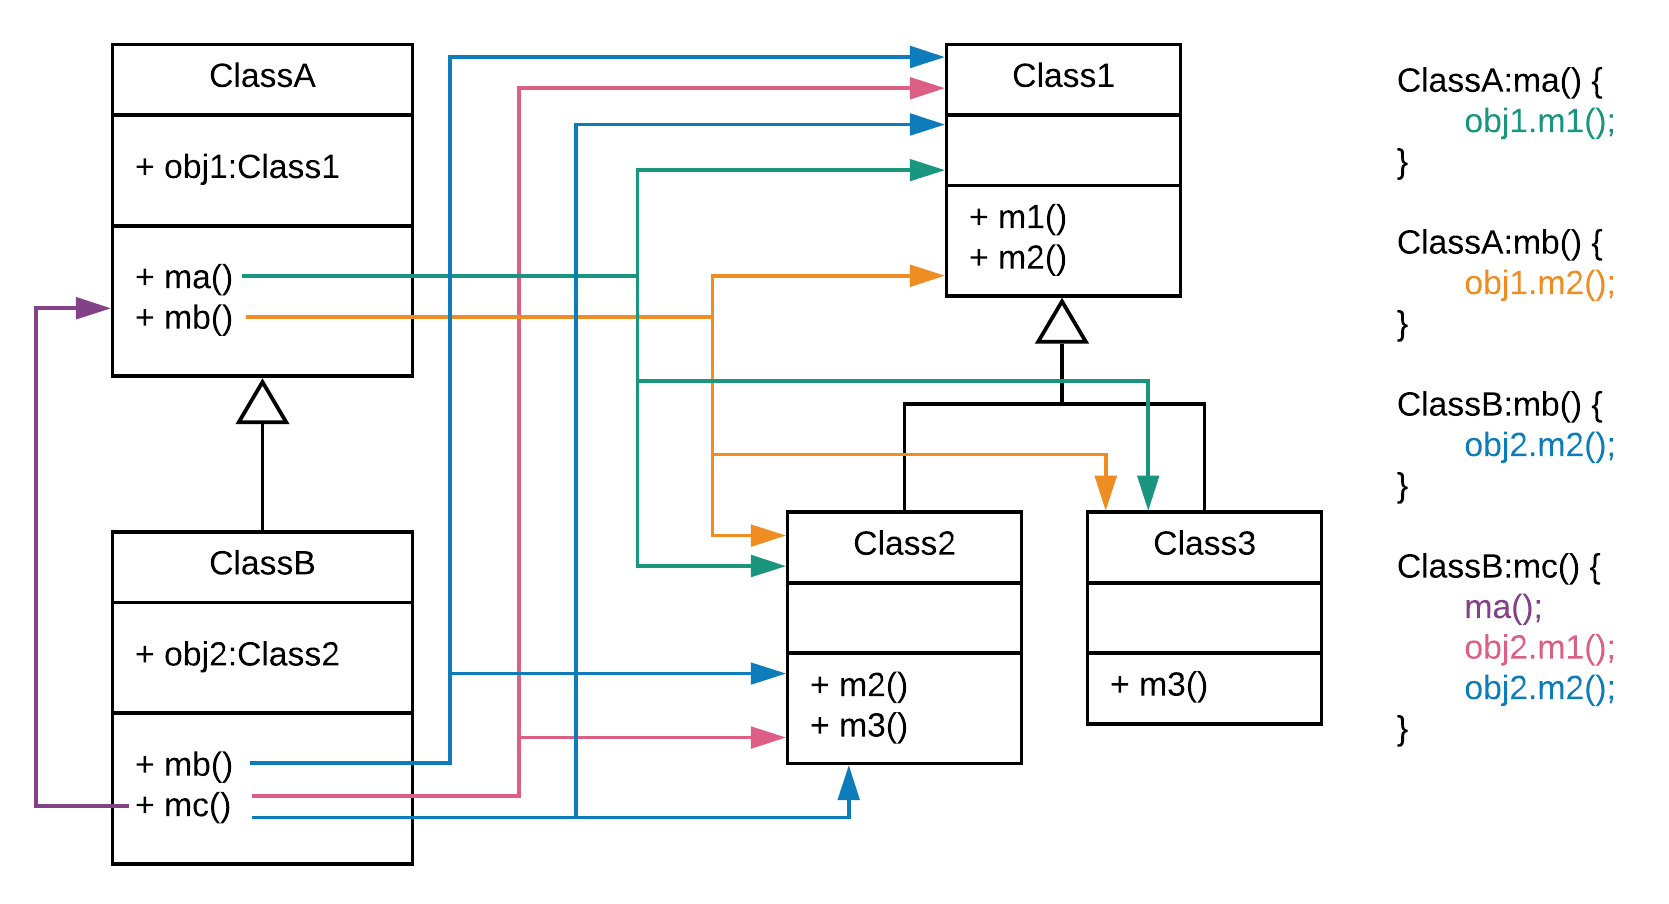
\includegraphics[width=\textwidth]{figures/specialcases.png}
\caption{Example of coupling special cases, based on example from Briand et al. \cite{briand1999unified}}
\label{fig:specialcases}
\end{center}
\end{figure}

In order to answer the first question, we focus on the method \texttt{mc} of \texttt{ClassB} in Figure \ref{fig:specialcases}. This method invokes \texttt{ma} of \texttt{ClassA}, inherited by \texttt{ClassB}.

This is known as \textit{inheritance-based} coupling and is sometimes considered as a special case of coupling.
When there is a change of an inherited method that a class uses, it requires the same maintenance as the method that is not inherited. Therefore, our metrics  \textbf{include inheritance-based coupling without distinction}.

In the case of the second question, polymorphism, we look at the methods of \texttt{ClassA}. This class contains an attribute of type \texttt{Class1}, which considering dynamic assignation of types could also be of type \texttt{Class2} or \texttt{Class3}.

We first analyze whether a call to a method of \texttt{Class1} would create coupling with \texttt{Class2} and \texttt{Class3}, and if it makes a difference when the method is overridden or not. The method \texttt{ma} invokes \texttt{m1}, which is not overridden by any of the descendants of \texttt{Class1}. When a change is made in \texttt{Class2} or \texttt{Class3} no change is required as the invoked method remains the same. In contrast, method \texttt{mb} calls \texttt{m2}, which is overridden in \texttt{Class2}. Here, the implementation of \texttt{m2} in \texttt{Class2} could be updated, and this may affect the way \texttt{ClassA} uses it, and therefore changes may be needed. Thus, it is necessary to \textbf{account for polymorphism}.

Lastly, we discuss about how to decide whether a method belongs to a class or not. We have two options: (1) a method belongs to the class that implements it (could be more than one since we account for polymorphism), or (2) a method belongs to the class that it is referenced from. An example of this can be found in the last two lines of the method \texttt{mc} of \texttt{ClassB} call method \texttt{m1} and \texttt{m2} on an object of type \texttt{Class2}. The difference is that \texttt{m1} is implemented in \texttt{Class1} and \texttt{m2} is overridden in \texttt{Class2}. From a maintenance perspective, when the method \texttt{m1} is updated in \texttt{Class1}, this probably requires update in \texttt{ClassB} as well. However, changes in \texttt{Class2} will not generate a need to update the method call in \texttt{ClassB}. When  \texttt{m2} is updated in \texttt{Class1}, it will not make a difference for this call to \texttt{m2} since it is not executing the implementation of \texttt{Class1}. Therefore, \textbf{a method call creates coupling with the class that contains the implementation}.

\paragraph{Result}
All the metrics that are used to measure the dependencies between libraries by considering coupling, are classified in Table \ref{table:metric-characteristics} according to the previous discussion on the criteria.

\begin{table}[h]
    \begin{center}
    \begin{tabular}{|l|l|l|l|l|l|l|l|l|}
    \hline
    \rot{Metric} & \rot{Type of connection} & \rot{Locus of impact} & \rot{Domain of measure} & \rot{Counting connections   } & \rot{Direct/Indirect} & \rot{Inheritance} & \rot{Polymorphism} & \rot{Item belongs to class} \\ \hline
    \hline
    \#1   & 6 & Import & Library & G & Direct   & Both, no distinction & Yes & Implemented \\\hline
    \#2   & 1 & Import & Library & G & Direct   & Both, no distinction & Yes & Implemented \\\hline
    \hline
    \#3   & 6 & Import & Library & G & Indirect & Both, no distinction & Yes & Implemented \\\hline
    \#4   & 1 & Import & Library & G & Indirect & Both, no distinction & Yes & Implemented \\\hline
    \end{tabular}
    \end{center}
    \caption{Criteria of the set of metrics}
    \label{table:metric-characteristics}
\end{table}

\subsection{Metrics for direct dependencies}\label{section:defMetrics}
This section begins with a brief discussion in which the definition of coupling of the proposed metrics is compared with the existing metrics in the literature described in Section \ref{section:bg-coupling}. Next, there is the formal definition of each of the metrics. To end the section, the metrics' theoretical validation is done by proving the five properties of coupling metrics for each one of the metrics.

\subsubsection{Revisiting existing metrics}
Once we have defined the coupling that is going to be measured by each of the metrics (see Table \ref{table:metric-characteristics}), we can compare it with the existing coupling metrics, according to Table \ref{table:coupling-metrics} in Section \ref{section:bg-coupling}.

\paragraph{Metric \#1}
To compare the coupling defined for this first metric defined in Table \ref{table:metric-characteristics} with the existing metrics, we focus on the ones that have the following characteristics:

\begin{itemize}
  \item Type of connection: method invocations (type 6 in Table \ref{table:types-connections})
  \item Locus of impact: import
  \item Direct or indirect coupling: direct
  \item Counting connections: count individual connections (option A or C in Table \ref{table:counting-connections}).
\end{itemize}

The metrics that share these characteristics are \textit{MPC}, the group \textit{ICP}, and the metrics \textit{AMMIC}, \textit{IFMMIC} and \textit{OMMIC}. However, \textit{MPC} does not consider polymorphic implementations of the called methods. \textit{IFMMIC} is a metric formulated specifically for C++ \cite{briand1997investigation} and therefore is not useful for our model.

From the group of metrics \textit{ICP}, the metric \textit{ICP}  considers both inheritance and non-inheritance coupling and therefore shares the definition of coupling with our metric. Nevertheless, according to the definition of \textit{ICP}, the coupling created by each method call is weighted by the number of parameters of the called method. In this aspect, it differs from metric \#1 from Table \ref{table:metric-characteristics}.

Finally, the metrics \textit{AMMIC} and \textit{OMMIC} use the same definition of coupling as metric \#1 except that \textit{AMMIC} counts the method invocations to ancestors and \textit{OMMIC} to other classes. Therefore, metric \#1 is the sum of \textit{AMMIC} and \textit{OMMIC} but aggregated to the library aggregation level instead of class level.

\paragraph{Metric \#2}
In the case of the second metric as defined in Table \ref{table:metric-characteristics}, we focus on the metrics with the following characteristics:

\begin{itemize}
  \item Type of connection: client class contains an attribute of type server class, aggregation coupling (type 1 in Table \ref{table:types-connections})
  \item Locus of impact: import
  \item Direct or indirect coupling: direct
  \item Counting connections: count individual connections (option A or C in Table \ref{table:counting-connections})
\end{itemize}

According to Table \ref{table:coupling-metrics}, the metrics that share these characteristics are \textit{DAC}, and from the suite of metrics by Briand et al. \cite{briand1997investigation} the metrics \textit{IFCAIC}, \textit{ACAIC} and \textit{OCAIC}. However, \textit{IFCAIC} is an extension for C++ and will not be considered.

According to the definition of \textit{DAC}, it counts the number of attributes of a class that have any other class as type. Therefore, instead of calculating the coupling between two classes, it calculates a class's coupling with every other class. However, metric \#2 is used at the library level and calculates coupling between two libraries instead of the coupling of one library with all the others.

Finally, \textit{ACAIC} and \textit{OCAIC} consider aggregation coupling with ancestors and others respectively. Therefore, metric  \#2 is the sum of these two metrics, but aggregated to library aggregation level, since the metrics are designed for class level.

\subsubsection{Formal definition}\label{subsec:metric-definition}

\paragraph{Metric \#1: Direct method invocation coupling (\texttt{MIC})}
The $\verb|MIC|$ metric measures the dependency between two libraries, one acting as a client ($L_c$) and the other as a server ($L_s$).
Based on the granularity of the measure criterion discussed in Section~\ref{subsect:defCoupling}, this metric is calculated for each of the classes implemented in $L_c$, and for each of the methods implemented $\verb|M|(L_c)$ in these classes. For each implemented method  $m_c \in \verb|M|(L_c)$, we count the number of individual invocations to a method of $L_s$, denoted $\verb|nII|(m_c,L_s)$. For each method invocation made by the methods implemented in $L_c$, we count only the ones implemented in stable classes (not implemented in $L_c$). The set of stable methods invoked is denoted $\verb|SIM|(m_c)$.

\begin{equation}
\label{eqn:mic}
\verb|MIC|(L_c, L_s) =\!\!\!\!\! \sum_{m_c \in \verb|M|(L_c)} \verb|nII|(m_c, L_s)
\end{equation}

According to the criterion inheritance, it is necessary to consider all the polymorphic implementations of the invoked method that are implemented in $L_s$. Therefore, we intersect the set of polymorphic implementations of an invoked method $\verb|PM|(m_s)$ with the set of methods $\verb|M|(L_s)$ implemented in $L_s$. Finally, to obtain the number of individual invocations, $\verb|nII|(m_c,L_s)$, we multiply the number of times a stable method ($m_s \in \verb|SIM|(m_c)$) has been invoked, $\verb|nI|(m_c, m_s)$ by the number of polymorphic implementations $\verb|nP|(m_s, L_s)$ of the method in $L_s$.

\begin{equation}
\label{eqn:mic-nii}
   \verb|nII|(m_c, L_s) = \sum_{m_s \in \verb|SIM|(m_c)} \verb|nI|(m_c, m_s)*\verb|nP|(m_s, L_s)
\end{equation}

\begin{equation}
\label{eqn:mic-np}
    \verb|nP|(m_s, L_s) = |\verb|PM|(m_s) \cap \verb|M|(L_s)|
\end{equation}

\paragraph{Metric \#2: Direct aggregation coupling (\texttt{AC})}

The $\verb|AC|$ metric counts the number of times when a class of $L_c$ has an attribute whose type is a class implemented in $L_s$. Therefore, the metric is calculated for each class implemented in $L_c$ ($\verb|C|(L_c)$). We consider only those attributes types that are stable classes (not implemented in $L_c$) for each class. The set of stable attribute types in a class $c$ is $\verb|SAT|(c_c)$.

To account for polymorphism (criterion \textit{inheritance}), we count all the descendants of the class that are implemented in $L_s$. Therefore, we intersect the set of the descendants of the class, $\verb|DC|(c_s)$, with the set of
classes implemented in $L_s$ ($\verb|C|(L_s)$). Finally, to count the  individual connections, we multiply the number of times a client class $c_c$ has an attribute of type the server class $c_s$ $\verb|NA|(c_c, c_s)$ by the number of class descendants (class included) implemented in $L_s$ ($\verb|nDC|(c_s,L_s)$).

\begin{equation}
\label{eqn:ac}
  \verb|AC|(L_c,L_s) = \!\!\!\!\sum_{c_c \in \verb|C|(L_c)} \sum_{c_s \in \verb|SAT|(c_c)} \!\!\!\!\verb|NA|(c_c, c_s)*\verb|nDC|(c_s, L_s)
\end{equation}

\begin{equation}
\label{eqn:ac-ndc}
    \verb|nDC|(c_s, L_s) = |\verb|DC|(c_s) \cap \verb|C|(L_s)|
\end{equation}

\subsubsection{Theoretical validation}
\unsure{Should I move the description of the properties to background, or is it fine here?}
The theoretical validation of the metrics consists of demonstrating the properties of the metrics. Theoretical validation is necessary since it proves that the metrics share some properties with the attribute; these metrics measure coupling. In particular, for coupling metrics, there are five properties defined by Briand et al. \cite{briand1996property}, which have been largely used by the literature \cite{poshyvanyk2006conceptual, allen1999measuring, zhao2004measuring}.

For the description of the properties, we use $\verb|Coupling|(L_c, L_s)$ to refer to both $\verb|AC|$ and $\verb|MIC|$, and $\verb|R|(L_c, L_s)$ to refer to the set of relationships between $L_c$ and $L_s$. $\verb|Coupling|(L_c, L_s)$ uses $\verb|R|(L_c, L_s)$ to evaluate the coupling between the two elements, but the way it is used differs per metric. The description of the properties is based on the description done by Briand et al. \cite{briand1996property}, which was meant for coupling metrics that measure the coupling within an element, or between an element and all the other elements. Therefore, the properties' description has been adapted for metrics that measure coupling between two different elements. Also, since all the defined metrics measure import coupling, the properties' definitions are focused on this locus of impact.

\paragraph{Property 1: Nonnegativity}

Let $L_c$ be a client library and $L_s$ be a server library. The coupling between the two libraries is non-negative. $\verb|Coupling|(L_c, L_s) \ge 0$.

\paragraph{Property 2: Null value}
Coupling is expected to be null (zero) when there is no import relationship between the client and the server libraries.

Let $L_c$ be a client library and $L_s$ be a server library. The coupling between the two libraries is null if the set of import relationships from $L_c$ to $L_s$, $\verb|R|(L_c, L_s)$, is empty. Therefore, $\verb|R|(L_c, L_s) = \emptyset \implies \verb|Coupling|(L_c, L_s) = 0$.

\paragraph{Property 3: Monotonicity}
Considering the definition of coupling, it is expected that when more relationships are added between the libraries, coupling does not decrease.

Let $L_c$ be a client library, $L_s$ be a server library, and $c \in L_c$ be a class in $L_c$. If we modify class $c$ to form a new class $c'$ which is identical to $c$ except that $\verb|R|(c, L_s) \subseteq \verb|R|(c', L_s)$. For example, some method invocations have been added from $c$ to classes implemented in $L_s$. Let $L_c'$ be a library identical to $L_c$ but in which $c$ has been replaced by $c'$. Then, $\verb|Coupling|(L_c, L_s) \le \verb|Coupling|(L_c', L_s)$.

\paragraph{Property 4: Merging of classes}
The original definition of the property is created for metrics that measure coupling within a system, and therefore it is necessary to reformulate it. It is expected that if two classes of a system are merged, the system's coupling does not increase. If two classes are merged, the coupling between the two classes is subtracted from the system's total coupling.

When considering the coupling between a client library and a server library, if two client library classes are merged, the two libraries' coupling would not increase. It could decrease, depending on how the refactoring is performed. If the classes share usage of the server library, one of the usages may be removed.

Therefore, let $L_c$ be a client library, $L_s$ be a server library, and $c_1, c_2 \in L_c$ two classes in $L_c$. Let $c'$ be the class that results from merging  $c_1$ and $c_2$, and $L_c'$ be the library resulting from $L_c$ when $c_1$ and $c_2$ have been replaced by $c'$. Then, $\verb|Coupling|(c_1, L_s) + \verb|Coupling|(c_2, L_s) \ge \verb|Coupling|(c', L_s)$ and $\verb|Coupling|(C, L_s) \ge \verb|Coupling|(C', L_s)$.

\paragraph{Property 5: Merging of unconnected classes}
This property is a variation of the previous one, and it has to be adapted to the use case of this thesis. It is expected that the system's coupling will stay the same if two classes of a system, which have no relationship, are merged. This is because the class that results in the merging will have the same number of relationships with other classes as the original two.

When measuring the coupling between a client library and a server library, the two unconnected classes are not using the server library in the same way. Therefore, none of the relationships with the server library can be merged when merging the two classes, and the coupling with the server library stays the same.

Let $L_c$ be a client library, $L_s$ a server library, and $c_1, c_2 \in L_c$ two classes from $L_c$ which do not share the same relationship with $L_s$. Let $c'$ be the class that is the union of  $c_1$ and $c_2$, and $L_c'$ be the library identical to $L_c$ but in which $c_1$ and $c_2$ have been replaced by $c'$. If there are no relationships between $c_1$ and $c_2$, then, $\verb|Coupling|(c_1, L_s) + \verb|Coupling|(c_2, L_s) = \verb|Coupling|(c', L_s)$ and $\verb|Coupling|(L_c, L_s) = \verb|Coupling|(L_c', L_s)$.

\subsubsection{Theoretical validation: MIC}

\paragraph{Property 1: Nonnegativity}
If we assume that the metric $\verb|MIC|$ does not fulfill the property Nonnegativity, there should be a client library $L_s$ and a server library $L_c$ such that $\verb|MIC|(L_c, L_s) < 0$.
According to the equation \ref{eqn:mic}, this means that exists at least one client method $m_c \in \verb|M|(L_c)$ such that $\verb|nII|(m_c, L_c) < 0$. Following the equation of $\verb|nII|$ \ref{eqn:mic-nii}, this opens two possibilities.

First, that there is a server method $m_s \in \verb|SIM|(m_c)$ such that $\verb|nI|(m_c, m_s) < 0$. However, $m_s$ is a method out of the set $\verb|SIM|(m_c)$ which is the set of stable methods invoked by $m_c$, which means that $\verb|nI|(m_c, m_s) > 0$ for all $m_s \in \verb|SIM|(m_c)$, therefore it is a contradiction.

The other option is that there is a method $m_s \in \verb|SIM|(m_c)$ such that $\verb|nP|(m_s, L_s) < 0$. $\verb|nP|(m_s, L_s)$, according to the equation \ref{eqn:mic-np}, corresponds to the cardinality of the intersection between the set $\verb|PM|(m_s)$ and $\verb|M|(L_s)$. Therefore, the cardinality of the intersection has to be less than zero. However, the cardinality of the intersection is by definition greater or equal to zero. This constitutes a contradiction.

Therefore, the initial assumption is not true, and \textit{Nonnegativity} holds for the metric $\verb|MIC|$.

\paragraph{Property 2: Null value}
Assuming there is no null value for metric $\verb|MIC|$, there is a client library $L_c$ and a server library $L_s$ such that $\verb|R|(L_c, L_s) = \emptyset$, and $\verb|MIC|(L_c, L_s)	\neq 0$. As non-negativity holds, we have that $\verb|MIC|(L_c, L_s) \ge 0$. Therefore, $\verb|MIC|(L_c, L_s) > 0$. Hence, following equation \ref{eqn:mic} there is a client method $m_c \in M(L_c)$ such that $\verb|nII|(m_c, L_s) > 0$.

Thus, according to equation \ref{eqn:mic-nii}, there is a server method $m_s \in \verb|SIM|(m_c)$, such that $\verb|nI|(m_c, m_s) > 0$ and $\verb|nP|(m_s, L_s) > 0$. Therefore, the method $m_s$ is called at least one time by the method $m_c$ from the client library $L_c$, and at the same time is implemented by the server library $L_s$, which means that there is a relationship between $L_c$ and $L_s$, which contradicts the original assumption that $\verb|R|(L_c, L_s) = 0$.

Consequently, there is a \textit{null value} for metric $\verb|MIC|$.

\paragraph{Property 3: Monotonicity}
Let $L_c$ be a client library that contains class $c_c$, and let $c_c'$ be a class resulting from adding relationships with the server library $L_s$ to the class $c_c$. Then, $\verb|R|(c_c, L_s) \subseteq \verb|R|(c_c', L_s)$. Let $L_c'$ be a client library identical to $L_c$ but in which the class $c_c$ has been replaced by $c_c'$. Therefore, $\verb|R|(L_c, L_s) \subseteq \verb|R|(L_c', L_s)$.

Let's assume that the $\verb|MIC|$ metric does not fulfill the property monotonicity, this would mean that $\verb|MIC|(L_c, L_s) > \verb|MIC|(L_c', L_s)$. Since the only difference between $L_c$ and $L_c'$ is the substitution of $c_c$ by $c_c'$, then $\sum_{m_c \in \verb|M|(c_c)} \verb|nII|(m_c, L_s) > \sum_{m_c' \in \verb|M|(c_c')} \verb|nII|(m_c', L_s)$ (see equation \ref{eqn:mic}). Therefore, the methods of class $c_c$ have more individual invocations to $L_s$ than the methods from class $c_c'$. This contradicts the initial assumption that $\verb|R|(c_c, L_s) \subseteq \verb|R|(c_c', L_s)$.

Therefore, \textit{Monotonicity} holds for the metric $\verb|MIC|$.

\paragraph{Property 4: Merging of classes}
Let $L_c$ be a client library that includes the classes $c_1$ and $c_2$. Let $c'$ be a class such that $c_1 + c_2 = c'$ and $L_c'$ be a client library identical to $L_c$ but where $c_1$ and $c_2$ have been replaced by $c'$. If we assume that the property merging of classes does not hold for metric $\verb|MIC|$, it would mean that $\verb|R|(c_1, L_s) \subseteq \verb|R|(c', L_s) \land \verb|R|(c_2, L_s) \subseteq \verb|R|(c', L_s)$ and at the same time $\verb|MIC|(L_c, L_s) > \verb|MIC|(L_c', L_s)$.

Therefore, there is a method $m_c$ which is implemented in $c_1$ or $c_2$ such that contains a call to a method $m_s$ which does not exist in any of the methods implemented in $c'$. This is a contradition with the initial affirmation $\verb|R|(c_1, L_s) \subseteq \verb|R|(c', L_s) \land \verb|R|(c_2, L_s) \subseteq \verb|R|(c', L_s)$. Therefore, the property \textit{Merging of classes} holds for metric $\verb|MIC|$.

\paragraph{Property 5: Merging of unconnected classes}
Let $L_c$ be a client library and $L_s$ be a server library. Let $c_1$ and $c_2$ be classes implemented in $L_c$, such that $\verb|R|(c_1, L_s) \cap \verb|R|(c_2, L_s) = \emptyset$. Let $c'$ be a class such that $c_1 + c_2 = c'$. Therefore, $\verb|R|(c_1, L_s) + \verb|R|(c_2, L_s) = \verb|R|(c', L_s)$. Let $L_c'$ be a client library identical to $L_c$ but in which $c_1$ and $c_2$ have been replaced by $c'$. We assume that the metric $\verb|MIC|$ does not fulfill this property.

Therefore, $\verb|MIC|(L_c, L_s) \neq \verb|MIC|(L_c', L_s)$. According to property \textit{Merging of classes}, $\verb|MIC|(L_c, L_s)$ cannot be less than $\verb|MIC|(L_c', L_s)$. Thus, $\verb|MIC|(L_c, L_s) > \verb|MIC|(L_c', L_s)$. This means that there is a $m_c$ implemented in $c_1$ or $c_2$ that contains an invocation to a method $m_s$ implemented in $L_s$, which is not included in $c'$. This contradicts that $\verb|R|(c_1, L_s) + \verb|R|(c_2, L_s) = \verb|R|(c', L_s)$.

Therefore, property \textit{Merging of unconnected classes} holds for metric $\verb|MIC|$.

\subsubsection{Theoretical validation: AC}

\paragraph{Property 1: Nonnegativity}
Supose that the metric $\verb|AC|$ does not have the nonnegativity property. Thus, there is a client library $L_c$ and a server library $L_s$ such that $\verb|AC|(L_c, L_s) < 0$. Then, according to equation \ref{eqn:ac} there is a client class $c_c \in \verb|C|(L_c)$ and a server class $c_s \in \verb|SAT|(c_c)$ such that either $\verb|NA|(c_c, c_s)$ or $\verb|nDC|(c_s, L_s)$ have a negative value.

Let's assume that $\verb|NA|(c_c, c_s) < 0$. This means that the $c_s$ is a class that is included in the set of stable classes declared as fields in $c_c$ ($c_s \in \verb|SAT|(c_c)$) and, at the same time is declared a negative number of times, which is a contradiction.

Therefore, $\verb|nDC|(c_s, L_s)$ has to be negative. According to equation \ref{eqn:ac-ndc}, $\verb|nDC|(c_s, L_s)$ corresponds to the cardinality of the intersection between two sets. Even if the two sets do not share any element, by definition, the intersection will be the empty set, and the cardinality will be zero. Hence, $\verb|nDC|(c_s, L_s)$ cannot have a negative value, and the initial assumption is false.

In conclusion, \textit{Nonnegativity} holds for the metric $\verb|AC|$.

\paragraph{Property 2: Null value}
If we assume that property null value does not hold for metric $\verb|AC|$, there has to be a client library $L_c$ and a server library $L_s$ such that have no relationship ($\verb|R|(L_c, L_s) = 0$) and $\verb|AC|(L_c, L_s)	\neq 0$. Since $\verb|AC|$ has the property \textit{Nonnegativity}, the result cannot be negative, which means that $\verb|AC|(L_c, L_s) > 0$. Hence, following equation \ref{eqn:ac}, there is a client class $c_c \in \verb|C|(L_c)$ and a server class $c_s \in \verb|SAT|(c_c)$ such that $\verb|NA|(c_c, c_s) > 0$ and $\verb|nDC|(c_s, L_s) > 0$. This means that the class $c_s$ is at the same time declared at least once by the client class $c_c$ ($\verb|NA|(c_c, c_s) > 0$) and implemented in the server library $L_s$. However, this would create a relationship between $L_c$ and $L_s$, which contradicts the initial assumption.

 Therefore, the property \textit{Null value} holds for metric $\verb|AC|$.

\paragraph{Property 3: Monotonicity}
Let $L_c$ be a client library that contains class $c_c$, and let $c_c'$ be a class identical to $c_c$ but more relationships with the server library $L_s$. Then, $\verb|R|(c_c, L_s) \subseteq \verb|R|(c_c', L_s)$. Let $L_c'$ be a client library identical to $L_c$ but in which the class $c_c$ has been replaced by $c_c'$. Therefore, $\verb|R|(L_c, L_s) \subseteq \verb|R|(L_c', L_s)$.

If we assume that the metric $\verb|AC|$ does not fulfill this property, means that $\verb|AC|(L_c, L_s) > \verb|AC|(L_c', L_s)$. The only difference between these two calculations is the result of the calculation for $c_c$ and $c_c'$. Therefore, $\sum_{c_s \in \verb|SAT|(c_c)} \verb|NA|(c_c, c_s) * \verb|nDC|(c_s, L_s) > \sum_{c_s \in \verb|SAT|(c_c')} \verb|NA|(c_c', c_s) * \verb|nDC|(c_s, L_s)$, see equation \ref{eqn:ac}.

This means that there is a server class $c_s \in \verb|SAT|(c_c)$, that is implemented in $L_s$ ($\verb|nDC|(c_s, L_s) > 0$) such that $\verb|NA|(c_c, c_s) > \verb|NA|(c_c', c_s)$. This contradicts the original assumption that $c_c'$ is constructed from $c_c$ but with additional relationships with $L_s$. $\verb|NA|(c_c, c_s)$ will only be greater than $\verb|NA|(c_c', c_s)$ if there is an attribute of type $c_s$ in $c_c$ (which is a relationship between $c_c$ and $L_s$) that does not exist in $c_c'$.

Therefore, \textit{Monotonicity} holds for the metric $\verb|AC|$.

\paragraph{Property 4: Merging of classes}
Let $L_c$ be a client library that includes the classes $c_1$ and $c_2$. Let $c'$ be a class such that $c_1 + c_2 = c'$ and $L_c'$ be a client library identical to $L_c$ but where $c_1$ and $c_2$ have been replaced by $c'$. We assume that the property merging of classes does not hold for metric $\verb|AC|$. Therefore, $\verb|R|(c_1, L_s) \subseteq \verb|R|(c', L_s) \land \verb|R|(c_2, L_s) \subseteq \verb|R|(c', L_s)$ and, also $\verb|AC|(L_c, L_s) > \verb|AC|(L_c', L_s)$.

Thus, either $c_1$ or $c_2$ contain an attribute of type $c_s$, such that $c_s$ is implemented in $L_s$ and it is not included $c'$. This creates a contradition with the initial affirmation $\verb|R|(c_1, L_s) \subseteq \verb|R|(c', L_s) \land \verb|R|(c_2, L_s) \subseteq \verb|R|(c', L_s)$, since the declaration of an attribute of type $c_s$ is included in $\verb|R|(c_1, L_s)$ or $\verb|R|(c_2, L_s)$. Therefore, \textit{Merging of classes} holds for metric $\verb|AC|$.

\paragraph{Property 5: Merging of unconnected classes}
Let $L_c$ be a client library and $L_s$ be a server library. Let $c_1$ and $c_2$ be classes implemented in $L_c$, such that $\verb|R|(c_1, L_s) \cap \verb|R|(c_2, L_s) = \emptyset$. Let $c'$ be a class such that $c_1 + c_2 = c'$. Therefore, $\verb|R|(c_1, L_s) + \verb|R|(c_2, L_s) = \verb|R|(c', L_s)$. Let $L_c'$ be a client library identical to $L_c$ but in which $c_1$ and $c_2$ have been replaced by $c'$. We assume that the metric $\verb|AC|$ does not fulfill property \textit{Merging of unconnected classes}.

Therefore, $\verb|AC|(L_c, L_s) \neq \verb|AC|(L_c', L_s)$. According to property \textit{Merging of classes}, it cannot happen that $\verb|AC|(L_c, L_s) < \verb|AC|(L_c', L_s)$. Therefore, $\verb|AC|(L_c, L_s) > \verb|AC|(L_c', L_s)$. The only way this is if there is an attribute of type $c_s$ declared in $c_1$ or $c_2$ and implemented in $L_s$, such that is not included in $c'$. This creates a contradition with the initial affirmation that $\verb|R|(c_1, L_s) + \verb|R|(c_2, L_s) = \verb|R|(c', L_s)$.

Therefore, metric $\verb|AC|$ fulfills \textit{Merging of unconnected classes}.

\subsection{Metrics for transitive dependencies}\label{subsect:defMetricsTransitive}
In this section, the metrics to measure transitive dependencies are described. First, the characteristics of the metrics, according to the criteria previously discussed and summarized in Table \ref{table:metric-characteristics}, are compared to the existing metrics described in section \ref{section:bg-coupling}. Next, some concepts involved in the formulation of the transitive metrics are explained. Then, there is a formal definition of the two metrics for transitive dependencies. Finally, the five properties of coupling metrics are demonstrated.

\subsubsection{Revisiting existing metrics}
In the set of metrics reviewed by Briand et al. \cite{briand1999unified}, there is only one metric that does count indirect coupling, $RFC'$ (see Table \ref{table:coupling-metrics}). This metric also counts inheritance-based coupling, and it is focused on the client element, just as the metrics \#3 and \#4 defined in Table \ref{table:metric-characteristics}. However, $RFC'$ is calculated at the class aggregation level, whereas the metrics for this work are calculated at the library level. Furthermore, the strategy to count connections is E, which means that it counts the number of elements with which the class has a connection, not how many connections.

Therefore, both metrics \#3 and \#4 are different from those reviewed by Briand et al. \cite{briand1999unified}.

\subsubsection{Concepts related to transitive dependencies}\improvement{should this go in background instead?}
Other factors have to be taken into account to define the coupling for transitive metrics, which are not needed for the direct metrics.

\paragraph{Reachability}
To measure the transitive dependencies, only those methods or classes of the transitive dependencies that are \textit{reachable} from the analysed client library. For a given call-graph, a method is reachable if there is a path from the client library to the method. For example, in Figure \ref{fig:reachability}, there is no path from \texttt{Lib1} (the client library) to the method \texttt{Method10}. Therefore, \texttt{Method10} is not reachable form \texttt{Lib1} and the call from \texttt{Method6} to \texttt{Method10} will not be considered when measuring the transitive dependency between \texttt{Lib1} and \texttt{Lib3}, in the case of method invocation coupling.

\begin{figure}[ht]
\begin{center}
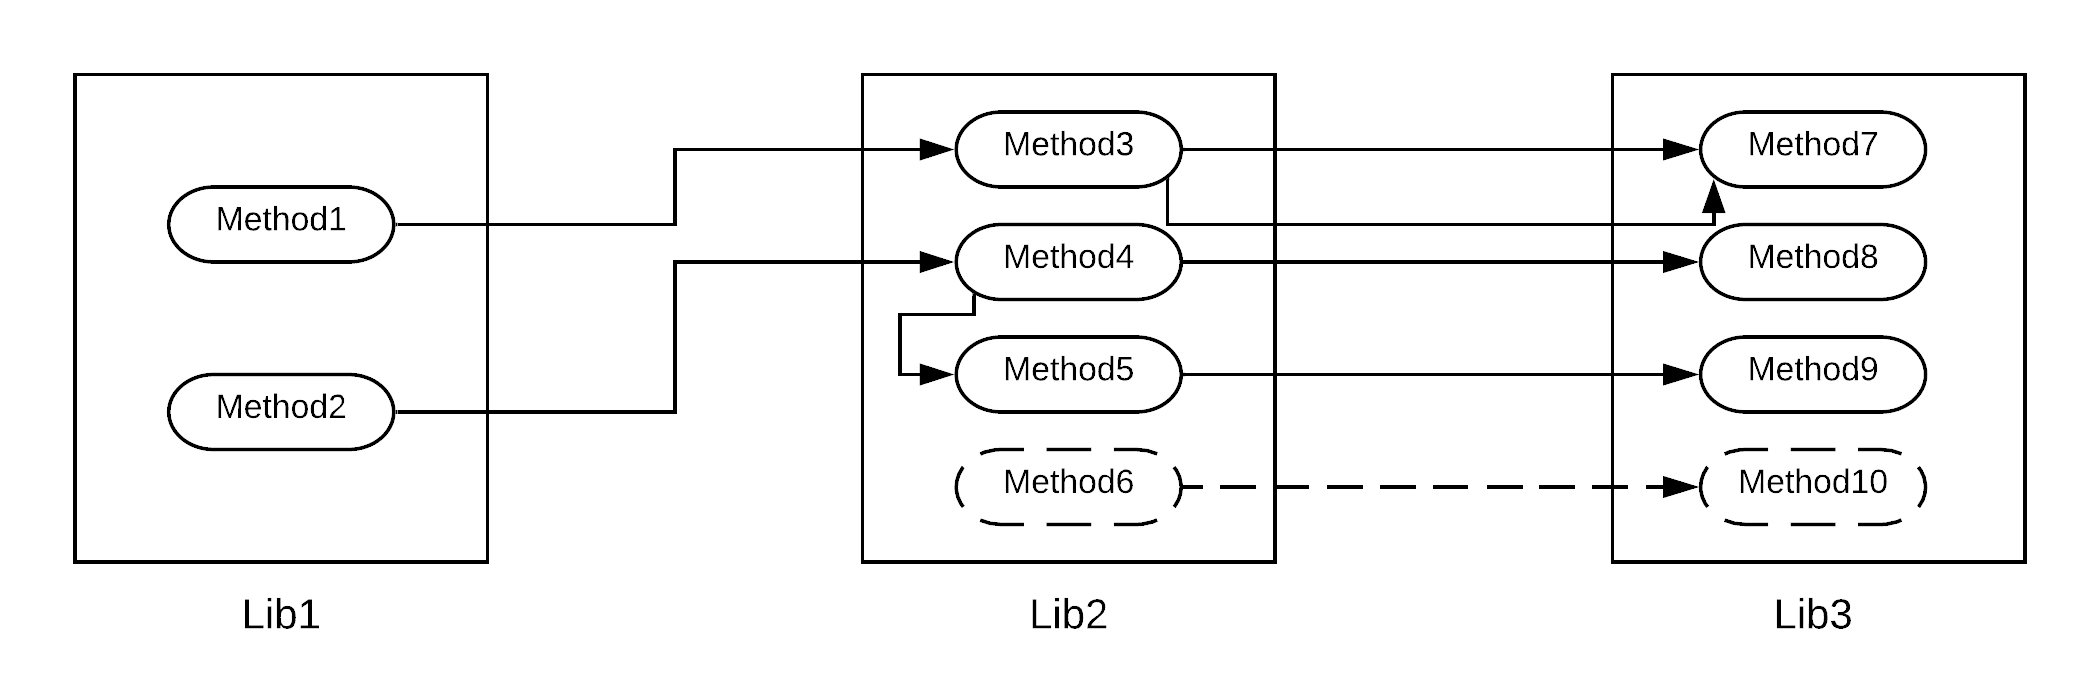
\includegraphics[width=\textwidth]{figures/Reachability.png}
\caption{Reachability example}
\label{fig:reachability}
\end{center}
\end{figure}

\paragraph{Propagation Factor}
The propagation represents how the impact of a change can spread across dependencies. In Figure \ref{fig:reachability}, a change in \texttt{Method3} would affect directly the client  library (\texttt{Lib1}). However, a change in \texttt{Method7}, affects first \texttt{Method3}, and then it can spread to \texttt{Method1}, in case it is not mitigated in \texttt{Method3}. This possible mitigation is accounted for by the \textit{Propagation Factor}.

\subsubsection{Formal definition}

\paragraph{Metric \#3: Transitive method invocation coupling (\texttt{TMIC})}
\todo{decide what to call each formula and whether to use indirect or transitive or something else}
If we look at how the metric $\verb|MIC|$ is calculated, it could be summarized as follows: find all the methods in $L_s$ that are reachable from $L_c$. Then, for each one, count how many method calls exist in $L_c$ that reach this method, and sum up the results. The main difference between $\verb|MIC|$ and $\verb|TMIC|$ is that the calls in $L_c$ will not directly execute a reachable method of $L_s$. The execution of a method in $L_s$ is indirect since $L_s$ is not a direct dependency of $L_c$.

Therefore, it is necessary to take into account the distance between $L_c$ and $L_s$. In addition, it could happen that $L_s$ is reachable from $L_c$ at different distances. For instance, if $L_s$ appeared twice in the dependency tree of $L_c$, this is is the case in Figure \ref{fig:dependency-tree} if we take \texttt{Lib1} as $L_c$ and \textit{Lib4} as $L_s$.

\begin{figure}[ht]
\begin{center}
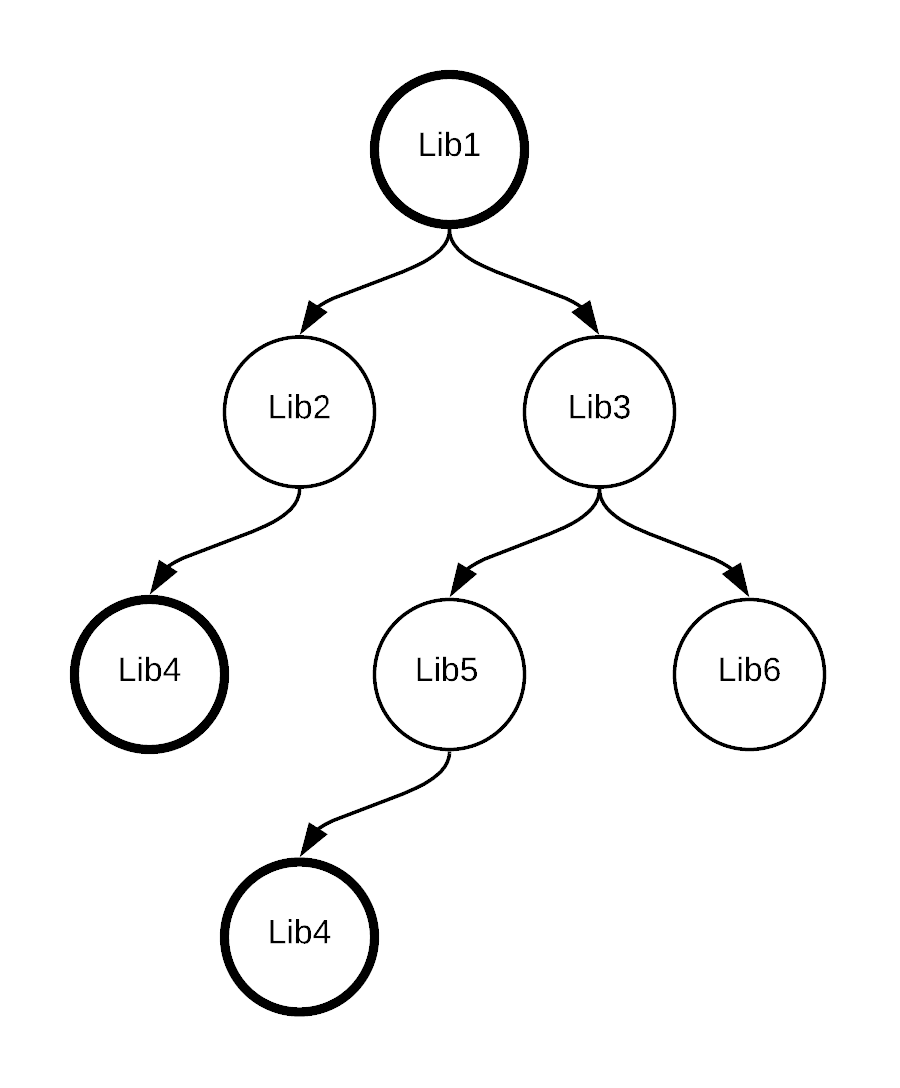
\includegraphics[width=0.4\textwidth]{figures/Thesis-DependencyTree.png}
\caption{Example dependency tree}
\label{fig:dependency-tree}
\end{center}
\end{figure}

Therefore, the coupling will be measured for a certain $\verb|distance|$, denoted $\verb|TMICD|(L_c,L_s, \verb|distance|)$.
The value of the metric $\verb|TMIC|(L_c,L_s)$, will be measured as follows. For each $\verb|distance|$ at which there is coupling between $L_c$ and $L_s$, sum up the coupling measured by $\verb|TMICD|(L_c,L_s, \verb|distance|)$, multiplied by a propagation factor ($\verb|PF|$) to the power of the $\verb|distance| - 1$. Where $\verb|PF| \in (0,1)$. We have designed the formula by taking the propagation factor to the power of $\verb|distance| - 1$, because this way, the coupling of the direct dependencies ($\verb|distance| = 1$) is not mitigated. Also, then when $\verb|distance| = 2$, which corresponds to the first level of transitivity, the coupling is mitigated only once.

\begin{equation}
\label{eqn:tmic}
  \verb|TMIC|(L_c,L_s) = \sum_{\verb|distance|} \verb|TMICD|(L_c,L_s, \verb|distance|) * \verb|PF|^{\verb|distance| - 1}
\end{equation}

The transitive coupling between two libraries at a certain distance $\verb|TMICD|(L_c, L_s, \verb|distance|)$ is calculated in the following manner. For each method from $L_s$ that is reachable from $L_c$ throught method calls at $\verb|distance|$ ($rm \in \verb|RM|(L_c,L_s,\verb|distance|)$), we count the number of method invocations in $L_c$ from which $rm$ is reachable, $\verb|nIR|(rm, L_c)$. The number of method invocations is multiplied by the number of polymorphic implementations of $rm$ in $L_s$ ($\verb|nDC|(rm, L_s)$).

\begin{equation}
\label{eqn:imic}
  \verb|TMICD|(L_c,L_s,\verb|distance|) = \sum_{rm \in \verb|RM|(L_c,L_s,\verb|distance|)} \verb|nIR|(rm,L_c) * \verb|nP|(rm, L_s)
\end{equation}

\paragraph{Metric \#4: Transitive aggregation coupling (\texttt{TAC})}
To calculate $\verb|TAC|$, just as in the case of $\verb|TMIC|$, the $\verb|distance|$ between $L_c$ and $L_s$ should be considered. Therefore, for each $\verb|distance|$, we take the number measured by $\verb|TACD|(L_c,L_s, \verb|distance|)$, and multiply it by a propagation factor $\verb|PF|$ to the power of the $\verb|distance| - 1$.

\begin{equation}
\label{eqn:tac}
  \verb|TAC|(L_c,L_s) = \sum_{\verb|distance|} \verb|TACD|(L_c,L_s, \verb|distance|) * \verb|PF|^{\verb|distance| - 1}
\end{equation}

The transitive aggregation coupling per distance ($\verb|TACD|(L_c, L_s, \verb|distance|)$), is calculated in the following way. For each class of $L_s$ that is reachable from $L_c$ through field declarations at $\verb|distance|$ ($rc \in \verb|RC|(L_c,L_s,\verb|distance|)$), count all the field declarations from which it is reachable ($\verb|nFR|(rc,L_c)$), and multiply it by the number of descendants of the reachable class ($\verb|nDC|(rm, L_s)$).

\begin{equation}
\label{eqn:iac}
  \verb|TACD|(L_c,L_s,\verb|distance|) = \sum_{rc \in \verb|RC|(L_c,L_s,\verb|distance|)} \verb|nFR|(rc,L_c) * \verb|nDC|(rm, L_s)
\end{equation}

\subsubsection{Theoretical validation: TMIC}

\paragraph{Property 1: Nonnegativity}
Assume that nonnegativity does not hold for metric $\verb|TMIC|$. Then, there exists a client library $L_c$, and a server library $L_s$ such that $\verb|TMIC|(L_c, L_s) < 0$. According to equation \ref{eqn:tmic}, there is a $\verb|distance|$ for which either $\verb|TMICD|(L_c,L_s, \verb|distance|) < 0$ or $\verb|PF|^{\verb|distance - 1|} < 0$. Since $\verb|distance|$ is a positive integer, and $\verb|PF| \in (0,1)$, the second option is not possible.

Let's assume that $\verb|TMICD|(L_c,L_s, \verb|distance|) < 0$. Looking at the equation \ref{eqn:imic}, we see that there has to be at least one method, $rm$, from $L_s$ and reachable from $L_c$ at a certain distance ($rm \in \verb|RM|(L_c,L_s,\verb|distance|)$), such that $\verb|nIR|(rm,L_c) < 0$ or $\verb|nP|(rm, L_s) < 0$. Since $\verb|nP|(rm, L_s)$ corresponds to the number of polymorphic implementations of $rm$ in $L_s$, and we know that $rm$ belongs to $L_s$, then $\verb|nP|(rm, L_s) \geq 1$. Finally, for $\verb|nIR|(rm,L_c) < 0$ to be true, there should be less than zero method invocations in $L_c$ from which $rm$ is reachable. However, since $rm \in \verb|RM|(L_c,L_s,\verb|distance|)$, and $\verb|RM|(L_c,L_s,\verb|distance|)$ corresponds to the set of methods from $L_s$ that are reachable from $L_c$, we have that $\verb|nIR|(rm,L_c) \geq 1$, which constitutes a contradition.

Therefore, the metric $\verb|TMIC|$ fulfills the property \textit{Nonnegativity}.

\paragraph{Property 2: Null value}
Assuming that $\verb|TMIC|$ does not fulfill property \textit{Null value}, there exists a client library $L_c$, and a server library $L_s$ such that $\verb|R|(L_c, L_s) = \emptyset$ and $\verb|TMIC|(L_c, L_s) \neq 0$.

For $\verb|TMIC|(L_c, L_s) \neq 0$ to be true, according to equation \ref{eqn:imic}, there has to be a method $rm$ such that  $rm \in \verb|RM|(L_c,L_s,\verb|distance|)$. However, that would mean that $rm$ belongs to $L_s$, and is reachable from $L_c$, which constitutes a relation between $L_c$ and $L_s$, and contradicts $\verb|R|(L_c, L_s) = \emptyset$.

Hence, the property \textit{null value} holds for metric $\verb|TMIC|$ .

\paragraph{Property 3: Monotonicity}
Let $L_c$ be a client library containing class $c_c$, and $c_c'$ be a class resulting from adding relationships with the server library $L_s$ to class $c_c$. Then, $\verb|R|(c_c, L_s) \subseteq \verb|R|(c_c', L_s)$. Let $L_c'$ be a client library resulting from replacing class $c_c$ by $c_c'$ in $L_c$. Therefore, $\verb|R|(L_c, L_s) \subseteq \verb|R|(L_c', L_s)$.

If we assume that $\verb|TMIC|$ does not fulfill property \textit{Monotonicity}, it would be true that $\verb|TMIC|(L_c, L_s) > \verb|TMIC|(L_c', L_s)$. Therefore, for a certain distance, we have that $\verb|TMICD|(L_c,L_s,\verb|distance|) > \verb|TMICD|(L_c',L_s,\verb|distance|)$, according to equation \ref{eqn:tmic}. According to the equation \ref{eqn:imic}, this opens two possibilities.

First, we have that $|\verb|RM|(L_c,L_s,\verb|distance|)| > |\verb|RM|(L_c',L_s,\verb|distance|)|$, which means that there are more methods from $L_s$ reachable from $L_c$ than from $L_c'$. This is not possible since, the only difference between $L_c$ and $L_c'$ is the substitution of class $c_c$ by class $c_c'$, which only adds relationships with $L_s$.

The second option is that for a certain $rm \in \verb|RM|(L_c,L_s,\verb|distance|)$, and therefore also $rm \in \verb|RM|(L_c',L_s,\verb|distance|)$, such that   $\verb|nIR|(rm,L_c) > \verb|nIR|(rm,L_c')$. However, that means that in $L_c$ there are more method invocations that reach $rm$, than in $L_c'$. As discussed earlier, this constitutes a contradicion with the way $L_c'$ is created.

Therefore, property 3 \textit{Monotonicity} holds for $\verb|TMIC|$.

\paragraph{Property 4: Merging of classes}
Let $L_c$ be a client library that includes the classes $c_1$ and $c_2$. Let $c'$ be a class such that $c_1 + c_2 = c'$ and $L_c'$ be a client library resulting from replacing $c_1$ and $c_2$ by $c'$ in $L_c$. If we assume that the property merging of classes does not hold for $\verb|TMIC|$, then $\verb|R|(c_1, L_s) \subseteq \verb|R|(c', L_s) \land \verb|R|(c_2, L_s) \subseteq \verb|R|(c', L_s)$ and $\verb|TMIC|(L_c, L_s) > \verb|TMIC|(L_c', L_s)$.

Since the only difference between $L_c$ and $L_c'$ is the replacement of $c_1$ and $c_2$ by $c'$, there has to be a method invocation from $c_1$ or $c_2$ to a method $rm \in \verb|RM|(L_c,L_s,\verb|distance|)$, which is not included in $c'$. However, the method invocation has to be a relation included in $\verb|R|(c_1, L_s)$ or $\verb|R|(c_2, L_s)$, and we have that $\verb|R|(c_1, L_s) \subseteq \verb|R|(c', L_s) \land \verb|R|(c_2, L_s) \subseteq \verb|R|(c', L_s)$. Therefore it is a contradiction.

Hence, the property \textit{Merging of classes} holds for $\verb|TMIC|$.

\paragraph{Property 5: Merging of unconnected classes}
Let $L_c$ be a client library and $L_s$ be a server library. Let $c_1$ and $c_2$ be classes implemented in $L_c$, such that $\verb|R|(c_1, L_s) \cap \verb|R|(c_2, L_s) = \emptyset$. Let $c'$ be a class such that $c_1 + c_2 = c'$. Therefore, $\verb|R|(c_1, L_s) + \verb|R|(c_2, L_s) = \verb|R|(c', L_s)$. Let $L_c'$ be a client library identical to $L_c$ but in which $c_1$ and $c_2$ have been replaced by $c'$. We assume that the metric $\verb|TMIC|$ does not fulfill this property.

Therefore, $\verb|TMIC|(L_c, L_s) \neq \verb|TMIC|(L_c', L_s)$. According to property \textit{Merging of classes}, $\verb|TMIC|(L_c, L_s) \geq \verb|TMIC|(L_c', L_s)$. Hence, $\verb|TMIC|(L_c, L_s) > \verb|TMIC|(L_c', L_s)$.

Then, there is a method invocation is $c_1$ or $c_2$ which is not included in $c$, which contradicts that $\verb|R|(c_1, L_s) + \verb|R|(c_2, L_s) = \verb|R|(c', L_s)$.

We conclude that $\verb|TMIC|$ fulfills property \textit{Merging of unconnected classes}.

\subsubsection{Theoretical validation: TAC}

\paragraph{Property 1: Nonnegativity}
Assuming that nonnegativity does not hold for metric $\verb|TAC|$, there exists a client library $L_c$, and a server library $L_s$ such that $\verb|TAC|(L_c, L_s) < 0$. In line with equation \ref{eqn:tac}, there is a $\verb|distance|$ for which two things can happen. First, $\verb|PF|^{\verb|distance| - 1} < 0$. However, since $\verb|distance|$ is a positive integer, and $\verb|PF| \in (0,1)$, this is not possible.

The second option is that $\verb|TACD|(L_c,L_s, \verb|distance|) < 0$. Looking at the equation \ref{eqn:iac}, we see that there has to be at least one class, $rc \in \verb|RC|(L_c,L_s,\verb|distance|)$, that belongs to $L_s$ and is reachable from $L_c$, such that $\verb|nFR|(rc,L_c) < 0$ or $\verb|nDC|(rm, L_s) < 0$. $\verb|nDC|(rm, L_s)$ is the number of descendants of $rc$ in $L_s$. As we know that $rc$ belongs to $L_s$, we have that $\verb|nDC|(rm, L_s) \geq 1$.

Finally, if $\verb|nFR|(rc,L_c) < 0$ is true, there are less than zero field declarations in $L_c$ from which $rc$ is reachable. However, since $rc \in \verb|RC|(L_c,L_s,\verb|distance|)$, and $\verb|RC|(L_c,L_s,\verb|distance|)$ corresponds to the set of classes from $L_s$ that are reachable from $L_c$ through field declarations, we have that $\verb|nFR|(rc,L_c) \geq 1$, which constitutes a contradition.

Therefore, the property \textit{Nonnegativity} holds for metric $\verb|TAC|$.

\paragraph{Property 2: Null value}
Let's assume that $\verb|TAC|$ does not fulfill property \textit{Null value}. Therefore, there exists a client library $L_c$, and a server library $L_s$ such that $\verb|R|(L_c, L_s) = \emptyset$ and $\verb|TAC|(L_c, L_s) \neq 0$.

If $\verb|TAC|(L_c, L_s) \neq 0$ then, as stated in equation \ref{eqn:iac}, there has to be a class $rc$ such that  $rc \in \verb|RC|(L_c,L_s,\verb|distance|)$. However, if $rc \in \verb|RC|(L_c,L_s,\verb|distance|)$, then $rc$ belongs to $L_s$, and is reachable from $L_c$. This creates a relation between $L_c$ and $L_s$, and therefore contradicts $\verb|R|(L_c, L_s) = \emptyset$.

In conclusion, the property \textit{Null value} holds for metric $\verb|TAC|$.

\paragraph{Property 3: Monotonicity}
Assuming that property \textit{Monotonicity} does not hold for metric $\verb|TAC|$, let $L_c$ be a client library containing class $c_c$, and $L_s$ be a server library. Also, let $c_c'$ be the resulting class of adding new relationships with $L_s$ to class $c_c$. Then, $\verb|R|(c_c, L_s) \subseteq \verb|R|(c_c', L_s)$. Let $L_c'$ be the client library resulting from replacing class $c_c$ by $c_c'$ in $L_c$. Therefore, $\verb|R|(L_c, L_s) \subseteq \verb|R|(L_c', L_s)$.

Since $\verb|TAC|$ does not fulfill property \textit{Monotonicity}, we have that $\verb|TAC|(L_c, L_s) > \verb|TAC|(L_c', L_s)$. Hence, for a certain distance, it is true that $\verb|TACD|(L_c,L_s,\verb|distance|) > \verb|TACD|(L_c',L_s,\verb|distance|)$, according to equation \ref{eqn:tac}. As equation \ref{eqn:iac} indicates, this can be true in two cases.

The first option is $|\verb|RC|(L_c,L_s,\verb|distance|)| > |\verb|RC|(L_c',L_s,\verb|distance|)|$.
In other words, there are more classes from $L_s$ reachable from $L_c$ than from $L_c'$. Since the only difference between $L_c$ and $L_c'$ is the replacement of class $c_c$ by $c_c'$, and according to the definition of class $c_c'$, this is not possible.

Therefore, the last option is that there is a class $rc \in \verb|RC|(L_c,L_s,\verb|distance|) \land rc \in \verb|RC|(L_c',L_s,\verb|distance|)$, such that   $\verb|nFR|(rc,L_c) > \verb|nFR|(rc,L_c')$. This implies that the number of field declarations that reach $rc$ in $L_c$is greater than in $L_c'$, which is a contradicion with the definition of $L_c'$.

Therefore, property \textit{Monotonicity} holds for $\verb|TAC|$.

\paragraph{Property 4: Merging of classes}
Let $L_c$ be a client library, and let classes $c_1$ and $c_2$ be classes implemented in $L_c$. Also, let $c'$, created as follows $c' = c_1 + c_2$, and $L_c'$ be a client library based on $L_c$ in which $c_1$ and $c_2$ have been replaced by $c'$. Assuming \textit{merging of classes} does not hold for $\verb|TAC|$, we have that $\verb|R|(c_1, L_s) \subseteq \verb|R|(c', L_s) \land \verb|R|(c_2, L_s) \subseteq \verb|R|(c', L_s) \land \verb|TAC|(L_c, L_s) > \verb|TAC|(L_c', L_s)$.

$L_c$ and $L_c'$ are only different in the replacement of $c_1$ and $c_2$ by $c'$. Hence, there has to be a field declaration from $c_1$ or $c_2$ which reaches a class $rc \in \verb|RC|(L_c,L_s,\verb|distance|)$, and is not found in $c'$. However, the reachability through a field declaration is a relation included in $\verb|R|(c_1, L_s)$ or $\verb|R|(c_2, L_s)$, and we have that $\verb|R|(c_1, L_s) \subseteq \verb|R|(c', L_s) \land \verb|R|(c_2, L_s) \subseteq \verb|R|(c', L_s)$, which constitutes a contradiction.

Therefore, $\verb|TAC|$ fulfills property \textit{Merging of classes}.

\paragraph{Property 5: Merging of unconnected classes}
Let $L_c$ and $L_s$ be a client and a server library respecively. Let $c_1$ and $c_2$ be classes implemented in $L_c$, such that $\verb|R|(c_1, L_s) \cap \verb|R|(c_2, L_s) = \emptyset$. Let $c'$ defined as $c' = c_1 + c_2$. Hence, $\verb|R|(c_1, L_s) + \verb|R|(c_2, L_s) = \verb|R|(c', L_s)$. Let $L_c'$ be a client library which is the result of replacing $c_1$ and $c_2$ by $c'$ in $L_c$.

Assume that the $\verb|TAC|$ does not fulfill \textit{Merging of unconnected classes}. This means that $\verb|TAC|(L_c, L_s) \neq \verb|TAC|(L_c', L_s)$. Since $\verb|TAC|$ has the property \textit{Merging of classes}, we know that $\verb|TAC|(L_c, L_s) \geq \verb|TAC|(L_c', L_s)$, which leaves $\verb|TAC|(L_c, L_s) > \verb|TAC|(L_c', L_s)$.

Then, there exists a field declaration in $c_1$ or $c_2$ which reaches a class included in $L_s$ and is not included in $c$. However, we have that $\verb|R|(c_1, L_s) + \verb|R|(c_2, L_s) = \verb|R|(c', L_s)$, which creates a contradiction.

Therefore, the metric $\verb|TAC|$ fulfills property \textit{Merging of unconnected classes}.

\section{Measuring usage of the dependency}
\unsure{Should I talk about usage or maybe about coverage?}
The metrics presented in this section measure the dependencies from a different perspective. Instead of measuring import coupling between the client library and the server library, we look at how much of the server library is used by the client library.

\unsure{Maybe explain why? To know if that library is really necessary, or only a submodule is needed, to see if there is another library that offers only the functionality that you use, to know which is the probability that a breaking change affects your code...}

\subsection{Definition of usage}\label{subsect:usage-definition}
Just as with the coupling metrics, it is necessary to define the characteristics of the user that will be measured. In this case, there is no framework indicating which are the relevant characteristics to define, and with which criteria.

Therefore, based on the criteria discussed for the definition of coupling, we have created the list of the criterion applied in the usage of a dependency.

\paragraph{Type of connection}
For these metrics, since it is not about coupling, but about how much of the server library is used by the client library, the metrics will not be focused solely on one type of connection. Instead, we will consider every type of connection as usage.

The types of connections discussed previously (see section \ref{subsect:defCoupling}) are some of the most common types of connection. Nevertheless, there are others which are also considered.

Given class \textit{a} and class \textit{b}...

\begin{itemize}
  \item ... class \textit{a} has an annotation of type \textit{b}.
  \item ... class \textit{a} has a declared field with an annotation of type \textit{b}.
  \item ... class \textit{a} has method \textit{m}, which has an annotation of type \textit{b}.
  \item ... class \textit{a} has method \textit{m}, which has a parameter with an annotation of type \textit{b}.
  \item ... class \textit{a} has method \textit{m}, which throws an exception of type \textit{b}.
\end{itemize}

\paragraph{Granularity}
In this case, we have to define a unit to measure which percentage of the server library units are being used by the client library. According to the type of connections, two different kinds of units can be used: methods and classes. Therefore, we define two metrics, one for each of the units. Nevertheless, the metrics' aggregation level is still at the library level since the goal is to measure the percentage of units used.

The last aspect of the granularity to consider is how the connections are evaluated. Since the goal is not to know how many times a connection occurs, we count the distinct items at the other end of the connections.

\paragraph{Direct \& Indirect}
Finally, we have to decide whether to consider indirect usage or not. Since we want to know the total percentage of usage of the server library, we will consider both the units that are directly used and those indirectly used.

\paragraph{Result}

\begin{table}[h]
    \begin{center}
    \begin{tabular}{|l|l|l|l|l|l|}
    \hline
    \rot{Metric} & \rot{Type of connection} & \rot{Unit of measure} & \rot{Aggregation level} & \rot{Counting connections    } & \rot{Direct/Indirect} \\ \hline
    \% Used classes & All & Class   & Library & Distinct items & Both \\
    \% Used methods & All & Method  & Library & Distinct items & Both \\
    \hline
    \end{tabular}
    \end{center}
    \caption{Criteria of the set of metrics}
    \label{table:usage-metric-characteristics}
\end{table}

\subsection{Formal definition of the metrics}

\subsubsection{Percentage of reachable classes}
This metric calculates the percentage of usage of a dependency using classes as the unit of measure. Therefore, it calculates the cardinality of the set of classes implemented in the server library ($L_s$) that are reachable from the code of the client library ($L_c$), denoted $\verb|RC|(L_c, L_s)$. The number of reachable classes is divided by the total number of classes in $L_s$.

As explained in section \ref{subsect:usage-definition}, all types of connections are considered for this metric. Hence, $\verb|RC|(L_c, L_s)$ includes all the classes reachable through any of the types of connection or a combination of these.

\begin{equation}
\label{eqn:reachable-classes}
    \verb|%ReachableClasses|(L_c, L_s) = \frac{|RC(L_c, L_s)|}{|C(L_s)|}
\end{equation}

\subsubsection{Pergentage of reachable methods}
This metric works exactly as the previous one, but instead of using the class as the unit of measure, it uses methods. Therefore, it divides the number of elements in the set of methods from the server library ($L_s$) that are reachable from the code of the client library ($L_c$), $RM(L_c, L_s)$, by the total number of methods ($|M(L_s)|$).

For this metric, since the unit of measure is the method, the only type of connection through which a method is reachable is the method call or method invocation. Thus, the methods included in the reachable classes are not considered reachable by default, since it is not sure if the method has been invoked.

\begin{equation}
\label{eqn:reachable-methods}
\verb|%ReachableMethods|(L_c, L_s) = \frac{|RM(L_c, L_s)|}{|M(L_s)|}
\end{equation}

\subsection{Theoretical validation}\label{subsect:theoretical-validation-usage}
In this section, the theoretical validation of the metrics \(\verb|%ReachableClasses|\) and \(\verb|%ReachableMethods|\) is done by proving the properties that these metrics should fulfill. Given that the two metrics are highly similar, the proofs are done for the first metric, namely \(\verb|%ReachableClasses|\), but could easily be done for the second one with the same reasoning.

The properties chosen for these metrics are the ones that the aspect being measured should have. We based the properties on the work by Srinivasan and Devi \cite{srinivasan2014software}, which reviews the methodologies to validate metrics in software engineering. We obtained the following list of properties, which apply to these metrics. The first two properties were originally described by Weyuker \cite{weyuker1988evaluating} and the last three by Briand et al. \cite{briand1996property}. Some properties are originally defined using the class as the aggregation level. Therefore, we adapted the properties to be used with the library aggregation level.

\begin{enumerate}
  \item \textbf{Noncoarseness:} Two different libraries can have different values for the same metric.
  \item \textbf{Nonuniqueness:} There can exist different libraries with the same value.
  \item \textbf{Nonnegativity:} The value of the metric should never be negative.
  \item \textbf{Null value:} The value of the metric is expected to be zero if there is no usage of the server library in the client library code.
  \item \textbf{Monotonicity:} It is expected that if more usage is added from the client library to the server library, the metric value does not decrease.
\end{enumerate}

\paragraph{Property 1: Noncoarseness}
Let's take the two cases in Figure \ref{fig:example-noncoarseness-reachable-classes}. In the first case, \textit{Lib1} would be the client library, and \textit{Lib2} the server library. In the example, we can see that the number of classes in the server library is: $|\verb|C|(Lib2)| = 3$. Also, the number of classes of the server library, reached by the client library is $|RM(Lib1, Lib2)| = 2$. Therefore, following the equation \ref{eqn:reachable-classes}, we have that \(\verb|%ReachableClasses|(Lib1, Lib2) = \frac{2}{3} = 0.66\).

In the second case in Figure \ref{fig:example-noncoarseness-reachable-classes} we take \textit{Lib3} as the client library, and \textit{Lib4} as the server library. Therefore, we have $|\verb|C|(Lib4)| = 3$ and $|RM(Lib3, Lib4)| = 3$, which means that the value of the metric is  \(\verb|%ReachableClasses|(Lib3, Lib4) = \frac{3}{3} = 1\).

Therefore, two different libraries can have different values for \(\verb|%ReachableClasses|\), which means that this metric fulfills the property \textit{Noncoarseness}.

\begin{figure}[ht]
\begin{center}
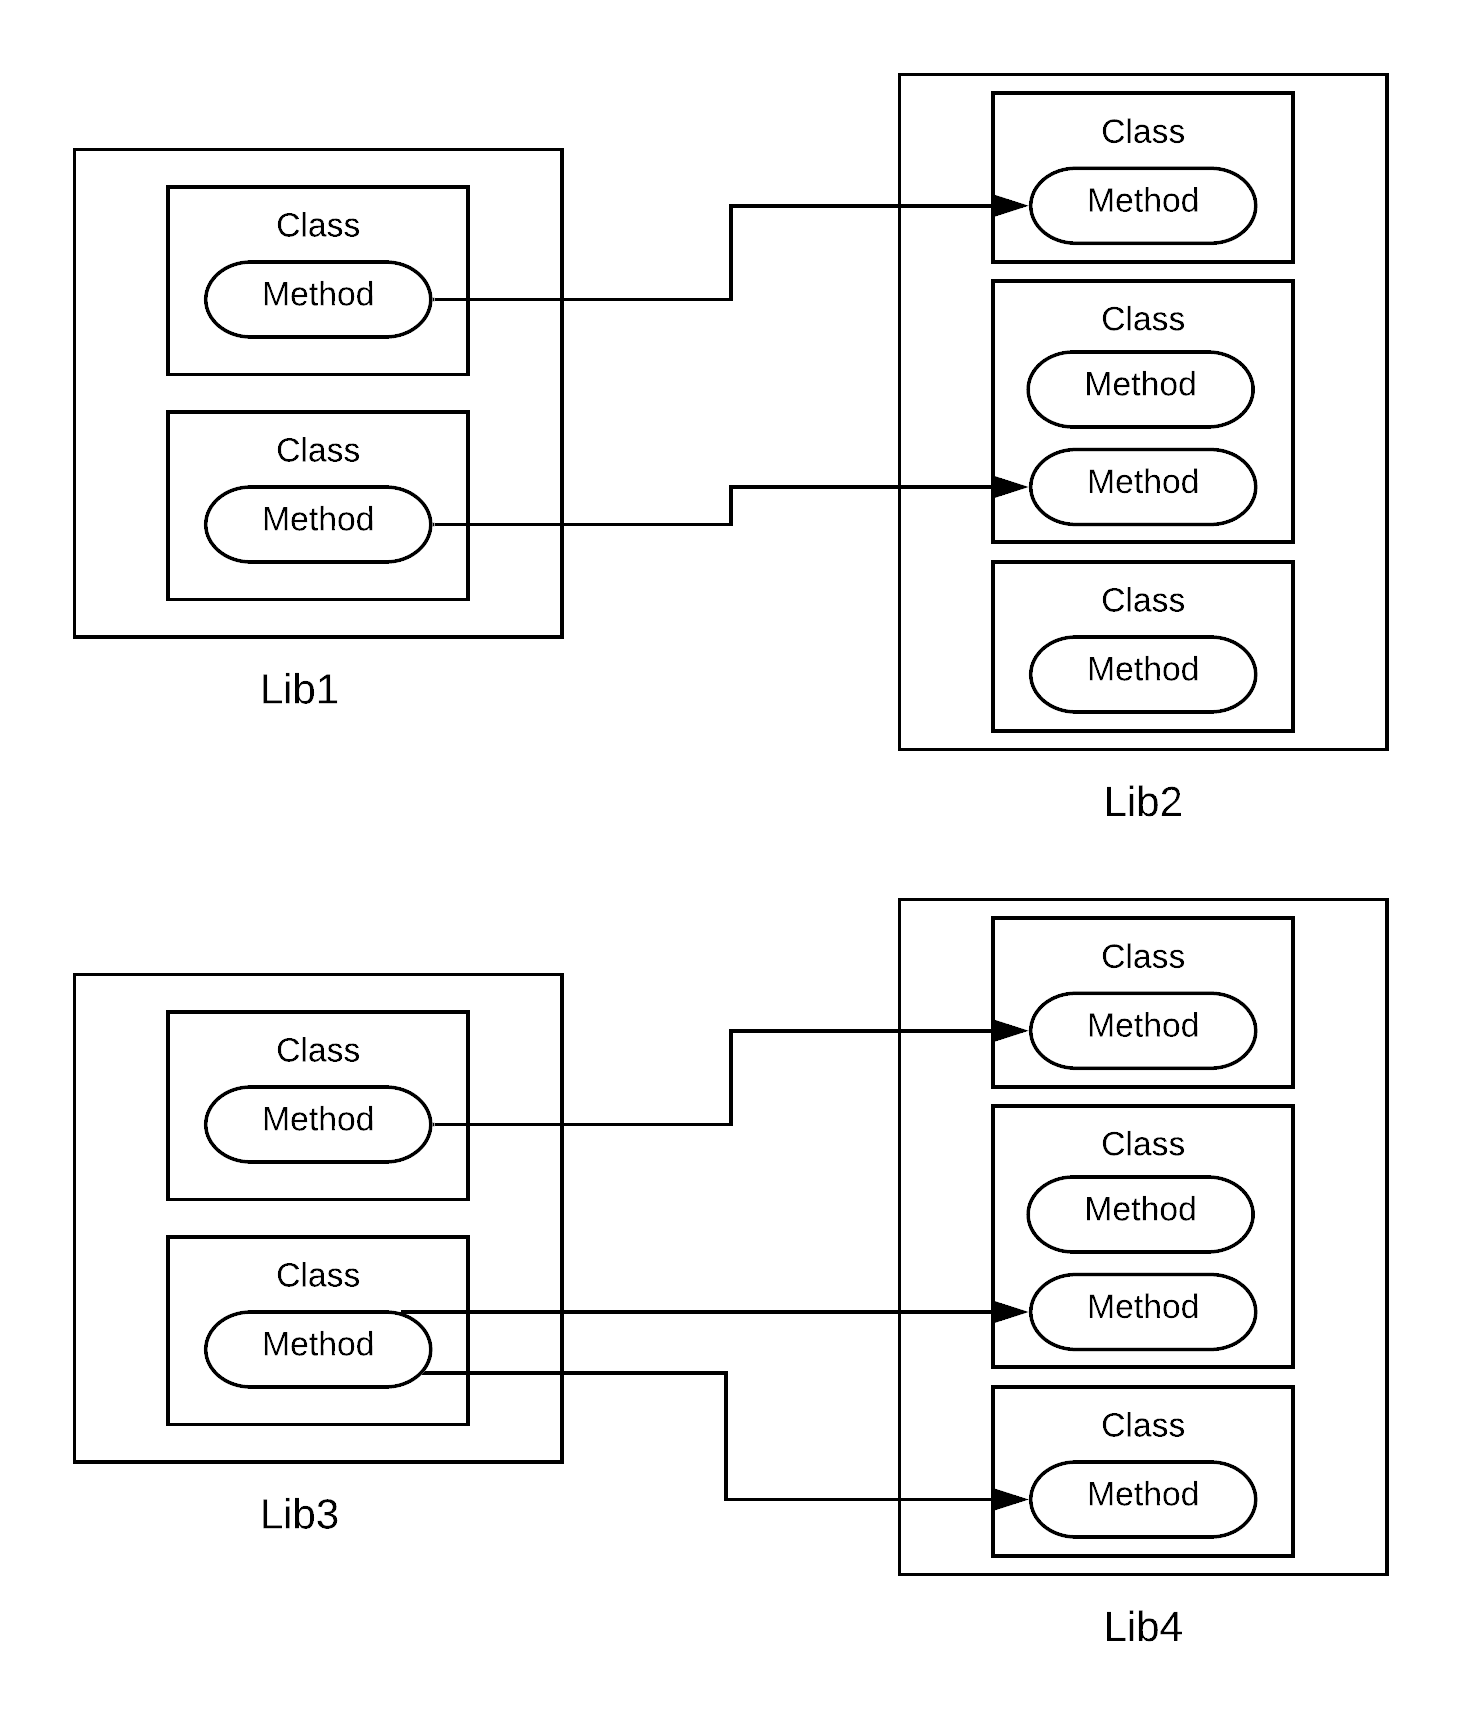
\includegraphics[width=0.7\textwidth]{figures/Example-Percentage-Classes-1.png}
\caption{Example of noncoarseness, percentage of reachable classes}
\label{fig:example-noncoarseness-reachable-classes}
\end{center}
\end{figure}

\paragraph{Property 2: Nonuniqueness}
Following the first example in Figure \ref{fig:example-nonuniqueness-reachable-classes} we take \textit{Lib1} as the client library, and \textit{Lib2} the server library. Therefore, we can see that $|\verb|C|(Lib2)| = 3$, and $|RM(Lib1, Lib2)| = 2$. Hence, calculating the metric using equation \ref{eqn:reachable-classes}, we obtain \(\verb|%ReachableClasses|(Lib1, Lib2) = \frac{2}{3} = 0.66\).

In the second case in Figure \ref{fig:example-noncoarseness-reachable-classes} we have \textit{Lib3} as the client library, and \textit{Lib4} as the server library. Looking at the example, we know that $|\verb|C|(Lib4)| = 3$ and $|RM(Lib3, Lib4)| = 2$. Therefore, the metric for these two libraries is \(\verb|%ReachableClasses|(Lib3, Lib4) = \frac{2}{3} = 0.66\).

Therefore, two different libraries can have the same value for metric \(\verb|%ReachableClasses|\). Hence, the property \textit{Nonuniqueness} holds for this metric.

\begin{figure}[ht]
\begin{center}
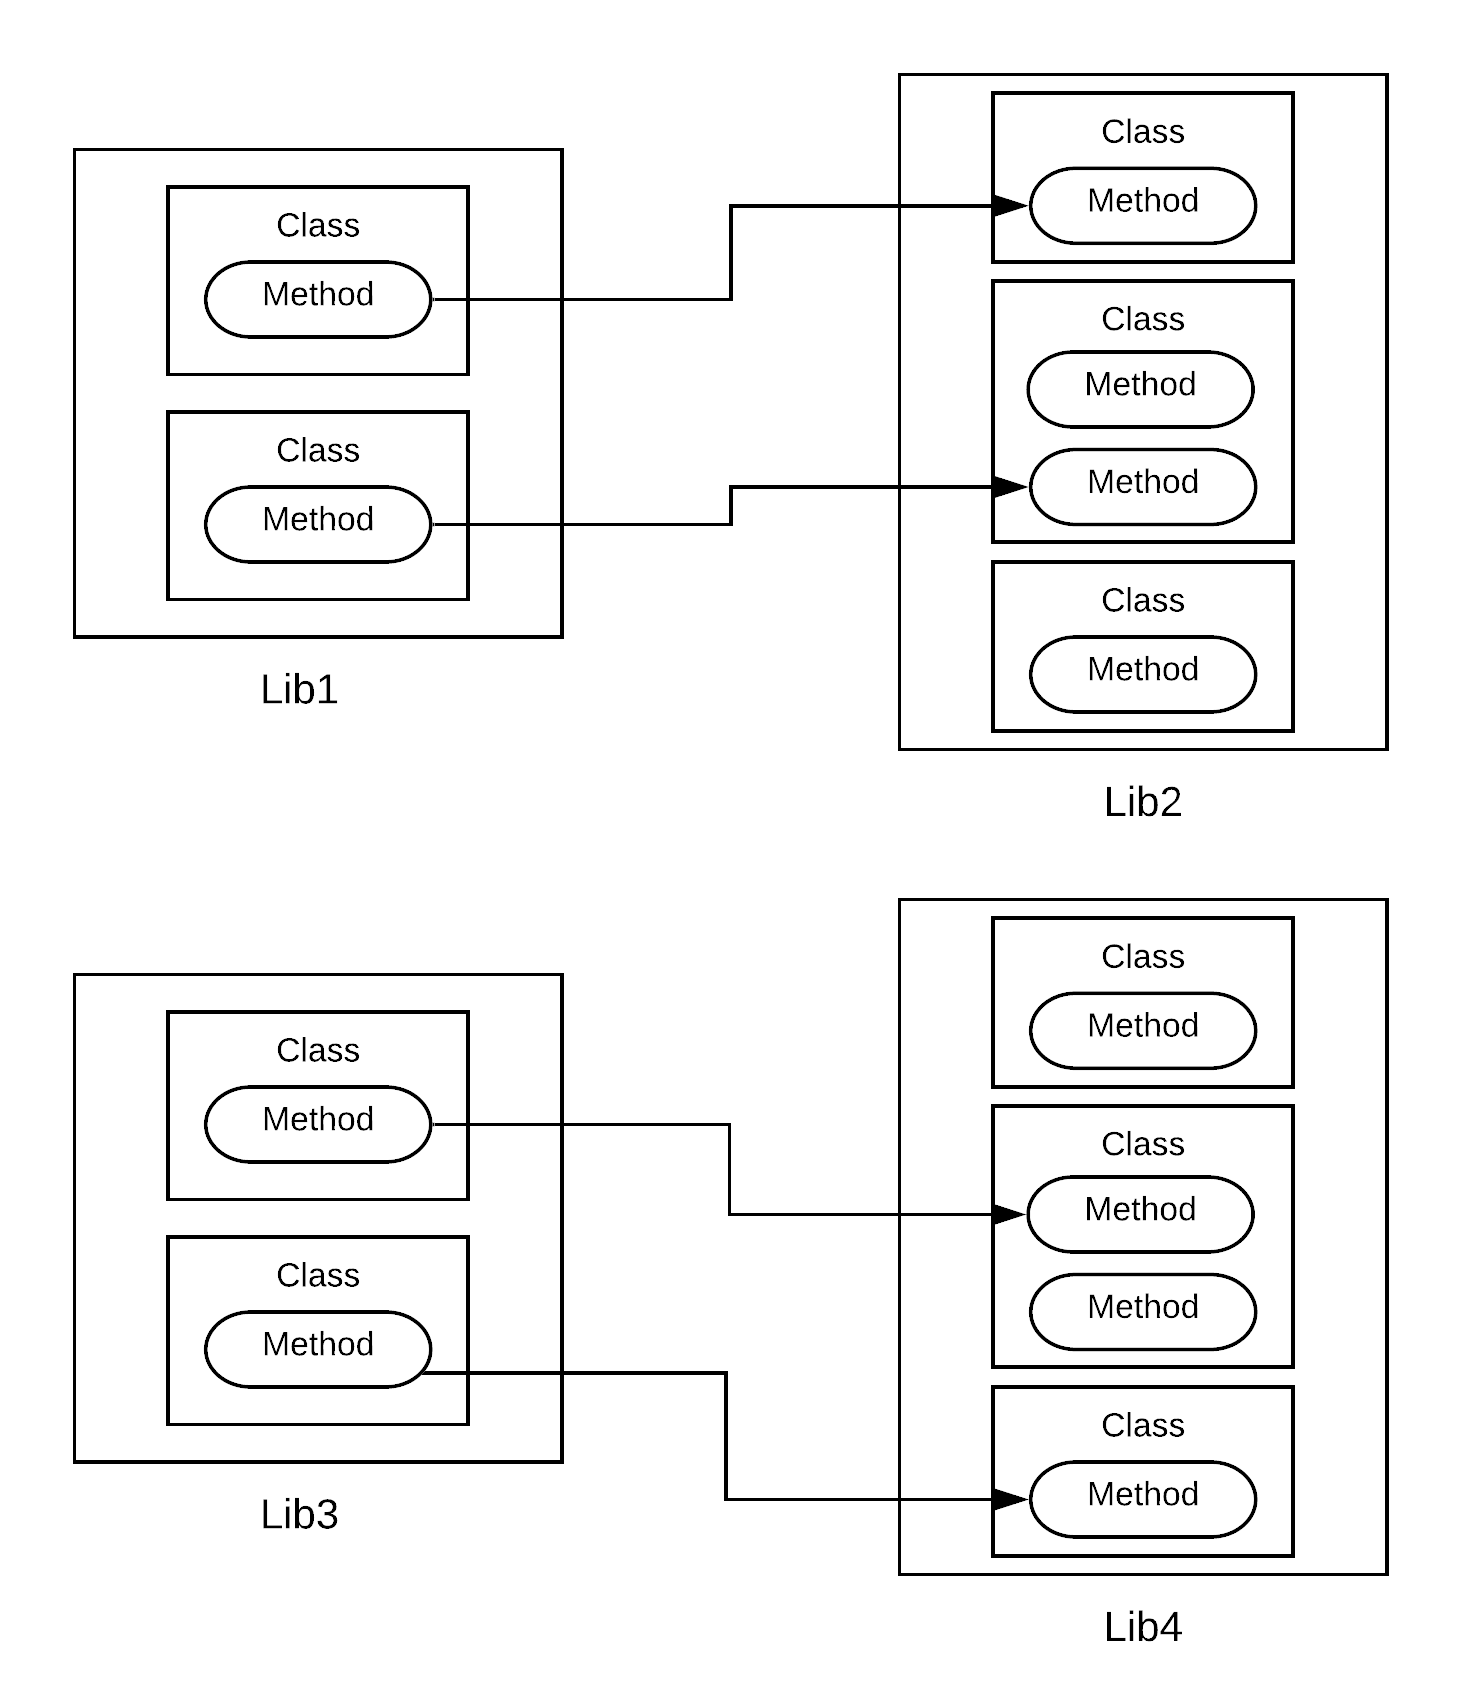
\includegraphics[width=0.7\textwidth]{figures/Example-Percentage-Classes-2.png}
\caption{Example of nonuniqueness, percentage of reachable classes}
\label{fig:example-nonuniqueness-reachable-classes}
\end{center}
\end{figure}

\paragraph{Property 3: Nonnegativity}
Assume that the metric \(\verb|%ReachableClasses|\) does not fulfill this property.
Let $L_c$ be a client library, and $L_s$ be a server library, such that \(\verb|%ReachableClasses|(L_c, L_s) < 0\). Then, we have that $|RC(L_c, L_s)| < 0 \oplus |C(L_s)| < 0$. This means that the cardinality of a set is negative, which is not true by definition. Therefore, it is a contradition.

Hence, the metric fulfills property \textit{Nonnegativity}.

\paragraph{Property 4: Null value}
Let $L_c$ be a client library, and $L_s$ be a server library. There is no usage in $L_c$ of library $L_s$, $RC(L_c, L_s) = \emptyset$. Assuming that the property null value does not hold for \(\verb|%ReachableClasses|\), then \(\verb|%ReachableClasses|(L_c, L_s) \neq 0\). Since this metric has the property nonnegativity, then  \(\verb|%ReachableClasses|(L_c, L_s) > 0\).
Therefore, $\frac{|RC(L_c, L_s)|}{|C(L_s)|} > 0$ and $|RC(L_c, L_s)| > 0$, which contradicts that $RC(L_c, L_s) = \emptyset$.

Therefore, the property \textit{Null value} holds for metric \(\verb|%ReachableClasses|\).

\paragraph{Property 5: Monotonicity}
Having $L_c$ a client library, and $L_s$ a server library. Let $c_c$ be a class in $L_c$, and $c_c'$ a class created as the result of adding more connections to $L_s$ in $c_c$. Then, let $L_c'$ be a client library resulting of replacing $c_c$ by $c_c'$ in $L_c$. Assuming that the property does not hold, we would have that \(\verb|%ReachableClasses|(L_c, L_s) > \verb|%ReachableClasses|(L_c', L_s)\).
Therefore, since $|C(L_s)|$ is the same in both cases because $L_s$ does not change, we have that $|RC(L_c, L_s)| > |RC(L_c', L_s)|$. This means that there is some $c_s$ in $L_s$, which is reachable from $c_c$ and not reachable from $c_c'$. However, $c_c'$ contains all the connections between $c_c$ and $L_s$, and that is therefore not possible.

In conclusion, the metric \(\verb|%ReachableClasses|\) has the property \textit{Monotonicity}.

\section{Measuring impact per class}
\unsure{I'm not sure if impact is really the word I want to use here}
\unsure{Also, I'm not sure about the level of detail needed for these metrics, since it seems pretty simple. Let me know if there is something I should remove or add. Or if I should not treat these as metrics in the same way as the others}

In this case, the goal is to give a bit more low-level information on the impact of the dependency on the client library. It can be useful for a developer or a maintainer to know exactly which the dependency can impact parts of your code. For example, if there is a breaking change, or if the library with a dependency has to be replaced.

This section describes how the impact is measured by these metrics and provides a formal definition of the metrics. Finally, we perform a theoretical validation of the metrics.

\subsection{Definition of impact}
To define the impact to be measured by these metrics, we use the relevant criteria for this case.

\paragraph{Type of connection}
Just as with the coupling metrics, all the types of connection can be relevant, but the impact of each type of connection might be different. Therefore, these should not be measured together. Since this work is meant to be the first approach, we select two possible connection types.

First, the \textit{method invocation}, since it is the only type of connection that refers to the methods used in the dependencies, and therefore is the only one indicating where the server libraries' methods can be invoked from. Then, to represent how the classes of the server libraries are used, and for consistency with the previous metrics, we select the \textit{field declaration}.

\paragraph{Granularity}

As the title of the section indicates, these metrics are measuring the impact \textit{per class}. Hence, the aggregation level of the metric is the \textit{class} level for the client library. In other words, we calculate the metric taking a class of the client library and a server library.

The way the connections are counted for these metrics is not considered in the original list created by Briand et al. \cite{briand1999unified}. Instead, it is counted the number of places of the client class where a connection is originated. For instance, let's take \textit{Lib1} from Figure \ref{fig:example-impact-per-class} as the client library, and \textit{Lib3} as the server library. From \textit{Class1} to \textit{Lib3} there are four different connections, but there are only two origins of these connections. The same happens with \textit{Class2}, in which there are two connections with \textit{Lib3}, but only one origin.

\begin{figure}[ht]
\begin{center}
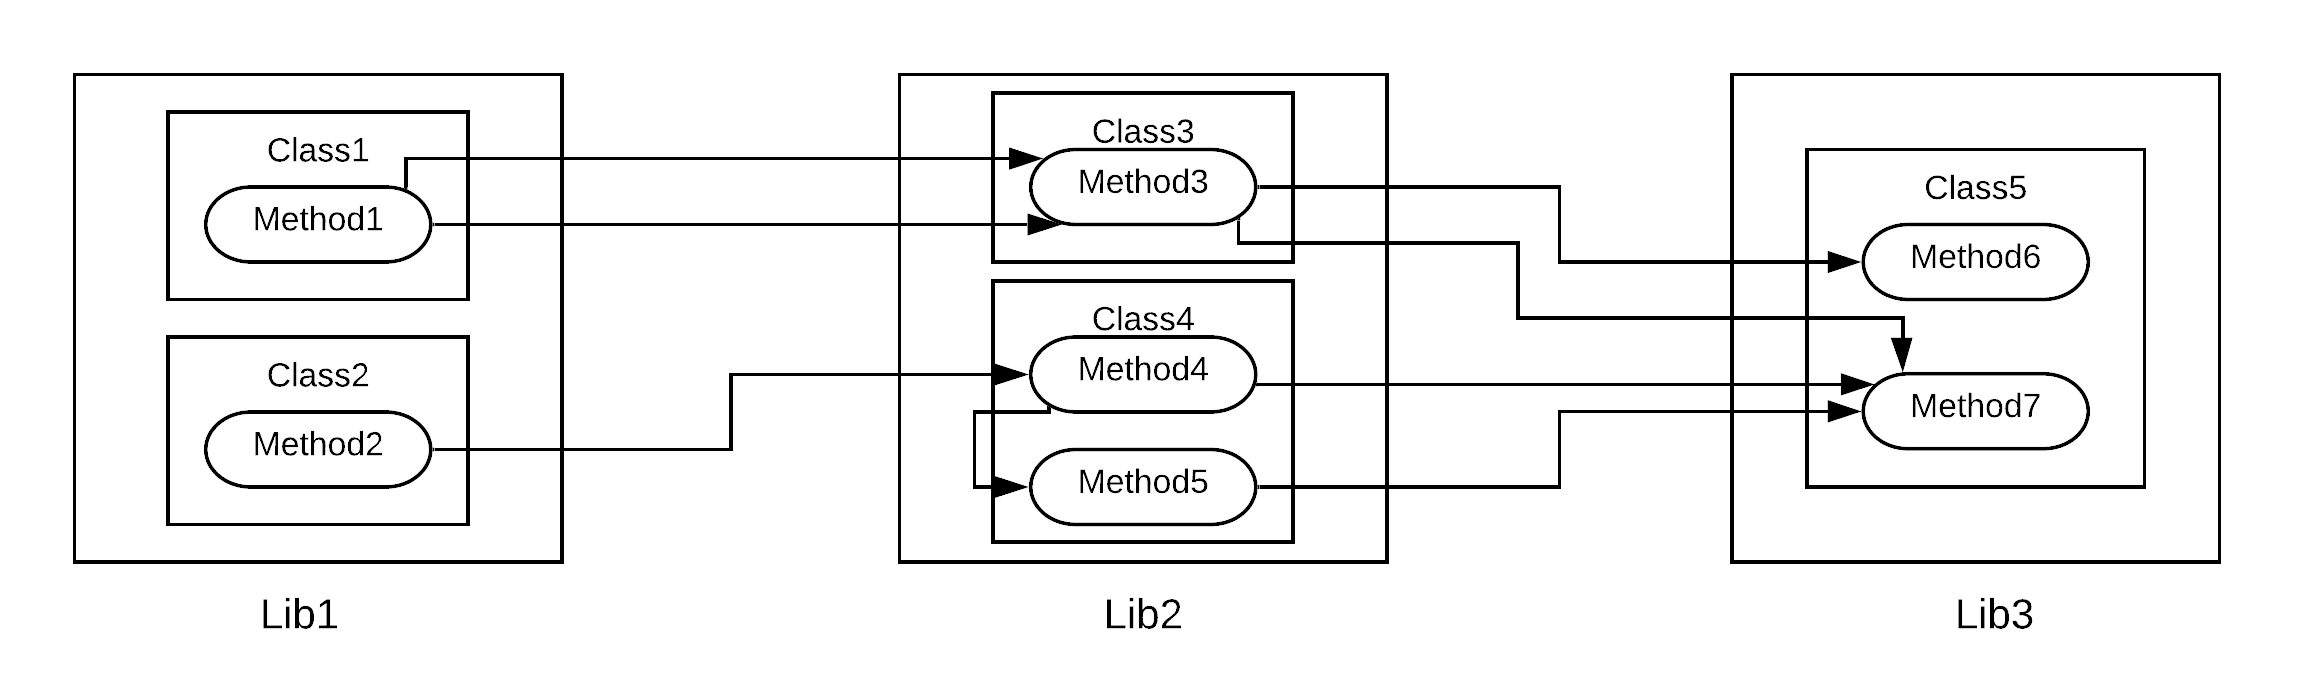
\includegraphics[width=\textwidth]{figures/impact-per-class.png}
\caption{Example to calculate impact per class}
\label{fig:example-impact-per-class}
\end{center}
\end{figure}

\paragraph{Direct \& Indirect}

The connection measured can be either direct or indirect, depending on the dependency between the client and the server library. However, this does not change the calculation of the metric. Hence, both types of dependencies are calculated with the same metric.

\paragraph{Result}
Based on the criteria discussed above, we define two metrics. The summary of the characteristics of these two metrics can be found in Table \ref{table:per-class-characteristics}.

\begin{table}[h]
    \begin{center}
    \begin{tabular}{|l|l|l|l|}
    \hline
    Type of connection & Aggregation level & Counting connections & Direct/Indirect \\ \hline
    Method invocation & Class & \#origin of connection & Both \\
    Field declaration & Class & \#origin of connection & Both \\
    \hline
    \end{tabular}
    \end{center}
    \caption{Criteria of the set of metrics}
    \label{table:per-class-characteristics}
\end{table}

\subsection{Formal definition of the metrics}
\unsure{I am not sure about which names to use here}

\paragraph{Method invocations per class}
Having a client library ($L_c$), and a server library ($L_s$). The result of this metric for a class of the client library ($c_c \in \verb|C|(L_c)$) corresponds to the number of method invocations contained in the methods of $c_c$ ($m_c \in \verb|M|(c_c)$) such that, the call graph created from these method invocations reach a method implemented in the client library ($m_s \in \verb|M|(L_s)$). The set with the method invocations in $m_c$ that reach a method in $L_s$ is $\verb|nIR|(m_c, L_s)$.

\begin{equation}
\label{eqn:mi}
    \verb|#MethodInvocations|(c_c, L_s) =  \sum_{m_c \in \verb|M|(c_c)} |\verb|nIR|(m_c, L_s)|
\end{equation}

\paragraph{Field declaration per class}
This metric is calculated in the following manner. For a class $c_c$ of a client library $L_c$ ($c_c \in \verb|C|(L_c)$), and a server library $L_s$. The result of the metric for $c_c$, corresponds to the number of field declarations in $c_c$ such that, through field declarations reach a class implemented in $L_s$. The set of field declarations that reach $L_s$ is denoted $\verb|nFR|(c_c, L_s)$.

\begin{equation}
\label{eqn:fd}
    \verb|#FieldDeclarations|(c_c, L_s) = |\verb|nFR|(c_c, L_s)|
\end{equation}

\subsection{Theoretical validation}
This section contains the proofs, for the metrics $\verb|#MethodInvocations|$ and $\verb|#FieldDeclarations|$, of the properties that these should have. The proofs are done for one metric since they can be done for the other metric very similarly.

The properties chosen in this case are the same as the ones chosen in Section \ref{subsect:theoretical-validation-usage} since these properties can also be applied for these metrics. Nevertheless, the description of the properties has been adapted to fit the characteristics of the metrics.

\begin{enumerate}
  \item \textbf{Noncoarseness:} Two different classes can have different values for the same metric.
  \item \textbf{Nonuniqueness:} There can exist different classes with the same value.
  \item \textbf{Nonnegativity:} The value of the metric should never be negative.
  \item \textbf{Null value:} The value of the metric is expected to be zero if there is no connection of the type measured by the metric from the client class to the server library.
  \item \textbf{Monotonicity:} It is expected that if more usage is added from the client class to the server library, the metric value does not decrease.
\end{enumerate}

\paragraph{Property 1: Noncoarseness}
Following the first case in Figure \ref{fig:example-noncoarseness-method-invocation}, we take textit{Lib1} as the client library, \textit{Lib2} as the server library, and the only class in \textit{Lib1} as $c_c$. We can see that the class has only one method, for which $|\verb|nIR|(Method, Lib2)| = 1$. Therefore, following the equation \ref{eqn:mi}, we have that $\verb|#MethodInvocations|(c_c, Lib2) = 1$.

Now we move to the second case in Figure \ref{fig:example-noncoarseness-method-invocation}. In this case we take \textit{Lib3} as the client library, \textit{Lib4} as the server library, and the class in \textit{Lib3} as $c_c$. $c_c$ has only one method, for which $|\verb|nIR|(Method, Lib4)| = 3$. Hence, $\verb|#MethodInvocations|(c_c, Lib4) = 3$.

In conclusion, two different classes can have different values for metric $\verb|#MethodInvocations|$, which fulfills property \textit{Noncoarseness}.

\begin{figure}[ht]
\begin{center}
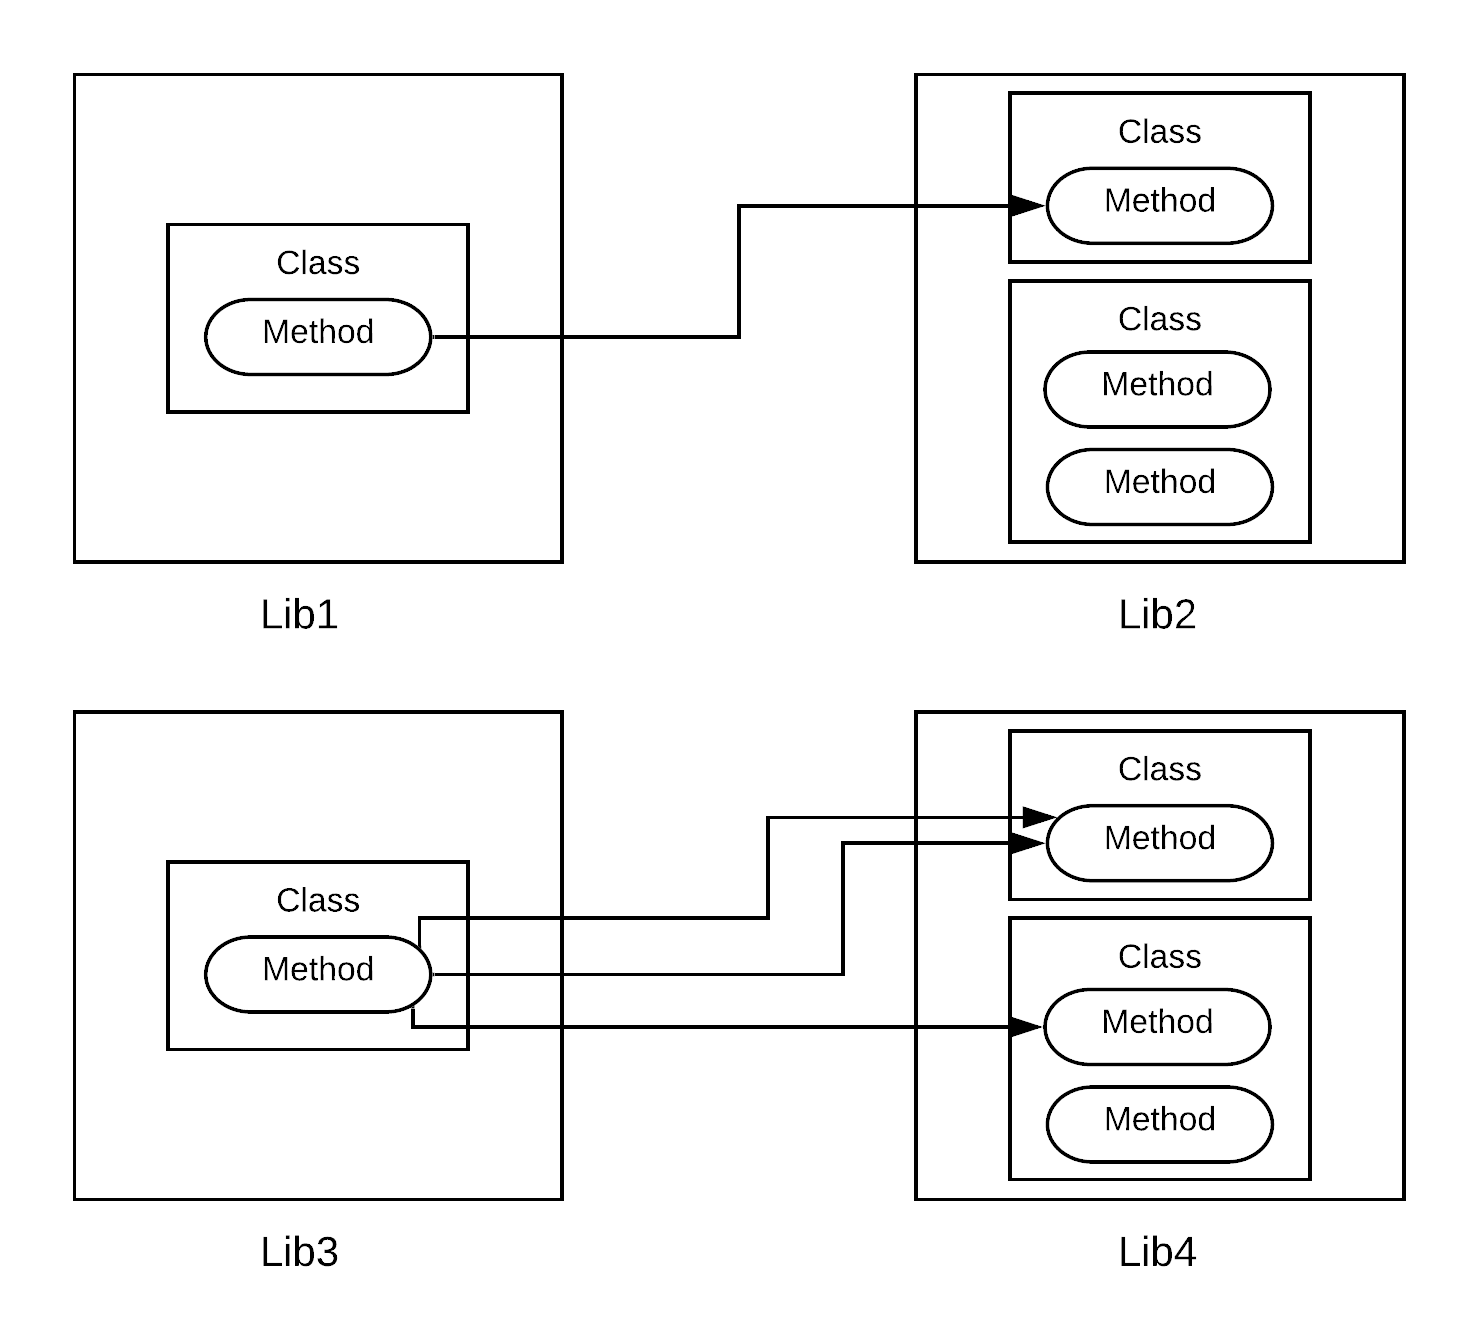
\includegraphics[width=0.7\textwidth]{figures/Example-Distribution-1.png}
\caption{Example of noncoarseness, number of method invocations}
\label{fig:example-noncoarseness-method-invocation}
\end{center}
\end{figure}

\paragraph{Property 2: Nonuniqueness}
Now we look at Figure \ref{fig:example-nonuniqueness-method-invocation}, and in the first example we take \textit{Lib1} as the client library, \textit{Lib2} the server library, and the class in \textit{Lib1} as the client class, $c_c$. The client class has only one method, for which $|\verb|nIR|(Method, Lib2)| = 2$. Therefore, the value of the metric in this case, is as follows, $\verb|#MethodInvocations|(c_c, Lib2) = 2$.

Focusing on the second case in Figure \ref{fig:example-nonuniqueness-method-invocation}, we have that \textit{Lib3} is the client library and \textit{Lib4} the server library. Also, the client class, $c_c$, is the only class in \textit{Lib3}. We can see that there is one method in $c_c$, which calls \textit{Lib4} a total of 2 times, $|\verb|nIR|(Method, Lib4)| = 2$. Hence, $\verb|#MethodInvocations|(c_c, Lib4) = 2$.

With this example, we see that two different classes can have the same value for $\verb|#MethodInvocations|$. Therefore, this metric fulfills the property \textit{Nonuniqueness}.

\begin{figure}[ht]
\begin{center}
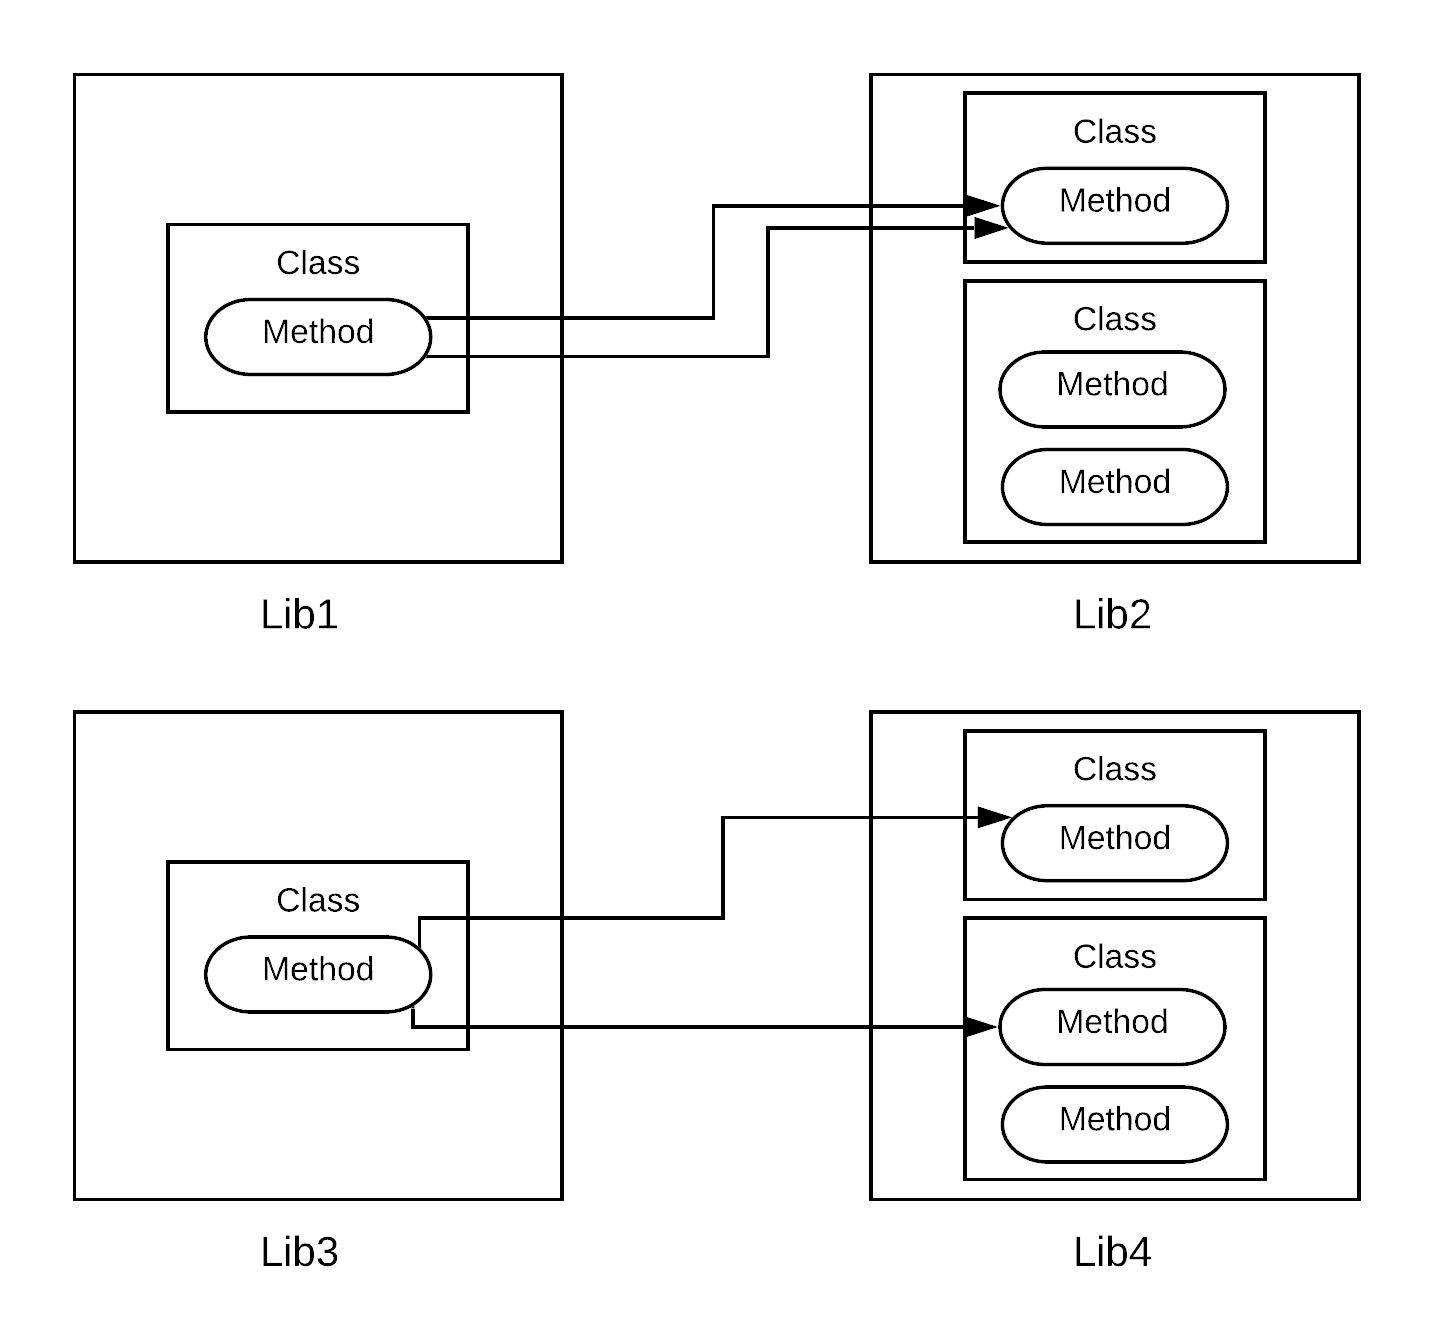
\includegraphics[width=0.7\textwidth]{figures/Example-Distribution-2.png}
\caption{Example of nonuniqueness, number of method invocations}
\label{fig:example-nonuniqueness-method-invocation}
\end{center}
\end{figure}

\paragraph{Property 3: Nonnegativity}
If the property does not hold for $\verb|#MethodInvocations|$, there exists a client library $L_c$ containing $c_c$ and a server library $L_s$, such that $\verb|#MethodInvocations|(c_c, L_s)
< 0$. Therefore, exsists a method $m_c \in \verb|M|(c_c)$, such that $|\verb|nIR|(m_c, L_s)| < 0$. However, the cardinality of a set cannot be negative by definition, and therefore it is a contradition.

Hence, the property \textit{Nonnegativity} holds for metric $\verb|#MethodInvocations|$.

\paragraph{Property 4: Null value}
Assume that the metric does not fulfill property null value. Let $L_c$ and $L_s$ be a client library and a server library, adn $c_c$ a class in $L_c$. Assume that $c_c$ does not have any connection to $L_s$, and given that the metric does not fulfill \textit{null value}, $\verb|#MethodInvocations|(c_c, L_s) \neq 0$. From the previous proof we know that $\verb|#MethodInvocations|(c_c, L_s) \geq 0$, then  $\verb|#MethodInvocations|(c_c, L_s) > 0$.
Hence, there is a method $m_c \in \verb|M|(c_c)$ such that $|\verb|nIR|(m_c, L_s)| > 0$. Since $\verb|nIR|(m_c, L_s)$ is the set of method invocations in $c_c$ that reach $L_s$, there has to be a connection between $c_c$ and $L_s$, which constitutes a contradition.

Therefore, the metric fulfills property \textit{Null value}.

\paragraph{Property 5: Monotonicity}
Let $L_c$ be a client library, and let $L_s$ be a server library. Given a class $c_c$ in $L_c$, we define $c_c'$ as a copy $c_c$ with added connections to $L_s$. Let $L_c'$ be a client library identical to $L_c$,. but in which $c_c$ has been replaced by $c_c'$. Assume that metric $\verb|#MethodInvocations|$ does not fulfill \textit{Monotonicity}. Therefore, $\verb|#MethodInvocations|(c_c, L_s) > \verb|#MethodInvocations|(c_c, L_s)$.
Then, for a given $m_c \in \verb|M|(c_c)$, and its copy in $c_c'$, $m_c' \in \verb|M|(c_c')$, such that $|\verb|nIR|(m_c, L_s)| > |\verb|nIR|(m_c', L_s)|$. This means that $m_c$ contains a method invocation which reaches $L_s$ and it is not included in $m_c'$. However, all the method invocations contained in $c_c$ are maintained in $c_c'$. Therefore, it is a contradition.

Hence, property \textit{Monotonicity} holds for metric $\verb|#MethodInvocations|$.

\newpage
% !TEX root = ../main.tex
\chapter{Proof of Concept}\label{ch:PoC}
In this section we describe the different parts of the proof-of-concept implementation of the model. First, we discuss the possible techniques to implement it, and describe the chosen one. Then, there is an explanation of how each one of the metrics is measured, including pseudo-code to illustrate it.

\section{Analysis technique}
There are several techniques that could have been used to implement the PoC that calculates the different metrics proposed.

\begin{itemize}
  \item Bytecode analysis
  \item Source code analysis
  \item Call-level dependency graph
\end{itemize}

After an initial try, source code analysis has been discarded. The reason for it is that the source code is needed for both the client library, and all its dependencies. Although, it is sometimes available in Maven, it is not available as often as the bytecode.

The option of call-level dependency graphs is useful for the metrics that measure method invocations. However, the information needed to measure aggregation coupling, is not contained in the call-level graphs. Therefore, the approach to develop this PoC has been bytecode analysis. Furthermore, obtaining the call-graphs of the complete dependency tree is still a work in progres within the FASTEN project.

\subsection{Bytecode analysis}
The model proposed in this research is meant to be language-agnostic. Nevertheless, the scope of the proof-of-concept is limited to Java, since the bytecode analysis performed by the proof-of-concept is limited to this programming language. Furthermore, the PoC is focused on the libraries available in Maven.

The PoC implementation is supported by the libraries  \textit{Aether}\footnote{\url{https://wiki.eclipse.org/Aether/What_Is_Aether}}, and \textit{Javassist}\footnote{\url{http://www.javassist.org/}}.

\paragraph{Aether}
Aether is a library created by Eclipse, which allows to fetch Maven artifacts from different repositories. In addition, it is also used to resolve the dependencies of a library, and create the dependency tree. To create the dependency tree, Aether uses the same strategy to resolve the dependencies as Maven.

In the PoC, this library has been used for the initial steps. The request to calculate the metrics receives the identifiers of the library to analyze (\textit{GroupId}, \textit{ArtifactId}, and \textit{version}). Aether is used to fetch the library \textit{jar} and \textit{POM} files from the Maven Central Repository.

Once the artifact of the client library is obtained, \textit{Aether} is used to resolve the dependencies of the artifact. For the calculation of the metrics to be possible, all the dependencies of the client library should also be available in the Maven Central Repository. The dependency tree of the artifact is visited, and each of the dependencies are also obtained, in order to have the \textit{jar} files to analyze as well. In addition, the dependency tree calculated with Aether is also used to create a custom dependency tree by using the custom class \texttt{DependencyTreeNode} which stores the data about each of the libraries which is needed during the process of calculating the metrics. The \texttt{DependencyTreeNode} will be described in greater detail later on.

\paragraph{Javassist}
Javassist is a library which allows the used to perform bytecode manipulation in a simple way. It has two levels, a source-level and a bytecode level. By using the source-code level, it is possible to perform bytecode analysis and manipulation without a deep knowledge of bytecode. Meanwhile, the bytecode level allows the user to directly manipulate bytecode.
For this thesis, the level used is source-code.

The javassist library has been used to interpret and analyze the jars of the client library and all the server libraries. Once the jars of the client library and all its dependencies are available, the first step is to join all the \textit{.class} files in a \texttt{ClassPool} object, which is the main object of \textit{Javassist}. Once the \texttt{ClassPool} is created, it is used to obtain the classes from the client library, from which the different metrics are calculated. The process of calculating the metrics is explained in greater detail in the following

\subsection{Model of the dependency tree}
In order to represent the dependency tree of the client library, the implementation uses the class \texttt{DependencyTreeNode}. Each \texttt{DependencyTreeNode} contains the information of the library it represents, namely \textit{groupID}, \textit{artifactID}, and \textit{version}. Also, to represent the dependencies of the library represented by each  \texttt{DependencyTreeNode}, there is a \texttt{List} of \texttt{DependencyTreeNode}.

To store the information needed to calculate the coupling metrics, there are two other classes: \texttt{MicBehaviors}, \texttt{AcClasses}, for \texttt{MIC} and \texttt{AC} respectively. \texttt{MicBehaviors} is a map, containing for each method or constructor (behavior) of the server library used to calculate \texttt{MIC}, a \texttt{Set} with all the method calls from which it is reachable. In the same way, \texttt{AcClasses} is a map, in which for each class of a server library used to calculate \texttt{AC}, there is a \texttt{Set} of all the field declarations from which the class is reachable. The behaviors and classes used to calculate \texttt{MIC} and \texttt{AC} are those which are reachable through the type of connection of the metric.

Each \texttt{DependencyTreeNode} has an object \texttt{MicBehaviors} and \texttt{AcClasses} for each of the distances at which the metric is measured, stored as a map, where the distance is the key and \texttt{MicBehaviors} or \texttt{AcClasses}, the value.

In addition, for the metrics that measure the usage of the dependencies, there are two other fields: \texttt{ReachableClasses} and \texttt{ReachableBehaviors}. The first field is to calculate the \(\verb|%ReachableClasses|\), and the second one for \(\verb|%ReachableMethods|\). Both, \texttt{ReachableClasses} and \texttt{ReachableBehaviors}, are sets containing the classes, in the first case, and behaviors in the second case, of the library represented by the \texttt{DependencyTreeNode}, which are reachable from the client library.

\begin{figure}[ht]
\begin{center}
\includegraphics[width=\textwidth]{figures/Thesis-ModelClassDiagram.png}
\caption{Class diagram, dependency tree model}
\label{fig:class-diagram-tree}
\end{center}
\end{figure}

\section{Measuring coupling metrics}
This section contains the description of how the metrics \texttt{MIC}, \texttt{AC}, \texttt{TMIC}, and \texttt{TAC} are calculated in the implementation of the PoC. During this section, we use the terminology of the library Javassist. For example, to refer to methods and constructors, we say behaviors. Also, the classes used from Javassist are named as \texttt{Ct<name of the element>}, where \texttt{Ct} means compile-time. Therefore, the class representing a java class is \texttt{CtClass}.

\subsection{Method Invocation Coupling}
The pseudo-code in Figure \ref{fig:algorithm-mic} represents the algorithm used to calculate the metric \textit{MIC} for each one of the direct dependencies of a given client library. The output of the algorithm is a map containing the set of \texttt{BehaviorCalls} that call each \texttt{CtBehavior}. The map is generated for each one of the direct dependencies and stored in the \texttt{DependencyTreeNode} of each library.

The class \texttt{CtBehavior} contains the information about the behavior itself, and about the class in which it is declared. Each of the \texttt{CtBehavior} are used later on to find the polymorphic implementations of the behavior, as well as to calculate the metrics for the transitive dependencies.

To calculate this first metric, the implementation iterates through all the classes of the client library (line 3). For each class, the behaviors are obtained (line 4).

Then, the tool iterates through all the behaviors (line 5), and calls the method \texttt{instrument}. The main use case of this method is to modify the bytecode of the method, but in this case we use it to find the connections of interest for this metric. The method \texttt{instrument} receives an \texttt{ExprEditor} object, which is a class that can be extended to implement the methods for editing the bytecode, which are empty by default. To calculate this metric, the overridden methods are \texttt{edit(MethodCall mc)}, \texttt{edit(ConstructorCall cc)}, and \texttt{edit(NewExpr ne)}. These methods will be called for each method call or constructor call, existing in the bytecode of the method (line 6). The constructor calls in the form of \texttt{this()} or \texttt{super()} are captured by the method \texttt{edit(ConstructorCall cc)}. Meanwhile, the constructor calls in the form of \texttt{new Object()} are captured by \texttt{edit(NewExpr ne)}.

For each captured call to a behavior, it is checked if the called behavior belongs to a server library (line 9). In case it does, the call is added to the \texttt{MicBehaviors} map of the server library (line 10), with 1 as the distance at which the connection is found, since it is a direct dependency.

\begin{figure}[ht!]
\begin{lstlisting}[escapeinside={(*}{*)}]
clientClasses = classPoolManager.getClientLibraryClasses()

for each clientClass in clientClasses
  behaviors = clientClass.getDeclaredBehaviors()
  for each behavior in behaviors
    for each behaviorCall in behavior
      serverBehavior = behaviorCall.getBehavior()
      serverClass = serverBehavior.getDeclaringClass()
      if (classPoolManager.belongsToClientLibrary(serverClass))
        dependencyTreeNode.addMicBehavior(serverBehavior, behaviorCall, distance = 1)
\end{lstlisting}
\caption{Pseudo-code of the algorithm to calculate MIC}
\label{fig:algorithm-mic}
\end{figure}

\subsection{Aggregation Coupling}
The pseudo-code in Figure \ref{fig:algorithm-ac} represents the algorithm used to calculate the metric \texttt{AC}. The output of the algorithm is a map containing for each \texttt{CtClass} of the server library, the set of \texttt{CtField} that are of the type of the \texttt{CtClass}. The class \texttt{CtClass} represents a class and contains the information about the class itself and about the library where it is implemented. \texttt{CtClass} is used later on to find the descendants of the class, and to calculate the metric \texttt{TAC} for the transitive dependencies.

The algorithm for this second metric is similar to the previous one. The implementation iterates through all the classes of the client library (line 3). Then, for each class, it iterates through all the declared fields (line 5). Next, each of the fields containing a generic type are parsed separatedly (line 6), to obtain all the types icluded in the generic (line 7), which are treated individually (line 8). All the simple fields, if the implementation of the class is found in a server library (line 13), are included in the calculation of the metric (line 14). The distance is set to 1 due to the server library being a direct dependency.

\begin{figure}[ht!]
\begin{lstlisting}[escapeinside={(*}{*)}]
clientClasses = classPoolManager.getClientLibraryClasses()

for each c in clientClasses
  fields = c.getDeclaredFields()
  for each field in fields
    if (field.containsGeneric())
      serverClasses = getAllClasses(field)
      for each serverClass in serverClasses
        if (classPoolManager.belongsToClientLibrary(serverClass))
          dependencyTreeNode.addAcClass(serverClass, field)
    else
      serverClass = field.getType()
      if (classPoolManager.belongsToClientLibrary(serverClass))
        dependencyTreeNode.addAcClass(serverClass, field, distance = 1)
\end{lstlisting}
\caption{Pseudo-code of the algorithm to calculate AC}
\label{fig:algorithm-ac}
\end{figure}

\paragraph{Inheritance}\label{paragraph:inheritance}
Once the two algorithms (Figures \ref{fig:algorithm-mic} and \ref{fig:algorithm-ac}) are finished, in order to follow the definition of the metrics as specified in section \ref{subsec:metric-definition} the hierarchies in the server libraries are visited. For the metric \texttt{MIC} all the polymorphic implementations of the behaviors are found, and for the metric \texttt{AC} all the descendants of the classes.

The algorithms to find the descendants and the polymorphic implementations of the methods, are used with each one of the libraries with which the client library has a direct dependency, and for which coupling was found, either \texttt{MIC} or \texttt{AC}.

The pseudo-code used to find the polymorphic implementations of the methods can be found in Figure \ref{fig:algorithm-polymorphy}. The process is as follows: First, iterate through all the classes of the server library, given its \texttt{DependencyTreeNode} (line 5). Then, it iterates through the behaviors in the map contained in \texttt{MicBehaviors}. If the current library class is a descendant of the class containing the reachable behavior (line 8), and it contains a behavior with the same signature as the reachable behavior (line 9), a polymorphic implementation of the behavior has been found. Therefore, the found behavior is added to the \texttt{MicBehaviors} with the same set of \texttt{BehaviorCall} and distance as the mic behavior (line 11).

\begin{figure}[ht!]
\begin{lstlisting}[escapeinside={(*}{*)}]
serverLibrary = dependencyTreeNode.getLibrary()
micBehaviorsMap = dependencyTreeNode.getMicBehaviors()
serverLibraryClasses = classPoolManager.getLibraryClasses(serverLibrary)

for each serverClass in serverLibraryClasses
  for each micBehavior in micBehaviorsMap
    declaringClass = micBehavior.getDeclaringClass()
    if (serverClass.isSubClassOf(declaringClass))
      if (serverClass.containsBehavior(micBehavior.getSignature()))
        serverBehavior = serverClass.getBehavior(reachableBehavior.getSignature())
        dependencyTreeNode.addMicBehavior(serverBehavior, micBehavior.getBehaviorCalls(), distance)
\end{lstlisting}
\caption{Pseudo-code of the algorithm to find polymorphic implementations}
\label{fig:algorithm-polymorphy}
\end{figure}

The process to find descendants in the case of the metric \texttt{AC} is the same as the one in Figure \ref{fig:algorithm-polymorphy}, but iterating over the \texttt{reachableClassesMap} instead of the \texttt{reachableBehaviorsMap}. Therefore, if the server class is sub-class of a reachable class, it is added to the \texttt{AcClasses} of the library.

\blankl
As can be observed in the previous explanation of how the detection of inheritance is done, in this PoC implementation, it is not detected if a class is extended in the client library instead of in the server library.\todo{Find out how often does this happen}

\subsection{Transitive Method Invocation Coupling}\label{subsec:tmic}
The calculation of \texttt{TMIC} takes place after calculating \texttt{MIC} for all the direct dependencies of the client library. The methods used in the calculation of \texttt{MIC} from these dependencies, are used as a base to calculate \texttt{TMIC}.

To calculate the metric for every dependency in the tree, the dependency tree is traversed using a \textit{breadth-first search (BFS)} on the \texttt{DependencyTreeNode}. The algorithm starts with the direct dependencies, since the client library node has already been used for the calculation of \texttt{MIC}. The traversing of a branch finishes either when a node does not have more children, or when no reachable methods have been found in a server library. The pseudo-code of the implemented algorithm can be found in Figure \ref{fig:tree-traversing-tmic}.

For each \texttt{DependencyTreeNode} visited, the method \texttt{calculateTransitiveMIC} is executed. The pseudo-code of this method can be found in Figure \ref{fig:calculate-tmic}, which is going to be explained below.

\begin{figure}[ht!]
\begin{lstlisting}[escapeinside={(*}{*)}]
toVisit = queue(clientLibraryNode.getChildren())

while (!toVisit.isEmpty())
  visiting = toVisit.poll()
  if (visiting.hasMicBehaviors())
    findPolymorphicImplementations(visiting.getMicBehaviors())
    if (visiting.hasChildren())
      calculateTransitiveMIC(visiting)
      toVisit.add(visiting.getChildren())
\end{lstlisting}
\caption{Pseudo-code of the \textit{BFS} used for \texttt{TMIC}}
\label{fig:tree-traversing-tmic}
\end{figure}

\begin{figure}[ht!]
\begin{lstlisting}[escapeinside={(*}{*)}]
micBehaviors = visitingTreeNode.getMicBehaviors()

for each micBehavior in micBehaviors
  behaviorsToVisit = queue(micBehavior)
  visitedBehaviors = (*$\emptyset$*)
  while (!behaviorsToVisit.isEmpty())
    visitingBehavior = behaviorsToVisit.poll()
    if (visitedBehaviors.contains(visitingBehavior)) continue
    visitedBehaviors.add(visitingBehavior)

    for each behaviorCall in visitingBehavior
      calledBehavior = behaviorCall.getBehavior()
      calledClass = calledBehavior.getDeclaringClass()
      if (classPoolManager.isStandardClass(calledClass))
        continue
      else if (classPoolManager.isClassInDependency(calledClass, visitingLibrary))
        visitingLibrary.addMicBehaviorToDependency(calledClass, distance + 1)
      else // calledClass is in current library
        behaviorsToVisit.add(calledBehavior)
\end{lstlisting}
\caption{Pseudo-code of the algorithm to calculate \texttt{TMIC}}
\label{fig:calculate-tmic}
\end{figure}

First, we obtain all the behaviors of the visited \texttt{DependencyTreeNode}, used for the calculation of \texttt{MIC} (line 1). For each one of these behaviors (line 3), the call graph of the behavior is iterated, to find all the reachable behaviors of the dependencies of the library that is being visited.

A queue of the behaviors that have to be visited is created, containing initially only the current behavior (line 4). In addition, a set of all the behaviors that have already been visited is also created (line 5) to avoid infinite loops.

For each behavior in the queue, all the \texttt{behaviorCall} are visited (line 11). Then, there are three different cases to consider. First, if the called behavior is implemented in a standard class the call is ignored (line 14). Also, if the called behavior is implemented in a dependency of the current library, the behavior is added to the behaviors to consider of the dependency (line 16), with the same distance plus 1, since it is one level more of dependency than the current \texttt{DependencyTreeNode}. Finally, the last option is if the called behavior is implemented in the current library, in which case it is added to the queue of behaviors to visit (line 19). This way the entire call graph of the relevant behaviors is visited.

\subsection{Transitive Aggregation Coupling}
The calculation of \texttt{TAC} is very similar to the calculation of \texttt{TMIC} but using the ac classes instead of the mic behaviors. The pseudo-code of the \textit{BFS} for the \texttt{TAC} is in Figure \ref{fig:tree-traversing-tac}.

\begin{figure}[ht!]
\begin{lstlisting}[escapeinside={(*}{*)}]
toVisit = queue(clientLibraryNode.getChildren())

while (!toVisit.isEmpty())
  visiting = toVisit.poll()
  if (visiting.hasAcClasses())
    findDescendants(visiting.getAcClasses())
    if (visiting.hasChildren())
      calculateTransitiveAC(visiting)
      toVisit.add(visiting.getChildren())
\end{lstlisting}
\caption{Pseudo-code of the \textit{BFS} used for \texttt{TAC}}
\label{fig:tree-traversing-tac}
\end{figure}

The implementation of the method \texttt{calculateTransitiveAC} also follows a similar strategy as the \texttt{calculateTransitiveMIC}, but instead of iterating the call grpahs of the reachable methods, it iterates the field declarations of the classes. The pseudo-code can be found in Figure \ref{fig:calculate-tac}.

\begin{figure}[ht!]
\begin{lstlisting}[escapeinside={(*}{*)}]
acClasses = visitingTreeNode.getAcClasses()

for each acClass in acClasses
  classesToVisit = queue(acClass)
  visitedClasses = (*$\emptyset$*)
  while (!classesToVisit.isEmpty())
    visitingClass = classesToVisit.poll()
    if (visitedClasses.contains(visitingClass)) continue
    visitedClasses.add(visitingClass)

    fields = visitingClass.getDeclaredFields()
    for each field in fields
      if (field.containsGeneric())
        classesInField = getAllClasses(field)
        for each classInField in classesInFIeld
          if (classPoolManager.isStandardClass(classInField)) continue
          else if (classPoolManager.isClassInDependency(classInField, visitingLibrary))
            visitingLibrary.addAcClassToDependency(classInField)
          else // classInField is in current library
            classesToVisit.add(classInField)
      else
        classInField = field.getType()
        if (classPoolManager.isStandardClass(classInField)) continue
        else if (classPoolManager.isClassInDependency(classInField, visitingLibrary))
          visitingLibrary.addReachableClassToDependency(classInField, distance + 1)
        else // classInField is in current library
          classesToVisit.add(classInField)
\end{lstlisting}
\caption{Pseudo-code of the algorithm to calculate \texttt{TAC}}
\label{fig:calculate-tac}
\end{figure}

For each class in the field \texttt{AcClasses} of the current library (line 3), a queue is created with all the classes to be visited (line 4). The queue is declared containing only the current class. To avoid visiting multiple times the same classes, a set with all the visited classes is also maintained (line 5). When a class is visited, all the fields declared in the class are obtained. For each of the declared fields, just as in the calculation of \texttt{AC} (Figure \ref{fig:algorithm-ac}), the fields containing generic signature are parsed, to obtain all the types included in the field (line 14).

Then, for each type in the fields, a similar process as the one described for \texttt{TMIC} is done. If the type is implemented in a standard class, it is ignored. Meanwhile, if the type is implemented in a class that belongs to dependency of the current library, is added to the relevant classes of the dependency, with the distance of the current \texttt{DependencyTreeNode} plus one. Finally, if the type is implemented in the current library, it is added to the queue of classes to visit.

\paragraph{Inheritance}
During the calculation of \texttt{TMIC} and \texttt{TAC}, it is possible that one of the classes visited during the algorithms described in Figures \ref{fig:calculate-tmic} and \ref{fig:calculate-tac} is found to be abstract. In this case, the possible executed implementations of the class or methods are found by using the same strategy described in Figure \ref{fig:algorithm-polymorphy}.

\subsection{Propagation Formula}
To calculate the actual value of both, \texttt{TMIC} and \texttt{TAC}, we use the values stored in \texttt{MicBehaviorsAtDistance} and \texttt{AcClassesAtDistance} (see Figure \ref{fig:class-diagram-tree}). Then, using the value calculated at each distance, we apply the formula described in the equations \ref{eqn:tmic} and \ref{eqn:tac}. The only value of these formulas that cannot be extracted from the analysis of the bytecode, is the \textit{propagation factor}. This variable depends on the real-world behavior of these metrics, and its value will be discussed in Chapter \ref{ch:Experiments}.

\section{Measuring usage metrics}
This section describes how the metrics \(\verb|%ReachableClasses|\) and \(\verb|%ReachableMethods|\) are calculated in the proof-of-concept, including the pseudo-code of the implementation. Both metrics are calculated at the same time, since some of the connections are entangled. For example, one class can be reachable because it is the return type of a method. The implementation is done in two steps, to find the classes and methods of the direct dependencies directly reachable from the client library, and a second one to find the rest of the reachable methods and classes of all the dependency tree.

\subsection{Step 1}
The pseudo-code to perform the first step of the calculation of the usage metrics can be found in Figures \ref{fig:algorithm-usage-step1-1}, \ref{fig:algorithm-usage-step1-2}, and \ref{fig:algorithm-usage-step1-3}. First, in Figure \ref{fig:algorithm-usage-step1-1} the implementation iterates through all the classes in the client library to find the usage of the dependencies (line 3). In the case of these metrics, the usage can be any type of connection, in the methods of each of the classes (line 4) or in the class itself (line 5). In Figure \ref{fig:algorithm-direct-usage-2}, we show which connections are detected in the methods of the client library.

\begin{figure}[ht!]
\begin{lstlisting}[escapeinside={(*}{*)}]
clientClasses = classPoolManager.getClientLibraryClasses()

for each clientClass in clientClasses
  findDependencyUsageInBehaviors(clientClass)
  findDependencyUsageInClass(clientClass)
\end{lstlisting}
\caption{Pseudo-code of the step 1 to calculate usage of the dependencies (Part 1)}
\label{fig:algorithm-usage-step1-1}
\end{figure}

In the pseudo-code of Figure \ref{fig:algorithm-usage-step1-2}, the connections are detected in the methods of the client library. The code iterates through every behavior declared in the current client class (line 3). For each behavior, different types of connection are detected. If any of the types involve a class or a behavior implemented in one of the dependencies, it is added to the information of the dependency as reachable. The first type of connection detected are the method or constructor calls (line 4), and the field access performed in the methods (line 10). Also, the types of the parameters of the method (line 15) and the return type (line 20) are possible connections with the dependencies, as well as the exceptions thrown by the methods (line 24). Finally, the annotations contained in the method are also detected (line 29), these annotations include those specified in the method itself, as well as the annotations of the parameters of the method.

\begin{figure}[h]
\begin{lstlisting}[escapeinside={(*}{*)}]
findDependencyUsageInBehaviors(clientClass)
  behaviors = clientClass.getDeclaredBehaviors()
  for each behavior in behaviors
    for each behaviorCall in behavior
      serverBehavior = behaviorCall.getBehavior()
      serverClass = serverBehavior.getDeclaringClass()
      if (classPoolManager.belongsToDependency(serverClass))
        dependencyTreeNode.addReachableBehavior(serverBehavior)

    for each fieldAccess in behavior
      serverClass = fieldAccess.getField().getType()
      if (classPoolManager.belongsToDependency(serverClass))
        dependencyTreeNode.addReachableClass(serverClass)

    for each parameter in behavior
      serverClass = parameter.getType()
      if (classPoolManager.belongsToDependency(serverClass))
        dependencyTreeNode.addReachableClass(serverClass)

    returnType = behavior.getReturnType()
    if (classPoolManager.belongsToDependency(returnType))
      dependencyTreeNode.addReachableClass(returnType)

    exceptions = behavior.getThrowsExceptions()
    for each exception in behavior
      if (classPoolManager.belongsToDependency(exception))
        dependencyTreeNode.addReachableClass(exception)

    annotations = behavior.getAnnotations()
    for each annotation in annotations
      if (classPoolManager.belongsToDependency(annotation))
        dependencyTreeNode.addReachableClass(annotation)
\end{lstlisting}
\caption{Pseudo-code of the step 1 to calculate usage of the dependencies (Part 2)}
\label{fig:algorithm-usage-step1-2}
\end{figure}

Finally, the connections that happen at a class level are detected with the pseudo-code in Figure \ref{fig:algorithm-usage-step1-3}. The first one of these connections is, as was detected by metric \texttt{AC}, the field declarations (line 2), the parsing of the generic types is skiped for simplicity. Then, it is also detected as a connection the superclass of the client class (line 8), and the interfaces implemented (line 12). Lastly, it is also detected as a connection, the annotations in the class (line 17). These annotations can be in the class itself or in any of the declared fields.

\begin{figure}[ht!]
\begin{lstlisting}[escapeinside={(*}{*)}]
findDependencyUsageInClass(clientClass)
  fields = clientClass.getDeclaredFields()
  for each field in fields
    serverClass = field.getType()
    if (classPoolManager.belongsToDependency(serverClass))
      dependencyTreeNode.addReachableClass(serverClass)

  superClass = clientClass.getSuperClass()
  if (classPoolManager.belongsToDependency(superClass))
    dependencyTreeNode.addReachableClass(superClass)

  interfaces = clientClass.getImplementedInterfaces()
  for each interfaceClass in interfaces
    if (classPoolManager.belongsToDependency(interfaceClass))
      dependencyTreeNode.addReachableClass(interfaceClass)

  annotations = clientClass.getAnnotations()
  for each annotation in annotations
    if (classPoolManager.belongsToDependency(annotation))
      dependencyTreeNode.addReachableClass(annotation)
\end{lstlisting}
\caption{Pseudo-code of the step 1 to calculate usage of the dependencies (Part 3)}
\label{fig:algorithm-usage-step1-3}
\end{figure}

\subsection{Step 2}
The pseudo-code of the second step can be found in Figures \ref{fig:algorithm-usage-step2-1}, \ref{fig:algorithm-usage-step2-2}, and \ref{fig:algorithm-usage-step2-3}. The code which iterates through all the dependencies is in Figure \ref{fig:algorithm-usage-step2-1}, it contains a \textit{BFS} which visits the entire dependency tree. For each one of the libraries in the tree, all the reachable methods and classes are found, as well as the usage of the dependencies of the visited library. This is because the initial step only finds those methods that are directly used by the client library, but there are other methods and classes indirectly reachable.

\begin{figure}[ht!]
\begin{lstlisting}[escapeinside={(*}{*)}]
toVisit = queue(clientLibraryNode.getChildren())

while (!toVisit.isEmpty())
  visiting = toVisit.poll()

  findAllReachableMethodsAndUsageOfDependencies(visiting)
  findAllReachableClassesAndUsageOfDependencies(visiting)

  toVisit.add(visiting.getChildren())
\end{lstlisting}
\caption{Pseudo-code of the step 2 to calculate usage of the dependencies (Part 1)}
\label{fig:algorithm-usage-step2-1}
\end{figure}

The code to find all the reachable methods and usage of dependencies is in Figure \ref{fig:algorithm-usage-step2-2}. To do so, the directly reachable methods of the library are iterated (line 4). For each of these methods, the call-graph created from the method is visited in the same way it is done for the metric \texttt{TMIC} (see Section \ref{subsec:tmic}). However, for each visited method (line 8), all the possible connections are detected (line 9). These connections are the same as the ones detected in Figure \ref{fig:algorithm-usage-step1-2}. The difference is that in the first step, for each connection, the only check is if the element on the other end is in a different library. Nevertheless, in this second step, it is also checked if the element at the other end of the connection is in the same library, in this case it is added to the reachable method or classes. In addition, in case it is a method, it is added to the methods to visit, since it is part of the call-graph.

\begin{figure}[ht!]
\begin{lstlisting}[escapeinside={(*}{*)}]
findAllReachableMethodsAndUsageOfDependencies(dependencyTreeNode)
  directlyReachableMethods = dependencyTreeNode.getReachableMethods()

  for each directlyReachableMethod in directlyReachableMethods
    behaviorsToVisit = queue(directlyReachableMethod)
    visitedBehaviors = (*$\emptyset$*)
    while (!behaviorsToVisit.isEmpty())
      visiting = toVisit.poll()
      findConnectionsInBehavior(toVisit)
      visitedBehaviors.add(visiting)
\end{lstlisting}
\caption{Pseudo-code of the step 2 to calculate usage of the dependencies (Part 2)}
\label{fig:algorithm-usage-step2-2}
\end{figure}

The last part, is the code to find all the reachable classes and usage of the dependencies on the classes. The reachable classes found until this point are iterated (line 4), and all the reachable classes from that classes are visited. For each visited class, the different types of connections are checked (line 9). The connections checked are the same as in Figure \ref{fig:algorithm-usage-step1-3}. In addition, if the class at the other end of the connection is in the same library, it is added to the reachable classes of the library, and in the \texttt{toVisit} in order to check the connections starting in this class.

\begin{figure}[ht!]
\begin{lstlisting}[escapeinside={(*}{*)}]
findAllReachableClassesAndUsageOfDependencies(dependencyTreeNode)
  directlyReachableClasses = dependencyTreeNode.getReachableClasses()

  for each directlyReachableClass in directlyReachableClasses
    classesToVisit = queue(directlyReachableClass)
    visitedClasses = (*$\emptyset$*)
    while (!classesToVisit.isEmpty())
      visiting = toVisit.poll()
      findConnectionsInClass(toVisit)
      visitedClasses.add(visiting)
\end{lstlisting}
\caption{Pseudo-code of the step 2 to calculate usage of the dependencies (Part 3)}
\label{fig:algorithm-usage-step2-3}
\end{figure}

\section{Measuring impact metrics}
These two metrics are calculated after the calculation of the coupling metrics. In order to calculate the impact per class, the sets of \texttt{MethodCall} and \texttt{CtField} from \texttt{MicBehaviors} and \texttt{AcClasses}, are used (see Figure \ref{fig:class-diagram-tree}).

The pseudo-code used to calculate the metric $\verb|#MethodInvocations|$, for a certain dependency and all the client classes from which it is reachable, can be found in Figure \ref{fig:algorithm-method-invocations}. The \texttt{micBehaviors} of the \texttt{DependencyTreeNode} are iterated (line 4). For each one of the \texttt{methodCall} involved (line 7), the class where the \texttt{methodCall} takes place is added to the map of the $\verb|#MethodInvocations|$ with value 1, or summed 1 to the value of the metric for that class, in case the class is already included in the map. In the case of the $\verb|#FieldDeclarations|$ the process is the same, but using the \texttt{CtField} stored in \texttt{AcClasses} instead.

\begin{figure}[ht!]
\begin{lstlisting}[escapeinside={(*}{*)}]
methodInvocationMap = map(class, int)
micBehaviorsMap = dependencyTreeNode.getMicBehaviorsMap()

for each entry in micBehaviorsMap
  methodCallSet = entry.getValue()

  for each methodCall in methodCallSet
    clientClass = methodCall.fromClass()
    if methodInvocationMap.contains(clientClass)
      methodInvocationMap.update(clientClass, value + 1)
    else
      methodInvocationMap.add(clientClass, 1)
\end{lstlisting}
\caption{Pseudo-code of the calculation of the \texttt{\#MethodInvocations} of a dependency}
\label{fig:algorithm-method-invocations}
\end{figure}

\section{Visualization}
 In this section, we are going to explain how the visualization of the tool has been designed and implemented.

This section contains a brief description of the technologies and libraries used to develop the visualization of the application, and a description of each part of the visualization.

For each part of the visualization, we are going to discuss different visual aspects of the visualization following the structure used by Kula et al. \cite{kula2014visualizing}. However, since the tool implemented for this thesis is meant to be interactive, we have added this new aspect. Therefore, the visual aspects considered are: Layout, shape, color, and interaction.

\subsection{Technologies}
The visualization has been implemented using the framework \texttt{Angular}\footnote{\url{https://angular.io/}}. Most of the UI elements used are obtained from \texttt{Angular Material}\footnote{\url{https://material.angular.io/}}. Finally, for graph representations we have used \texttt{vis.js}\footnote{\url{https://visjs.org/}}, and \texttt{ngx-charts}\footnote{\url{https://github.com/swimlane/ngx-charts}} to display charts.

\subsection{Dependency Tree}\label{sec:visualization-dependency-tree}
The goal for the first visualization element is to provide an overview of the dependency tree of the client library, after being resolved with the Maven algorithm. In this overview, the maintainer should be able to see the degree of dependency with each of the dependencies of the client library. Furthermore, the unused dependencies, as well as the most used ones, should be easily identifiable.
\todo{add example image}

\paragraph{Layout}
Since this visualization displays the dependency tree of the client library, the chosen layout is a \textit{graph}. In particular, it is a \textit{tree}. In this graph, each node represents a library, and each edge a dependency between the nodes. The tree is organized by levels, such that the first level only contains the client library, and the second level the direct dependencies. The rest of the levels are organized according to the dependencies of the previous levels.

Each node displays the following information about the library: \texttt{GroupID}, \texttt{ArtifactID}, \texttt{version}, and the result of the metrics - \texttt{MIC} and \texttt{AC} for the direct dependencies, as well as \texttt{TMIC} and \texttt{TAC} for the transitive dependencies.

\paragraph{Shape}
For this visualization, the shape of each of the nodes is the same, an elipse. This is because the differentiation between the nodes is done with the color of the node, and not the shape. Furthermore, the elipse is the shape that allows to display all the necessary information in the node, without taking too much extra space.

\paragraph{Color}
To indicate with the color of the nodes the state of the dependency we have used three different colors. The nodes representing libraries for which no usage has been found are light grey. Then, the rest of the dependencies have different shades of blue, going from lighter blue for the less used, and darker blue for the most used. Finally, the node representing the client color is dark pink. In addition, when a node is selected (see next paragraph), the color of the node changes to a light pink.

\paragraph{Interaction}
The main problem with the dependcy tree visualization is that if the tree contains too many nodes, it is very difficult to see the content of the nodes. To fix this, all the nodes can be selected. When a node is selected, the visualization zooms in the selected node, so the user can see the content.

There are two ways to select a node. The first one is by clicking the node. The second option is by finding the node in the search bar. The search bar has been implemented to give suggestions containing the names of all the libraries displayed in the tree. To clear the node selection, the user has to click in the graph view, outside of the nodes.

The second type of interaction has been implemented to display some additional information of the nodes. When a user hovers over a node, a \textit{tooltip} appears. The \textit{tooltip} contains the data of the library, and the value of the coupling and usage metrics. For the coupling metrics, there are two tables displaying, for each metric, the value measured and the distance at which the value was measured.

\subsection{Dependency Table}
The dependency tree visualization gives an overview of the dependencies. However, it is not useful to compare the values of the metrics among dependencies. Therefore, this second visualization is focused on being able to see together all the values to sort and compare.
\todo{Add image}

\paragraph{Layout}
For it to be easy to compare the value of the metrics among all the dependencies, the layout chosen for this visualization is a table. The table displays one dependency on each row, while the columns display information about the dependency, and the coupling and usage metrics calculated for the dependency. For each library, there is a column for the \textit{groupId}, the \textit{artifactId}, the \textit{version}, and whether the dependency is direct or transitive. Then, the rest of the columns the values displayed are \texttt{MIC} and \texttt{AC} (or \texttt{TMIC} and \texttt{TAC} for transitive dependencies), and the metrics \texttt{\%ReachableClasses} and \texttt{\%ReachableMethods}.

\paragraph{Shape}
For this visualization, the shape is already defined by the layout, which is a table.

\paragraph{Color}
The color is used in this visualization only to indicate which library has been selected by the user, in which case the row of the library has a pink background. The rest of the rows have a white background.

\paragraph{Interaction}
As explained earlier, this visualization is meant to make the comparison of the values easier, and therefore the first interaction implemented for this visualization is sorting. The rows of the table can be sorted according to the values of any of the columns. In addition, it is possible to filter the content of the table. The rows can be filtered based on whether the dependencies are direct or transitive, and if the dependencies are used by the client library or not.

\subsection{Distribution per class}
With the previous visualizations, the user has an overview of the dependency tree. However, there is no way the user can have more detailed information about a specific library of the dependency tree. Therefore, and making use of the node selection implemented in the visualization described in section \ref{sec:visualization-dependency-tree}, we have created a visualization to display how the distribution of the dependency among the classes of the client library.\todo{Add example visualization}

\paragraph{Layout}
The chosen layout for this visualization is a multi-chart. The chart contains two values for each represented class, the metrics \(\verb|#MethodInvocations|\) and \(\verb|#FieldDeclarations|\).
Only the classes for which at least one of the two metrics is measured appear in the chart.

\paragraph{Shape}
The shape chosen for this chart is the bar. The line was discarded since, it is not the goal to show any kind of progression between the different classes. Hence, the chart used is a multi-barchart.
At the x-axis of the chart, only the simple names of the classes are displayed, in order to avoid having too much text in the chart. In the y-axis, there is a numeric scale, which corresponds to the measured \(\verb|#MethodInvocations|\) and \(\verb|#FieldDeclarations|\).

\paragraph{Color}
To follow the palette used for the rest of the frontend of this tool, the bars displaying the \(\verb|#MethodInvocations|\) value have dark blue color, while the bars displaying the \(\verb|#FieldDeclarations|\) value are pink.

\paragraph{Interaction}
This visualization appears and disappears according to the node selection of the dependency tree and table visualizations.

In addition, if the user hovers the cursor over a column, a \textit{tooltip} appears. This \textit{tooltip} contains the values of the measured metrics, since these values are not displayed in the chart. In addition, it also contains the fully-qualified name of the class, to indicate the user the exact path to find the class within the project.

\newpage
% !TEX root = ..\main.tex
\chapter{Experiments}\label{ch:Experiments}
In this section, we describe the experiments conducted with the dependency model created in this thesis, as well as the PoC. For each of the experiments, we explain the goal, the setup, the results, and finally, we discuss the results and the conclusions extracted from these.

\section{Experiment 1: Comparison}\label{sec:Exp1}
The goal of this experiment is to provide validation of the implementation in the PoC. We compare the results of the paper \textit{"A Comprehensive Study of Bloated Dependencies in the Maven Ecosystem"} by Soto-Valero et al. \cite{soto2020comprehensive}. In this work, a byte-code analysis is performed on Maven Artifacts to detect which of these artifacts' dependencies are \textit{bloated}, which we refer to as \textit{unused}. Although the PoC created in this thesis does not perform the same kind of analysis, we consider that a dependency is \textit{unused} if all the model's metrics detects no usage.

\subsection{Experimental set up}
Soto-Valero et al. perform a qualitative analysis, in which they analyze 31 libraries available as Maven artifacts. If unused dependencies are found during the analysis, a \textit{Pull Request} is made to the \textit{GitHub} repository of the artifact in which the unused dependencies are deleted from the \textit{pom} file.

With the information in the paper, we collect the \textit{GroupId} and \textit{ArtifactId} of the 31 artifacts. Out of the 31, 2 could not be found in the \textit{Maven Repository Central}. For the other 29, the \textit{version} to use in the experiment is determined by finding the last version released before the experiment by Soto-Valero et al. was conducted - November of 2019.

Of the 29 artifacts, the PoC could not use 13 because either the artifact itself or some dependency could not be downloaded from \textit{Maven Central}. Therefore, we have a set of 16 libraries to analyze and compare the results with the results obtained by Soto-Valero et al. The table containing the identifiers of the artifacts used in this experiment can be found in Table \ref{table:comparison-artifacts}.

\begin{table}[ht!]
    \begin{center}
    \begin{tabular}{|l|l|l|}
    \hline
    Group Id              & Artifact Id                     & Version       \\
    \hline
    org.mybatis           &	mybatis	                        & 3.5.3         \\
    org.apache.flink      & flink-core                      & 1.9.1         \\
    com.puppycrawl.tools  & checkstyle                      & 8.27          \\
    com.google.auto       & auto-common                     & 0.10          \\
    edu.stanford.nlp      & stanford-corenlp                & 3.9.2         \\
    com.squareup.moshi    & moshi-kotlin                    & 1.9.2         \\
    org.neo4j             & neo4j-collections               & 3.5.13        \\
    org.asynchttpclient   & async-http-client               & 2.10.4        \\
    org.alluxio           & alluxio-core-transport          & 2.1.0         \\
    com.github.javaparser & javaparser-symbol-solver-logic  & 3.15.5        \\
    io.undertow           & undertow-benchmarks             & 2.0.27.Final  \\
    org.teavm             & teavm-core                      & 0.6.1         \\
    com.github.jknack     & handlebars-markdown             & 4.1.2         \\
    ma.glasnost.orika     & orika-eclipse-tools             & 1.5.4         \\
    fr.inria.gforge.spoon & spoon-core                      & 8.0.0         \\
    org.jacop             & jacop                           & 4.7.0         \\
    \hline
    \end{tabular}
    \end{center}
    \caption{Identifiers of the Maven artifacts used for comparison}
    \label{table:comparison-artifacts}
\end{table}

The first idea was to create a request that computed the comparison automatically. However, finding why the results were not the same, in most cases, needed manual checking and research. That is why the analysis of the libraries in Table \ref{table:comparison-artifacts} has been executed one by one, and the comparison has been made manually.

\subsection{Results}

The results obtained from the comparison with the data from Soto-Valero et al. \cite{soto2020comprehensive} is done in two parts: if all the libraries found as unused in the paper are also found as unused by the tool, and if all the other libraries are found as used. For the first part, there are several cases:

\begin{itemize}
  \item \textbf{Correct:} All the dependencies detected as unused in the paper are also detected as unused by the PoC.
  \item \textbf{Testing:} At least one of the unused dependencies is a testing dependency, and therefore it is not detected by the PoC.
  \item \textbf{Parent:} At least one of the unused dependencies is from a parent module, and it does not appear in the artifact's tree.
  \item \textbf{Used:} At least one of the unused dependencies is found as used by the PoC.
\end{itemize}

The cases that can happen for the rest of the libraries, the ones that are found as used by Soto-Valero et al. are listed below:

\begin{itemize}
  \item \textbf{Correct:} All the used dependencies, according to the paper, are also used according to the tool.
  \item \textbf{Shadowed:} At least one dependency is detected as unused because it is shadowed within the jar file of the client library in the building process.
  \item \textbf{Testing:} At least one dependency is found as unused since it is only used for testing, but not marked with scope \textit{testing}.
  \item \textbf{Unused:} At least one dependency found as used by the paper is unused in the tool's analysis.
\end{itemize}

In Table \ref{table:comparison-results}, there are the results for each one of the client libraries used in the experiments.

\begin{table}[ht!]
\begin{center}
\begin{tabular}{|l|l|l|}
\hline
\textbf{Library} & \textbf{Unused in paper} & \textbf{Used in paper} \\ \hline
org.mybatis:mybatis:3.5.3                                   & Testing       & Shadowed        \\ \hline
org.apache.flink:flink-core:1.9.1                           & Testing       & Unused          \\ \hline
com.puppycrawl.tools:checkstyle:8.27                        & Testing       & Correct         \\ \hline
com.google.auto:auto-common:0.10                            & Testing       & Unused          \\ \hline
edu.stanford.nlp:stanford-corenlp:3.9.2                     & Correct       & Unused          \\ \hline
com.squareup.moshi:moshi-kotlin:1.9.2                       & Correct       & Correct         \\ \hline
org.neo4j:neo4j-collections:3.5.13                          & Correct       & Unused          \\ \hline
org.asynchttpclient:async-http-client:2.10.4                & Used          & Shadowed        \\ \hline
org.alluxio:alluxio-core-transport:2.1.0                    & Correct       & Unused          \\ \hline
com.github.javaparser:javaparser-symbol-solver-logic:3.15.5 & Correct       & Correct         \\ \hline
io.undertow:undertow-benchmarks:2.0.27.Final                & Parent        & Correct         \\ \hline
org.teavm:teavm-core:0.6.1                                  & Parent        & Correct         \\ \hline
com.github.jknack:handlebars-markdown:4.1.2                 & Correct       & Unused          \\ \hline
ma.glasnost.orika:orika-eclipse-tools:1.5.4                 & Testing, Used & Correct         \\ \hline
fr.inria.gforge.spoon:spoon-core:8.0.0                      & Used          & Correct         \\ \hline
org.jacop:jacop:4.7.0                                       & Correct       & Testing, Unused \\ \hline
\end{tabular}
\end{center}
\caption{Results of the comparison with Soto-Valero et al. \cite{soto2020comprehensive}}
\label{table:comparison-results}
\end{table}

\subsection{Discussion}
To evaluate the results of this experiment, we will discuss the meaning of the different cases to detect unused dependencies. There are 9 cases in which the unused dependencies were not correctly detected. Out of these 9, 4 can completely be fixed, if the tool could also analyze the tests defined in the client library. This could be fixed by doing source-code analysis including the testing, instead of bytecode analysis. Also, the 2 cases in which the dependencies are inherited from the parent, and the algorithm used to resolve the dependencies does not include them. Finally, there are 3 cases in which there is at least one dependency which according to the paper should be unused, and it was detected used by the PoC. Therefore, the PoC implementation is overestimating in certain measure the usage of the dependencies.

Next, we take a look at the detection of used dependencies. There are 9 cases in which at least one of the dependencies that were supposed to be used has no usage detected. Two of these cases are due to the dependencies being shadowed within the client library's jar during the build process. Also, one case includes a dependency used for testing. These scenarios could be fixed by doing source-code analysis, since the dependencies would not be shadowed yet. Finally, the other 7 cases include dependencies detected as unused, according to the paper by Soto-Valero et al. \cite{soto2020comprehensive}. This means that there are still some types of connections not detected by the tool (e.g., reflection constructs). Also, we researched the server libraries of these cases, and it includes a case in which the dependency is related to the compilation of the project. Another case involves a client library in which the part that uses the dependency is not shipped with Maven, and therefore it cannot be detected in the jar file. Finally, there are some empty dependencies - have no classes. A next step could be to investigate what are these libraries used for, and how to detect it.

\begin{finding}
	Replacing bytecode analysis with source-code analysis would help improving the detection of the dependencies usage, and would allow to analyze testing dependencies.
	\label{find:source-code-analysis}
\end{finding}

\section{Experiment 2: Significance of the coupling metrics}

The goal of this experiment is to validate if the coupling metrics designed in the model, namely \texttt{MIC}, \texttt{AC}, \texttt{TMIC}, and \texttt{TAC}, are a good indicator of the usage of the dependencies by the clients. As a partial validation of the metrics' significance, we compare it with the results gathered from the usage metrics. We want to know how often a dependency is used, either by using classes or methods, and it is detected as uncoupled by the coupling metrics. This way, we know if there are many cases in which a dependency is only used with a type of connection other than method invocation or field declaration.

\unsure{I'm not sure if this is the right place for the explanation of the failed data recollection, or if it is too long}

The original idea was to measure real-world data about how the clients update the dependencies and their impact on the code. We could then have seen the correlation of this impact with the degree of dependency measured with the coupling metrics. Different approaches were taken to obtain real-world data.

First, we tried to find in GitHub commits in which there had been an update of a dependency. However, the search engine in GitHub does not allow to filter the results by the language of the commit. Therefore, most of the results obtained were not useful. Also, most of the updates are only patches, which require only a bump in the version number of the declared dependency.

Based on these findings, the second approach we took was to look for updates that contained breaking changes. To find the libraries that had these types of changes and versions, we used the \textit{Maven Dependency Dataset} \cite{Raemaekers2013}. Raemaekers et al. used this dataset to analyze the use of semantic versioning and the possible impact of breaking changes \cite{Raemaekers2017}. It is possible to query this dataset to obtain libraries with breaking changes, with version numbers and other libraries that depended on these. However, we need to find the commit of the client library in which the update containing a breaking change was made, and it is not always possible. We considered some of the requirements to be able to analyze a dependency with the PoC. For instance, we need all the dependencies of the client library available in Maven, and testing dependencies cannot be used since they are not analyzed by the tool. Considering all these requirements, obtaining enough data for the experiment from the \textit{Maven Dependency Dataset} on time, since all these checks had to be done manually.

Next, we contacted the first author of the paper \textit{"Why and How Java Developers Break APIs"} \cite{Brito2018}, which mines GitHub repositories to find possible breaking changes in APIs, to obtain the dataset of breaking changes created based on their findings. Brito, the author, shared the dataset with us. The dataset includes 24 commits containing breaking changes, which correspond to 19 different libraries. Out of the 25 commits, 12 are from Gradle libraries instead of Maven and cannot be used with the PoC. Besides, we could not find 4 of the commits in GitHub, and two others correspond to testing libraries, which are out of the scope of the analysis performed by the PoC. Therefore, there were only six breaking changes left, for which three the Maven artifact that these belong to had no dependants for which to do the analysis. The last three have only one dependant, and therefore is not possible to compare the impact of the breaking changes.

Finally, we tried to manually search for deprecated libraries and other libraries that used them — however, similar problems where encountered. Finding commits which replaced a deprecated dependency and the client library and all the dependencies are available in \textit{Maven Central Repository}, is a manual task that, after multiple hours of work, gave no results.

\subsection{Experimental set up}
To run this experiment, we prepared a new request in the API of the PoC. The request has to contain a path to a \textit{.txt} file (tab-delimited). The file has to contain three columns (with headers): Group Id, Artifact Id, and version. For each one of the rows, the analysis of the dependencies is performed. The result of each of the analysis is processed, summarizing all the analysis with the following information:

\begin{itemize}
  \item \textbf{Total number of dependencies:} Number of dependencies of all the analyzed client libraries, including both direct and indirect.
  \item \textbf{Times coupling metrics were not enough:} Number of dependencies for which all the coupling metrics had value zero, but there where methods and classes found reachable by the usage metrics.
  \item \textbf{Times MIC/TMIC were not enough:} Number of times in which there was usage found, but MIC (or TMIC in the case of transitive dependencies) had value zero.
  \item \textbf{Times AC/TAC were not enough:} Number of times in which there was usage found, but MIC (or TMIC in the case of transitive dependencies) had value zero.
  \item \textbf{List server libraries coupling metrics not enough:} The list of \textit{GroupId}, \textit{ArtifactId}, and \textit{version} of the server libraries for which all the coupling metrics were not enough to indicate if there is usage or not.
  \item \textbf{List server libraries MIC/TMIC not enough:} The list of \textit{GroupId}, \textit{ArtifactId}, and \textit{version} of the server libraries for which the metrics \texttt{MIC} and \texttt{TMIC} were not enough to indicate if there is usage or not.
  \item \textbf{List server libraries AC/TAC not enough:} The list of \textit{GroupId}, \textit{ArtifactId}, and \textit{version} of the server libraries for which the metrics \texttt{AC} and \texttt{TAC} were not enough to indicate if there is usage or not.
\end{itemize}

As can be seen, in addition to the number of times that a dependency was used and it was not detected by the metrics (or at least by one of them), the list of server libraries of these dependencies is also stored. This way, it is possible to analyze which types of libraries are those, and why the coupling metrics are not relevant.

\blankl
The experiment was run with a file containing 49 client libraries from the \textit{Maven Central Repository}.  We selected the client libraries to use for this experiment with the following criteria. First, we used the same libraries as in the comparison experiment (see Section \ref{sec:Exp1}), but using the last version of each library. We decided to reuse these libraries because the criteria used to select these libraries by Soto-Valero et al. \cite{soto2020comprehensive} is aligned with the needs of this experiment, and are listed below:

\begin{itemize}
  \item The library is relevant - has more than 100 stars on GitHub.
  \item The library can be built successfully with Maven.
  \item Has been developed recently - in the case of Soto-Valero et al., at least October 2019.
  \item The library has at least one dependency declared.
  \item It is indicated how to create a pull request.
\end{itemize}

Although some of the items of the list are not explicitly required for our experiment. We need that the library can be built and is available in Maven as well as that it has at least one relevant dependency (compile scope). Therefore, the libraries in this set are a good fit for the experiment.

To analyze more client libraries and, therefore, more dependencies, we extended the list of libraries. First, we visited the popular libraries list of the \textit{Maven Central Repository} \footnote{\url{https://mvnrepository.com/popular}}. Also, we queried the dataset generated by Harrand et al. \cite{Harrand2019} with the 99 most popular libraries from Maven, according to the number of clients these have. For each of the libraries, we selected the last version available in Maven and filtered the resulting list according to the following criteria:

\begin{itemize}
  \item The artifact of the last version of the library should have at least one dependency with scope compile.
  \item The artifact and all its dependencies can be obtained from the \textit{Maven Central Repository}.
\end{itemize}

\unsure{Should I show the exact content of the file? In case I should, should I do it in a Table here or in an appendix at the end of the document?}

\subsection{Results}

The summary of the results of this experiment is shown in Table \ref{table:summary-significance}. We can see the total number of analyzed dependencies, the number of dependencies for which the coverage metrics have found usage, and the coupling metrics have not. The last two rows show the number of dependencies which have more than 0\% coverage, and no coupling has been found by the metrics \texttt{MIC}/\texttt{TMIC} and \texttt{AC}/\texttt{TAC} respectively.

\begin{table}[ht!]
\begin{center}
\begin{tabular}{l|l}
  \hline
  Analyzed dependencies   & 699 \\\hline
  Metrics are not enough  & 35  \\\hline
  MIC/TMIC are not enough & 40  \\\hline
  AC/TAC are not enough   & 147 \\\hline
\end{tabular}
\end{center}
\caption{Summary of the significance experiment}
\label{table:summary-significance}
\end{table}

The server libraries for which usage was found by the coverage metrics but not by the coupling metrics can be found in Table \ref{table:significance-coupling}. The first two columns of this table are the \textit{group id}, and the \textit{artifact id} of the server libraries. Only by looking at the libraries' names, one can see that some of them are libraries that contain \texttt{annotations}. We have checked the content of all the libraries to find out which include only \texttt{annotations}. The result of this search can be seen in the last column of Table \ref{table:significance-coupling}.

\begin{table}[ht!]
\begin{center}
\begin{tabular}{|l|l|l|}
\hline
\textbf{Group Id} & \textbf{Artifact Id} & \textbf{Type} \\
\hline
com.fasterxml.jackson.core  & jackson-annotations             & Annotations \\\hline
com.github.javaparser       & javaparser-symbol-solver-model  & Other       \\\hline
com.google.code.findbugs    & findbugs-annotations            & Annotations \\\hline
com.google.code.findbugs    & jsr305                          & Annotations \\\hline
com.google.errorprone       & error\_prone\_annotations       & Annotations \\\hline
com.google.j2objc           & j2objc-annotations              & Annotations \\\hline
org.apache.flink            & flink-annotations               & Annotations \\\hline
io.grpc                     & grpc-context                    & Other       \\\hline
io.netty                    & netty-codec-socks               & Other       \\\hline
jakarta.activation          & jakarta.activation-api          & Other       \\\hline
org.apiguardian             & apiguardian-api                 & Annotations \\\hline
org.codehaus.mojo           & animal-sniffer-annotations      & Annotations \\\hline
org.codehaus.plexus         & plexus-component-annotations    & Annotations \\\hline
org.codehaus.woodstox       & stax2-api                       & Other       \\\hline
org.glassfish.jaxb          & jaxb-core                       & Other       \\\hline
org.jetbrains               & annotations                     & Annotations \\\hline
org.joda                    & joda-convert                    & Other       \\\hline
org.junit.jupiter           & junit-jupiter-api               & Other       \\\hline
org.neo4j                   & annotations                     & Annotations \\\hline
org.yaml                    & snakeyaml                       & Other       \\\hline
\end{tabular}
\end{center}
\caption{List of the server libraries for which the coupling metrics were not enough to indicate usage}
\label{table:significance-coupling}
\end{table}

\subsection{Discussion}

Based on the results shown in Table \ref{table:summary-significance}, we can see that the combination of the two types of coupling metrics allows us to detect used dependencies in 664/699 of the cases. In addition, the metrics \texttt{MIC} and \texttt{TMIC} alone, detect 659/699 of the cases. This means that \texttt{AC} and \texttt{TAC} are only really needed in 5 of these dependencies. However, this only talks about whether or not the metrics can perform a binary evaluation of the dependencies, which was not the goal of this thesis. Therefore, \texttt{AC} and \texttt{TAC} are also necessary to consider the type of coupling measured by this metric.

Nevertheless, if we compare the number of times that \texttt{AC}/\texttt{TAC} are not able to detect whether a dependency is used or not, with the times that the same happens with \texttt{MIC}/\texttt{TMIC}, we can conclude that:

\begin{finding}
	Method invocation is enough to detect dependency usage in more cases than Field declaration. Therefore, it is a more significant metric.
	\label{find:significance-mic}
\end{finding}

This is inlined with the intuition that method invocation is the most significant type of connection. Generally, if there is an object of a particular class type in the code, at some point, a method call will be done on this object. However, an object can exist in the code through mechanisms other than field declaration (e.g., return type of a method call, or a variable).

Nevertheless, since there are cases in which the combination of both types of metrics was not enough, it indicates that there are some other types of connections to be considered and measured. Given that half of the server libraries used but not detected by the coupling metrics contain annotations, creating a metric to measure the coupling created by annotations would improve these results.

\begin{finding}
	A metric to measure coupling created by the use of annotations would improve the precision of the model. The usage of annotations is sometimes the only type of connection between a client and a server library.
	\label{find:significance-annotations}
\end{finding}

During the process of this thesis, it was intended to create this type of coupling metric. However, it is not a trivial problem for transitive dependencies. In the coupling metrics defined in this thesis, only one type of connection is considered throughout the whole dependency tree. For example, in the dependency tree in Figure \ref{fig:annotation-dependencies}, the client library uses direct dependency through a connection other than annotations. Then, the \textit{non-annotation server library} uses some annotation from the \textit{annotation server library}. Iterating the dependency tree through annotations connection would still not detect the usage of the transitive dependency.

\begin{figure}[ht!]
\begin{center}
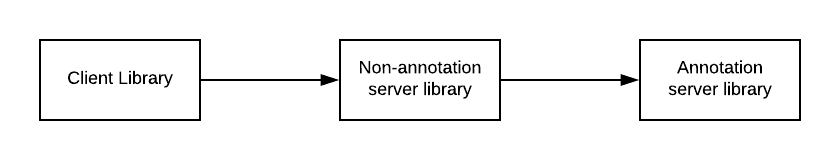
\includegraphics[width=\textwidth]{figures/Transitivity-Annotations.png}
\caption{Example dependency tree involving annotations}
\label{fig:annotation-dependencies}
\end{center}
\end{figure}

\section{Experiment 3: Sensitivity Analysis}
As explained before, we have not been able to obtain the real-world data to understand how the impact of the transitive dependencies behaves, and correlate it with our transitive coupling metrics \texttt{TMIC}, and \texttt{TAC}. Therefore, we cannot know which would be the actual value of the \textit{propagation factor} for these two metrics. Instead, what we do is a sensitivity analysis of the \textit{propagation factor} on these two metrics.

A \textit{Sensitivity Analysis} consists of analyzing how much an input variable affects the output. In this case, the input variable is the \textit{propagation factor}, and the output is the value of the metrics.

\subsection{Experimental set up}

To run this analysis, we have set up a new request in the API of the PoC. This request receives a list of Maven artifacts in a \textit{.txt} file (tab-delimited). The file includes three columns, containing for each artifact, the following information: \textit{group id}, \textit{artifact id}, and \textit{version}.

The first step is to run the dependency model's calculation for each of the dependencies of the artifacts. Then, for each one of the transitive dependencies with coupling, we run the sensitivity analysis. Since the \textit{propagation factor} is a value in the range $(0,1)$, we calculate the value of the metrics incrementing the propagation factor by $0.01$ from $0.01$ to $0.99$.

We run this experiment with a randomly selected subset of the libraries used for the significance experiment. Then, out of the set of dependencies that can be used for the sensitivity analysis, we select a representative subset. This subset is chosen to have dependencies with different distances, and values measured at each distance. The dependencies used for the sensitivity analysis can be found in Table \ref{table:sensitivity-dependencies}.

\begin{table}[ht!]
\begin{center}
\begin{tabularx}{\textwidth}{|X|X|}
\hline
\textbf{Client library} & \textbf{Server library} \\ \hline
org.asynchttpclient async-http-client 2.12.1 & io.netty netty-common 4.1.48.Final \\ \hline
org.asynchttpclient async-http-client 2.12.1 & io.netty netty-buffer 4.1.48.Final \\ \hline
org.easymock easymock 4.2 & org.hamcrest hamcrest-core 1.3 \\ \hline
org.apache.maven maven-project 3.0-alpha-2 & org.codehaus.plexus plexus-classworlds 1.3 \\ \hline
org.springframework.boot\newline spring-boot-autoconfigure 2.3.4.RELEASE & org.springframework\newline spring-core  5.2.9.RELEASE \\ \hline
org.springframework.boot\newline spring-boot-autoconfigure 2.3.4.RELEASE & org.springframework\newline spring-jcl  5.2.9.RELEASE \\ \hline
org.springframework.boot\newline spring-boot-autoconfigure 2.3.4.RELEASE & org.springframework\newline spring-beans  5.2.9.RELEASE \\ \hline
org.eclipse.jetty jetty-server 11.0.0.beta1 & org.eclipse.jetty jetty-util 11.0.0.beta1 \\ \hline
org.asynchttpclient async-http-client 2.12.1 & log4j log4j 1.2.17 \\ \hline
org.alluxio alluxio-core-transport 2.3.0 & com.google.protobuf protobuf-javalite 3.11.0 \\ \hline
fr.inria.gforge.spoon spoon-core 8.2.0 & org.eclipse.platform org.eclipse.osgi 3.16.0 \\ \hline
fr.inria.gforge.spoon spoon-core 8.2.0 & org.eclipse.platform org.eclipse.equinox.preferences 3.8.0 \\ \hline
fr.inria.gforge.spoon spoon-core 8.2.0 & org.eclipse.platform\newline org.eclipse.equinox.common 3.13.0 \\ \hline
com.puppycrawl.tools checkstyle 8.36.2 & log4j log4j 1.2.17 \\ \hline
com.puppycrawl.tools checkstyle 8.36.2 & org.apache.geronimo.specs\newline geronimo-jms 1.1\_spec\_1.0 \\ \hline
\end{tabularx}
\end{center}
\caption{Sensitivity analysis, list of dependencies used}
\label{table:sensitivity-dependencies}
\end{table}

\subsection{Results}
With the data obtained from running the experiment, we calculate the covariance of the metrics \texttt{TMIC} and \texttt{TAC} with the \textit{propagation factor}. The values of the covariance are displayed in Table \ref{table:covariance-sensitivity}.

\begin{table}[ht!]
\begin{center}
\begin{tabular}{|l|l|}
\hline
\textbf{TMIC Covariance} & \textbf{TAC Covariance} \\ \hline
21.39853 & 7.740404 \\ \hline
35.28688 & 4.461675 \\ \hline
0.6733333 & 1.515 \\ \hline
1.431675 & 0.6767 \\ \hline
15.34022 & 2.278392 \\ \hline
5.914392 & 1.01505 \\ \hline
3.535 & 0.9258333 \\ \hline
16.83586 & 4.545 \\ \hline
0.3400333 & 2.014634 \\ \hline
35.94001 & 6.228333 \\ \hline
10.21567 & 0.5870659 \\ \hline
9.179277 & 1.225487 \\ \hline
31.63428 & 1.783189 \\ \hline
1.323955 & 0.674175 \\ \hline
2.916436 & 1.360133 \\ \hline
\end{tabular}
\end{center}
\caption{Covariance of the dependencies used in the sensitivity analysis}
\label{table:covariance-sensitivity}
\end{table}

\unsure{Here, should I add a table with all the coefficients? Or maybe add them to the previous table?}
In addition, we also calculate the \textit{Pearson correlation coefficient}. The values of the correlation range from $0.941282$ to $1$ for \texttt{TMIC}, and from $0.9445726$ to $1$ for \texttt{TAC}. In Figure \ref{correlation-sensitivity}, one can see a scatter plot displaying the correlation between the value of \texttt{TMIC} (upper plot) and \texttt{TAC} (lower plot), and the \textit{propagation factor}. The figure shows the values of the sensitivity analysis done for the client library \textit{fr.inria.gforge.spoon:spoon-core:8.2.0} and the server library \textit{org.eclipse.platform:org.eclipse.osgi:3.16.0}.

\begin{figure}[ht!]
\begin{center}
  \begin{subfigure}[b]{0.7\textwidth}
    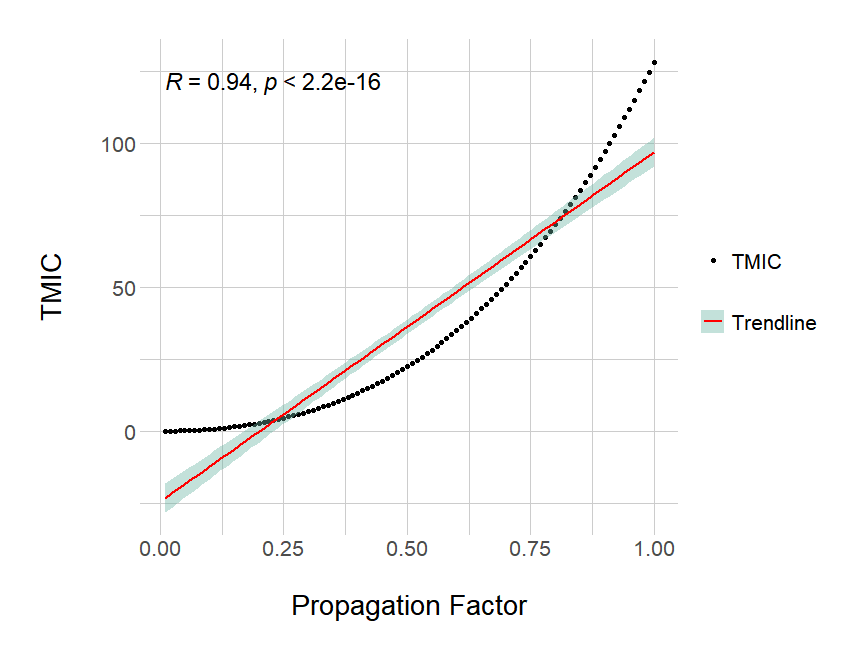
\includegraphics[width=\textwidth]{figures/results/Rplot_spoon-core_eclipse-osgi_TMIC.png}
  \end{subfigure}
  %
  \begin{subfigure}[b]{0.7\textwidth}
    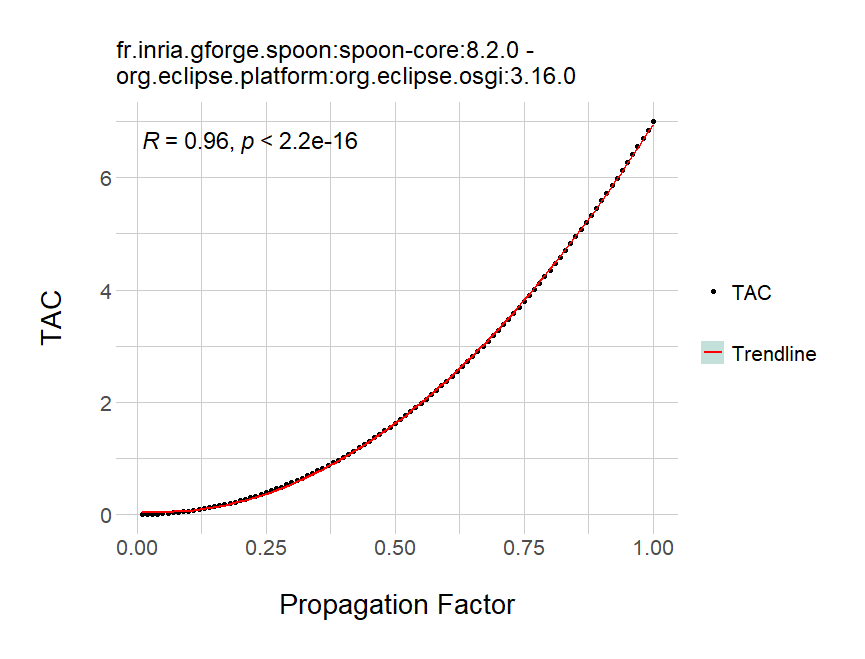
\includegraphics[width=\textwidth]{figures/results/Rplot_spoon-core_eclipse-osgi_TAC.png}
  \end{subfigure}
\caption{Scatter plot sensitivity analysis, correlation \textit{propagation factor} with \texttt{TMIC}, and \texttt{TAC}}
\label{fig:correlation-sensitivity}
\end{center}
\end{figure}

\subsection{Discussion}
The sensitivity analysis results indicate a high sensitivity of the two coupling metrics to the propagation factor since there is a high correlation between these two values, the \textit{Pearson correlation coefficient} is always higher than $0.94$.

\begin{finding}
	The value of the metrics \texttt{TMIC} and \texttt{TAC} is highly sensitive to the value of the \textit{propagation factor}.
	\label{find:high-sensitivity}
\end{finding}

In Table \ref{table:covariance-sensitivity}, we can see that the values of the covariance for \texttt{TMIC} are always greater than those of \texttt{TAC}. This seems to be related to the fact that the values measured for \texttt{TMIC} are greater than those measured for \texttt{TAC}. Also, the cases in which the covariance is greater than $30$ seem to have greater coupling values measured as well. To confirm this intuition, we create a scatter plot to compare the covariance with the sum of the coupling measured at each distance. These plots can be seen in Figure \ref{fig:cov-value-tmic} and \ref{fig:cov-value-tac}, for \texttt{TMIC} and \texttt{TAC} respectively. In these plots, we have added the correlation between the two values, which confirms that the covariance between the \textit{propagation factor} and the value of the metrics is higher when more coupling is measured.

\begin{figure}[ht!]
\begin{center}
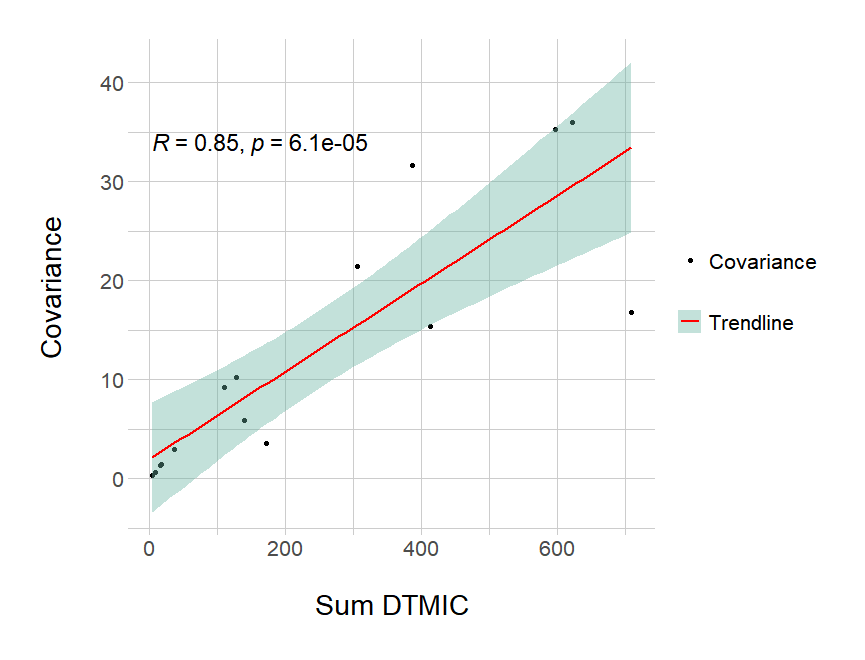
\includegraphics[width=0.7\textwidth]{figures/results/covariance-values-tmic.png}
\caption{Scatter plot, covariance of \textit{propagation factor} and \texttt{TMIC}, and the sumation of the coupling measured at each distance}
\label{fig:cov-value-tmic}
\end{center}
\end{figure}

\begin{figure}[ht!]
\begin{center}
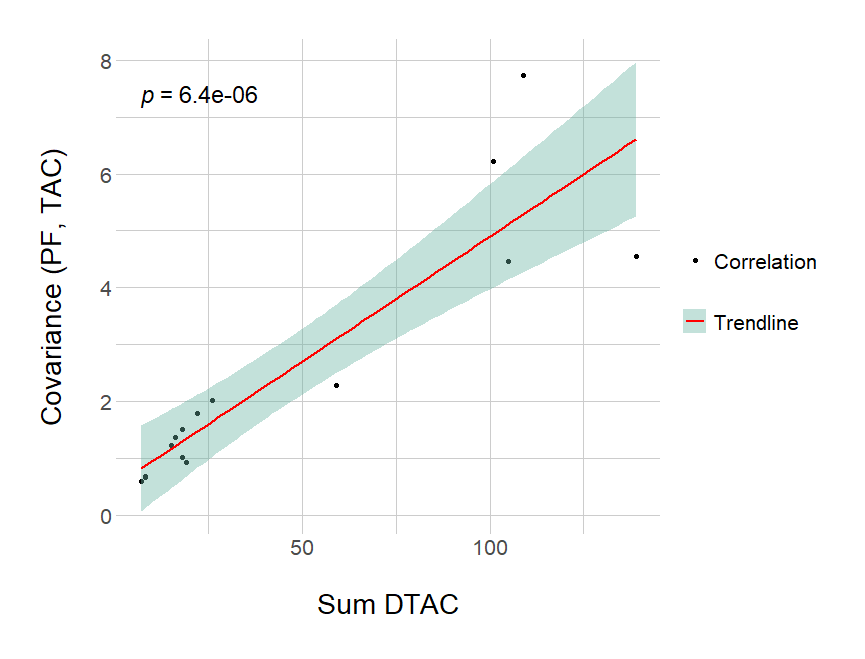
\includegraphics[width=0.7\textwidth]{figures/results/covariance-values-tac.png}
\caption{Scatter plot, covariance of \textit{propagation factor} and \texttt{TAC}, and the sumation of the coupling measured at each distance}
\label{fig:cov-value-tac}
\end{center}
\end{figure}

Finally, in the results of the correlation coefficient between the propagation factor and the metrics, we also observe that the cases with the lowest correlation coefficients tend to be dependencies in which there is more distance between the client library and the server library. To compare the correlation and the distances, we create a scatter plot with the correlation coefficient calculated for the sensitivity analysis and the maximum distance at which coupling is found. The confirmation of this intuition can be found in Figures \ref{fig:cor-dist-tmic} and \ref{fig:cor-dist-tac}.

\begin{figure}[ht!]
\begin{center}
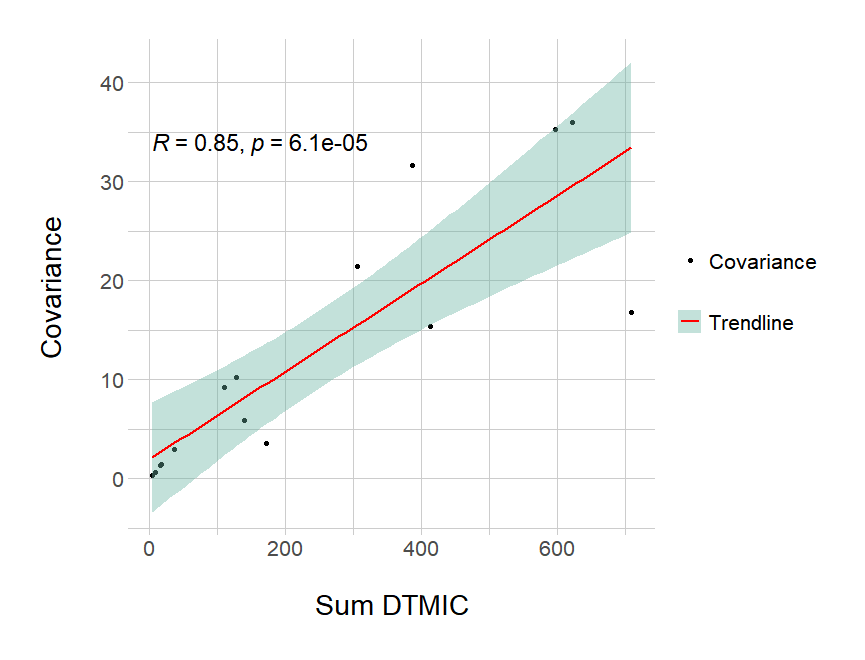
\includegraphics[width=0.7\textwidth]{figures/results/covariance-values-tmic.png}
\caption{Scatter plot, correlation of \textit{propagation factor} and \texttt{TMIC}, and the maximum distance}
\label{fig:cor-dist-tmic}
\end{center}
\end{figure}

\begin{figure}[ht!]
\begin{center}
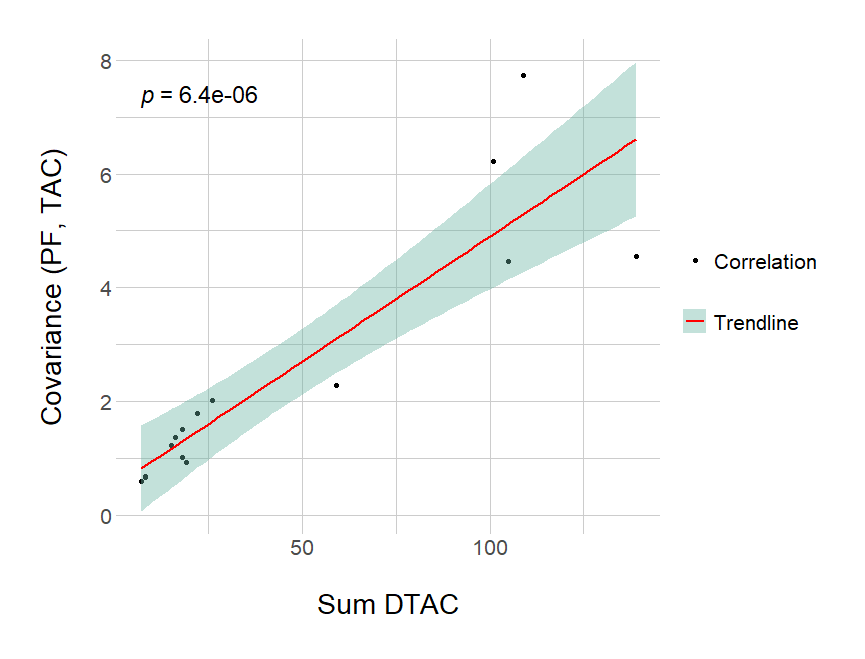
\includegraphics[width=0.7\textwidth]{figures/results/covariance-values-tac.png}
\caption{Scatter plot, correlation of \textit{propagation factor} and \texttt{TAC}, and the maximum distance}
\label{fig:cor-dist-tac}
\end{center}
\end{figure}


\section{Experiment 4: Expert Interviews}
This last experiment has various goals. The main one is to validate the design of the visualization. According to Munzner \cite{Munzner2009}, there are four levels at which this validation can be done:

\begin{enumerate}
  \item Domain Problem and Data Characterization
  \item Operation and Data Type Abstraction
  \item Visual Encoding and Interaction Design
  \item Algorithm Design
\end{enumerate}

In this case, we focus on the third option: Visual Encoding and Interaction Design. To carry out this validation, we designed an \textit{Expert Review} by the means of interviews. In addition, we included questions about the clarity and actionability of the metrics of the model. Therefore, these two aspects of the metrics, which are included in the set of validation criteria defined by Meneely et al. \cite{Meneely2012}, can also be validated.

\subsection{Experimental set up}
The interview consists on 19 questions and a demonstration of the PoC, with two proposed scenarios in which the interviewee uses the tool. The questions are divided in four sections, dividing the interview in a total of five parts:

\begin{enumerate}
  \item \textbf{Demographics:} The questions of this section are related to the interviewee's professional experience and current job.
  \item \textbf{Dependency Management:} In this part, the questions are focused on the interviewee's experience with dependency management and the tools used for this purpose.
  \item \textbf{Demonstration:} The third part is the demonstration of the tool, in which two scenarios are presented to the interviewee. During the scenarios discussion, the interviewee controls the mouse, so the person can interact directly with the tool.
  \item \textbf{Visualizations:} The section after the demonstration contains questions about the tool itself and the designed visualizations.
  \item \textbf{Metrics:} The last section focuses on the designed metrics, the clarity and comprehensibility of these, as well as actionability.
\end{enumerate}

The interviews contain three types of questions: open answer, binary, and scaled from 1 to 5. During every question, even the binary and scaled questions, the interviewee can make comments or discuss the answer. The list of questions contained in the interview, can be found in Table \ref{table:interview-questions}.

\begin{table}[p]
    \begin{center}
    \begin{tabularx}{\textwidth}{|X|l|l|}
    \hline
    Question & Section & Type \\\hline
    \hline
    1.  What is your software development role?  & Demographics & Open answer \\\hline
    2.	How many years of experience do you have as a software developer? & Demographics & Open answer \\\hline
    3.	Which programming language(s) do you usually use in your job? & Demographics & Open answer \\\hline
    4.	Which type of projects do you usually work on? & Demographics & Open answer \\\hline
    \hline
    5.	Do you have experience with dependency management? & Dependency Management & Binary \\\hline
    6.	To what extent is it important to you (or do you try) to have the dependencies up to date? & Dependency Management & Scaled \\\hline
    7.	To what extent is it important to you to monitor the vulnerabilities that your dependencies may be exploiting? & Dependency Management & Scaled \\\hline
    8.	Which tools (if any) do you use for dependency management? & Dependency Management & Open answer \\\hline
    9.	To what extent do you think the tools you used so far are helping you to maintain your dependencies? & Dependency Management & Scaled \\\hline
    \hline
    Scenario 1: You are a new maintainer of the library \textit{org.apache.flink:flink-core}. Since you have not worked in this library's development, you want to see how the dependency tree looks like. What would you look for? & Demonstration & Scenario \\\hline
    Scenario 2: You realize that a library called \textit{kryo} has a new version, which has been announced to contain breaking changes. How likely it would affect your library, and which classes are affected. & Demonstration & Scenario \\\hline
    \hline
    10.	How much do you agree that the tool is useful in the presented scenarios? & Visualizations & Scaled \\\hline
    11.	How much do you agree that managing dependencies would be easier with the presented tool? & Visualizations & Scaled \\\hline
    12.	With your job in mind, which (if any) are the most useful of the visualizations? & Visualizations & Open answer \\\hline
    13.	How much do you agree that the presented tool would be useful in your job? & Visualizations & Scaled \\\hline
    14.	Is there some other visualization or change you would like to see? For which cases do you think it would be useful? & Visualizations & Scaled \\\hline
    \hline
    15.	To what extent do you agree that the metrics are clear and comprehensible? (Answer per metric) & Metrics & Scaled \\\hline
    16.	To what extent do you agree that the metrics are useful in the described scenarios & Metrics & Scaled \\\hline
    17.	To what extent do you agree that the metrics are actionable in the sense that they give you the information you need to make a decision? & Metrics & Scaled \\\hline
    18.	Which (if any) do you think are the most useful of the metrics? Based on the tasks that you usually do in your job. & Metrics & Open answer \\\hline
    19.	Is there some other metric or change that you would like to be added to the model? In which scenarios do you think it could be useful? & Metrics & Open answer \\\hline
    \end{tabularx}
    \end{center}
    \caption{Questions of the interview}
    \label{table:interview-questions}
\end{table}

The interviews are done via \textit{Zoom}\footnote{\url{https://zoom.us/}}. \textit{Zoom} offers the possibility of sharing the control of the mouse with other participants and the option of recording the interview. The interviews are recorded to rewatch it afterward and take notes of the interviewees' answers. Therefore, the interview itself feels more like a normal conversation, and there are no pauses. The control of the mouse was shared with the interviewees to try to use the tool themselves, to get a better idea of how it works and how they would use it.

\subsection{Results}
In this section, we show the answers obtained during the interviews. The results will be discussed in section \ref{sec:discussion-interviews}: the suitability of the visualizations, as well as the clarity and actionability of the metrics.

\subsubsection{Demographics}

The roles of the 15 participants in the interviews include: Software developer, Software engineer, Technology lead, Head of innovation, Head of development, and Head of product. In some of the results, we differentiate between the answers given by developers and managers. In the developers' group, we consider the interviewees who answered with the role of software developer and engineer, and the rest of the interviewees are considered managers. \unsure{I am not sure whether to call this manager or another name. What I mean is that they have tasks that involve software architecture, or reporting, effort estimation. Instead, the developers have programming as their main task}

The years of experience range from 1 to 20, with an average of 7.13. Half of the interviewees have worked in backend development and web services systems. In addition, some of the other types of projects include mobile applications and frontend development. The languages in which the interviewees have experience can be seen in Figure \ref{fig:interview-3}.

\begin{figure}[ht!]
\begin{center}
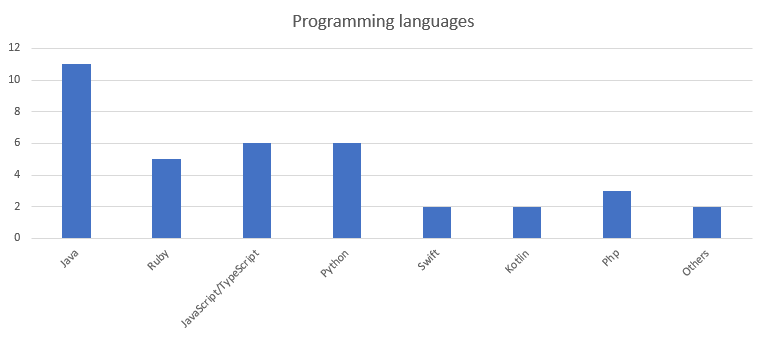
\includegraphics[width=\textwidth]{figures/interview/Question3.png}
\caption{Answers to Question 3 of the interview}
\label{fig:interview-3}
\end{center}
\end{figure}

\subsubsection{Dependency Management}

The 15 interviewees have experience with dependency management. However, some of them indicated that it is not a task that they usually perform in their jobs, but rather in personal projects or time. Figure \ref{fig:interview-6} shows the answers to question 6, regarding the importance of updating the dependencies. The reasons given by the interviewees answering \textit{Neutral} and \textit{Important} for not giving it more importance include: prioritizing the fact that the versions used are compatible, that there are no version incompatibilities with the current version used, and that the version used is stable.

\begin{figure}[ht!]
\begin{center}
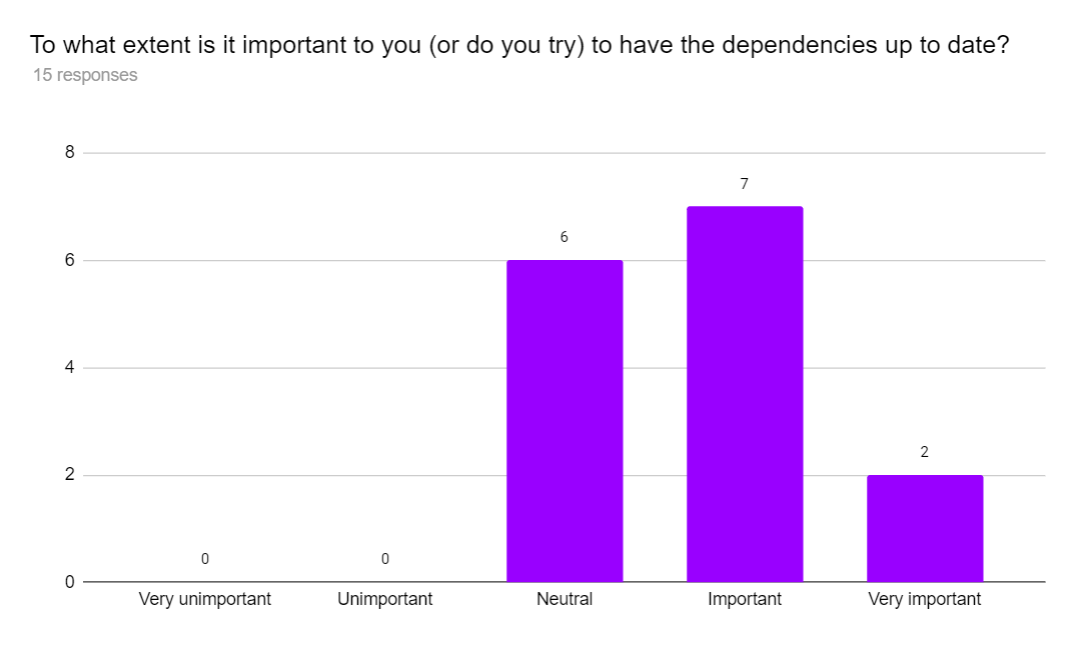
\includegraphics[width=\textwidth]{figures/interview/Question6.png}
\caption{Answers to Question 6 of the interview}
\label{fig:interview-6}
\end{center}
\end{figure}

 Figure \ref{fig:interview-7} the answers to question 7 about the importance of monitoring the dependencies' vulnerabilities. The interviewees which considered that the importance of monitoring the dependencies' vulnerabilities was less than \textit{Very important} reasoned about it. For example, some said that it is something that they do, but not regularly. They just update when there is a new version, to make sure that if a vulnerability has been discovered, the patch is always used. Finally, the last reason depends on the type of dependency that it is, since if it is not a customer-facing dependency, it is not that important.

\begin{figure}[ht!]
\begin{center}
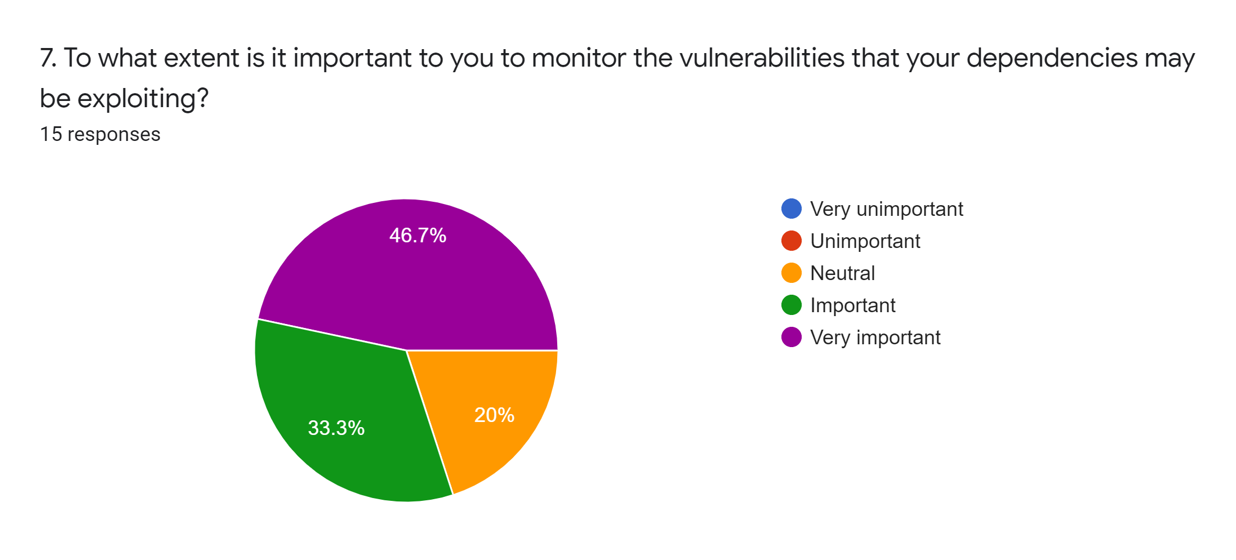
\includegraphics[width=\textwidth]{figures/interview/Question7.png}
\caption{Answers to Question 7 of the interview}
\label{fig:interview-7}
\end{center}
\end{figure}

In Figure \ref{fig:interview-8}, there are the answers to question 8. The interviewees gave more than one answer to the question, but always at least one explicitly included in the figure.

\begin{figure}[ht!]
\begin{center}
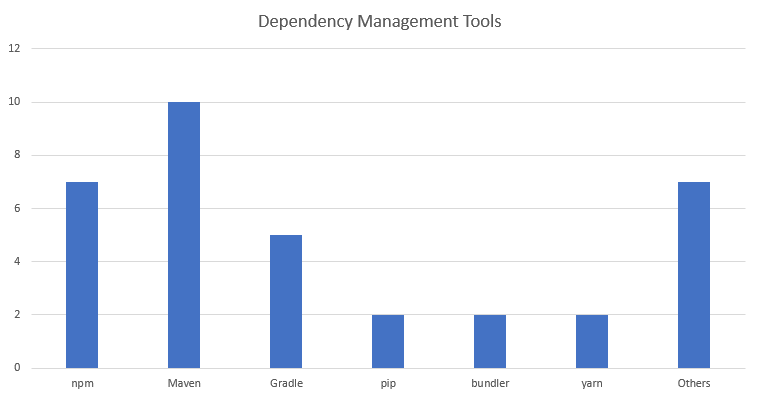
\includegraphics[width=\textwidth]{figures/interview/Question8.png}
\caption{Answers to Question 8 of the interview}
\label{fig:interview-8}
\end{center}
\end{figure}

Finally, the answers to question 9, regarding the how helpul are the tools that the interviewees use for dependency management are. The interviewees that considered the tools to be really helpful (5), compared it to not using any tool. Whilts the interviewees giving lower marks (2-3), considered that features are missing. Mainly, they considered that the basic needs are covered, however some more detailed information about how to manage the dependencies is not there.

\begin{figure}[ht!]
\begin{center}
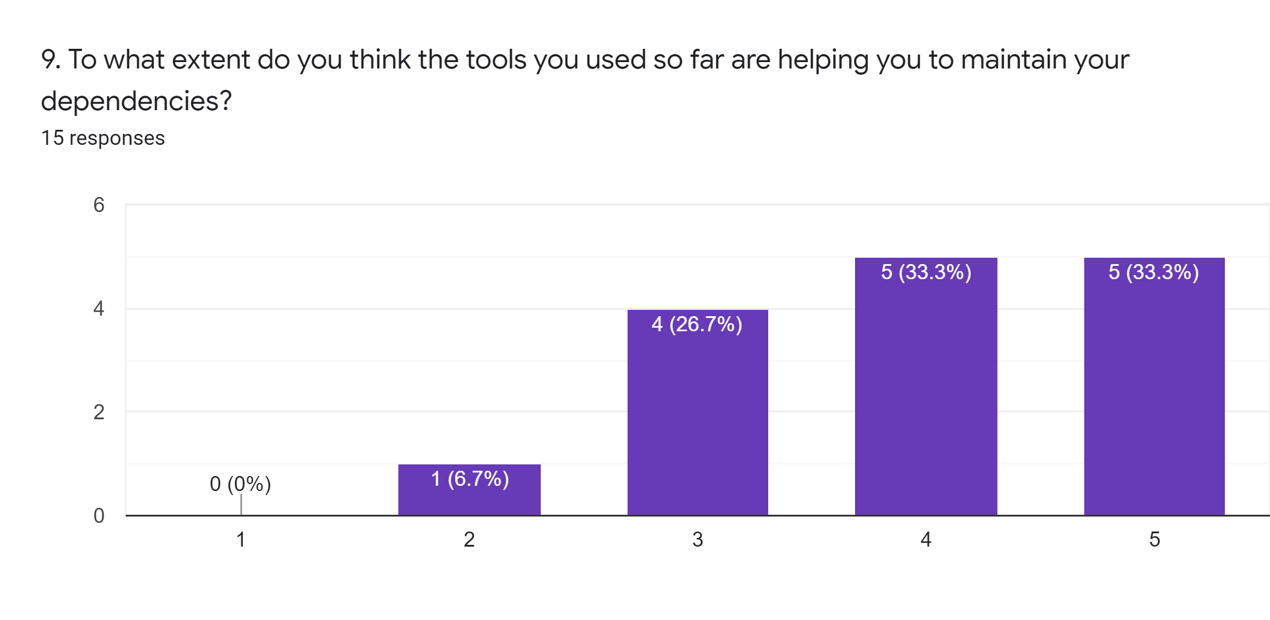
\includegraphics[width=\textwidth]{figures/interview/Question9.png}
\caption{Answers to Question 9 of the interview}
\label{fig:interview-9}
\end{center}
\end{figure}

\subsubsection{Visualizations}

The answers of the interviewees to question 10 about the tool's usefulness are displayed in Figure \ref{fig:interview-10}. Some of the interviewees' reasons for not giving it the maximum grade are the need for improvement in some aspects of both the visualization and the metrics and being useful for some very specific scenarios.

\begin{figure}[ht!]
\begin{center}
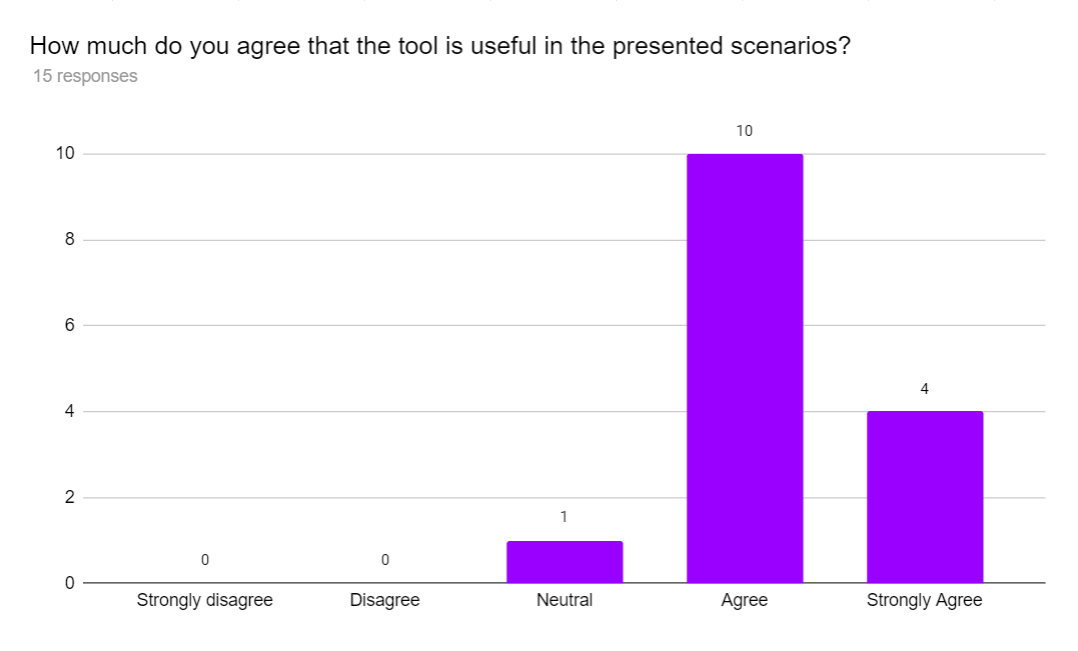
\includegraphics[width=\textwidth]{figures/interview/Question10.png}
\caption{Answers to Question 10 of the interview}
\label{fig:interview-10}
\end{center}
\end{figure}

Figure \ref{fig:interview-11} we can see the results for Question 11. In this case, the interviewees who answered \textit{Disagree} or \textit{Neutral} considered that the tool is meant for some very specific cases, which are not very likely to be needed. The other interviewees agreed that the tool would probably not be used daily, but would make some tasks easier, such as those discussed in the scenarios.

\begin{figure}[ht!]
\begin{center}
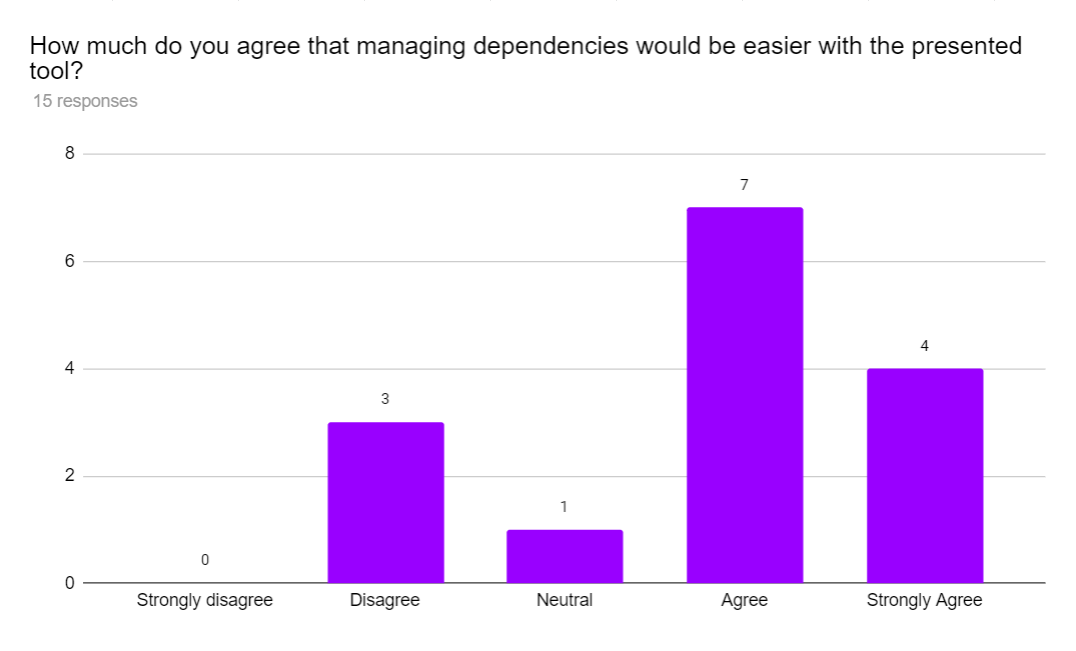
\includegraphics[width=\textwidth]{figures/interview/Question11.png}
\caption{Answers to Question 11 of the interview}
\label{fig:interview-11}
\end{center}
\end{figure}

For Question 12, about which visualizations are most useful, most of the interviews answered with more than one visualization. Table \ref{table:interview-12} summarizes the answers. The $\oplus$ indicates that the interviewee considered that visualization to be the most useful, and the $\odot$ is used when the interviewee said that the visualization was useful but in a clear second position. If the cell is empty, the interviewee did not mention the visualization in the answer.

\begin{table}[ht!]
    \begin{center}
    \begin{tabular}{|c|c|c|}
    \hline
    Tree      & Table     & Barchart \\
    \hline\hline
    $\odot$   & $\oplus$  & ~        \\\hline
    ~	        & ~	        & $\oplus$ \\\hline
    $\oplus$  & ~         & $\oplus$ \\\hline
    $\oplus$	& ~         & ~        \\\hline
    $\oplus$	& $\odot$	  & $\oplus$ \\\hline
    $\oplus$	& ~         & $\odot$  \\\hline
    $\odot$	  & $\oplus$	& ~        \\\hline
    $\oplus$	& $\oplus$	& $\oplus$ \\\hline
    ~	        & ~	        & $\oplus$ \\\hline
    $\odot$	  & $\odot$	  & $\oplus$ \\\hline
    $\oplus$	& $\oplus$	& $\oplus$ \\\hline
    $\oplus$	& ~	        & ~        \\\hline
    $\oplus$	& $\oplus$	& $\oplus$ \\\hline
    $\odot$	  & ~	        & $\oplus$ \\\hline
    $\oplus$	& $\oplus$	& $\oplus$ \\\hline
    \end{tabular}
    \end{center}
    \caption{Answers to Question 12 of the interview}
    \label{table:interview-12}
\end{table}

The answers to Question 13 are shown in Figure \ref{fig:interview-13}. Just as in Question 11, the reason given by the interviewees who answered \textit{Disagree} or \textit{Neutral} are that the tasks for which the tool is useful are not one of the regular tasks in their job.

\begin{figure}[ht!]
\begin{center}
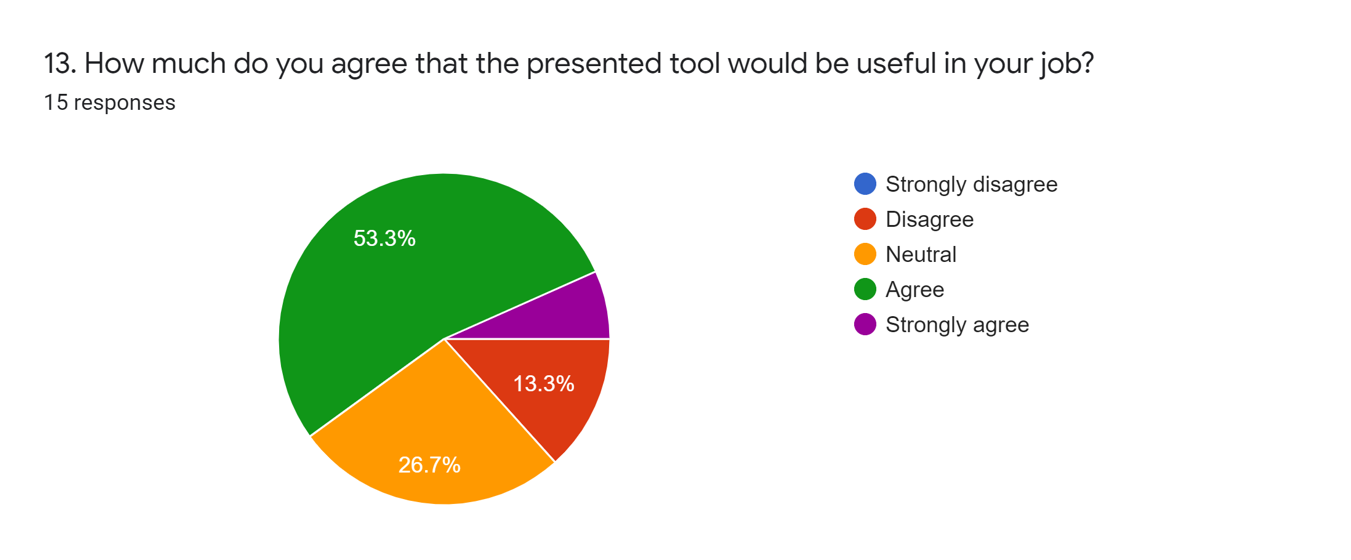
\includegraphics[width=\textwidth]{figures/interview/Question13.png}
\caption{Answers to Question 13 of the interview}
\label{fig:interview-13}
\end{center}
\end{figure}

With Question 14, the interviewees gave their suggestions for improvements to the current visualizations and completely new visualizations. The list of suggestions can be found below:

\begin{itemize}
  \item Add tree visualization at the class level.
  \item List with the classes and methods used from a library.
  \item Add a decision-making model, indicating which actions should be taken.
  \item Visualization to know how much of the system is depending on a library.
  \item Smart visualization displaying some potential problems: the freshness of the dependency, multiple versions of the same library being used.
  \item Color legend in the tree graph.
  \item Tooltip with a description of the metrics of the model.
  \item Display the licenses of the dependencies.
  \item Change the bar chart for a table.
  \item Possibility to move and reorganize the nodes of the tree.
  \item Turn the features into a command interface to be unattended running in the build pipeline.
\end{itemize}

\subsubsection{Metrics}

The answers to question 15 can be found in Figure \ref{fig:interview-15}; for each metric, the number of times an interviewee answered with each number of the options. In addition, Table \ref{table:interview-15} shows the average mark given to each metric, first considering only the marks given by developers, then my managers, and finally, the total average.

\begin{figure}[ht!]
\begin{center}
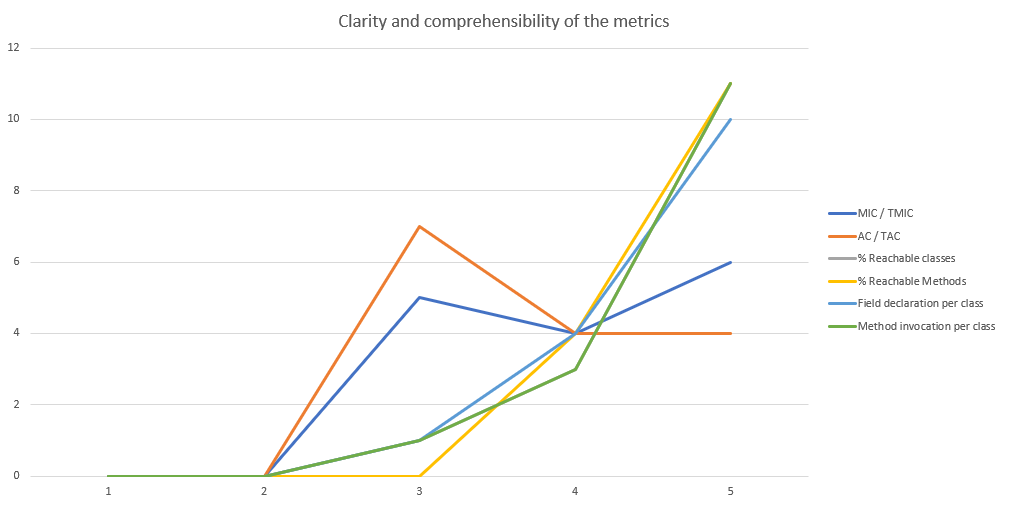
\includegraphics[width=\textwidth]{figures/interview/Question15.png}
\caption{Answers to Question 15 of the interview}
\label{fig:interview-15}
\end{center}
\end{figure}

\begin{table}[ht!]
    \begin{center}
    \begin{tabular}{|l|l|l|l|}
    \hline
    Metric                      & Average developers  & Average managers  & Total Average \\
    \hline
    MIC/TMIC                    & 3.8                 & 4.6               & 4.06 \\
    AC/TAC                      & 3.6                 & 4.2               & 3.8 \\
    \% Reachable classes        & 4.6                 & 4.8               & 4.66 \\
    \% Reachable methods        & 4.8                 & 4.6               & 4.73 \\
    Field declaration per class & 4.8                 & 4.2               & 4.6 \\
    Method invocation per class & 4.8                 & 4.4               & 4.66 \\
    \hline
    \end{tabular}
    \end{center}
    \caption{Results Question 15: Average marks of the metrics, given by developers, managers, and all}
    \label{table:interview-15}
\end{table}

In Figure \ref{fig:interview-16}, there are the answers to question 16 of the interview. The reasons for not giving the metrics the best grade include that it would be more useful if the metrics suggested as missing in question 19 were included. It was also suggested that context is missing for some metrics (e.g., the absolute number of reachable methods and classes, risk assessment for the coupling metrics).

\begin{figure}[ht!]
\begin{center}
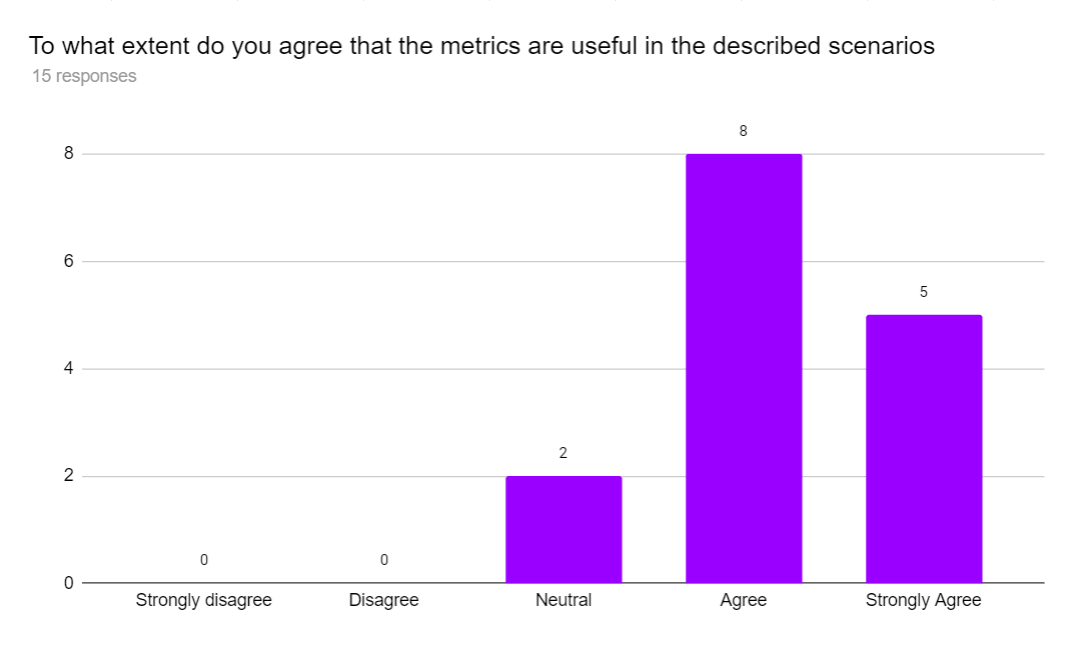
\includegraphics[width=\textwidth]{figures/interview/Question16.png}
\caption{Answers to Question 16 of the interview}
\label{fig:interview-16}
\end{center}
\end{figure}

The answers to question 17 can be found in Figure \ref{fig:interview-17}. The interviewees who gave the grade \textit{Neutral} reasoned that the metrics need some improvements to be trully actionable and that there is information that still can only be found in other places. The interviewees who answered \textit{Agree} suggested that the model's metrics are a good starting point to know which actions to take to start with.

\begin{figure}[ht!]
\begin{center}
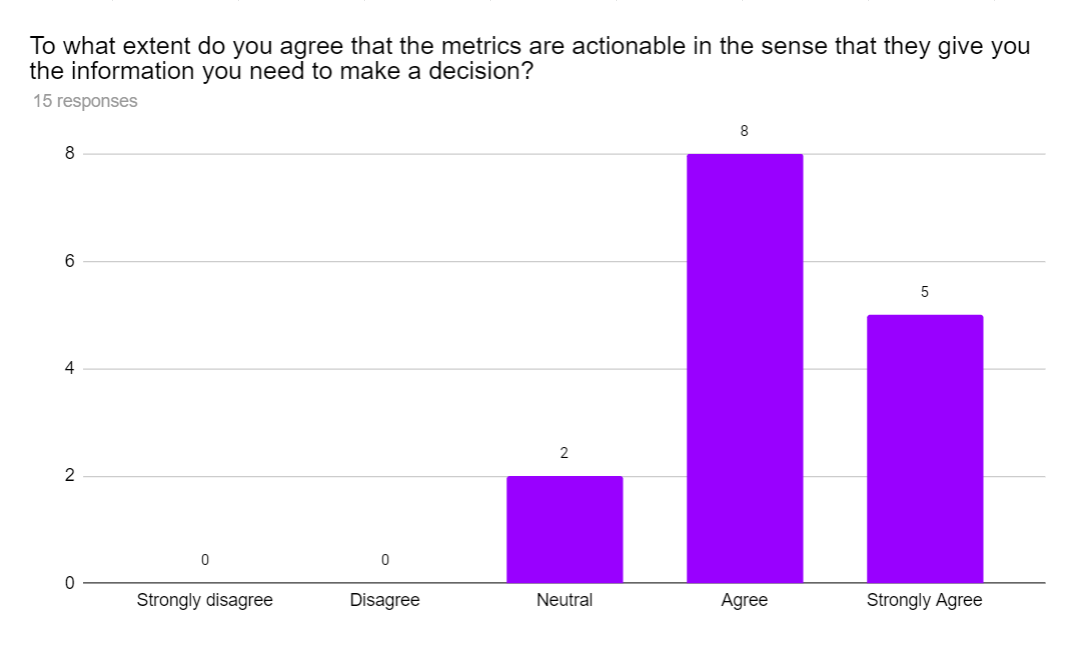
\includegraphics[width=\textwidth]{figures/interview/Question17.png}
\caption{Answers to Question 17 of the interview}
\label{fig:interview-17}
\end{center}
\end{figure}

For question 18, the interviewees answered with which metrics they considered more useful. Their answers can be found in Table \ref{table:interview-18}. As in question 12, a $\oplus$ means that the interviewee mentioned the metric as one of the most useful, $\odot$ is for the metrics mentioned in second place. And finally, if the cell is empty means that the metric was not mentioned. In addition, in the last column, we show the type of role the interviewee had, either development or management.

\begin{table}[ht!]
    \begin{center}
    \begin{tabular}{|c|c|c|c|c|c|l|}
    \hline
    \rot{MIC / TMIC}	& \rot{AC / TAC}	& \rot{\% Reachable classes}	& \rot{\% Reachable Methods}	& \rot{Field declaration per class}	& \rot{Method invocation per class    } & \rot{Role} \\
    \hline\hline
    $\oplus$  & ~	       & $\oplus$	& ~	        & ~	        & ~        & Developer \\\hline
    ~	        & ~	       & $\oplus$	& $\oplus$	& ~	        & ~        & Developer \\\hline
    ~	        & ~	       & $\oplus$	& $\oplus$  & ~	        & ~        & Developer \\\hline
    ~	        & ~	       & ~	      & ~	        & $\odot$	  & $\oplus$ & Developer \\\hline
    ~	        & ~	       & $\oplus$	& $\oplus$	& ~	        & ~        & Developer \\\hline
    ~	        & ~	       & $\oplus$	& $\oplus$	& ~	        & ~        & Developer \\\hline
    $\oplus$	& ~	       & $\oplus$	& $\oplus$	& ~	        & ~        & Manager   \\\hline
    $\oplus$	& ~	       & ~	      & ~	        & ~	        & ~        & Manager   \\\hline
    $\oplus$	& $\oplus$ & $\oplus$	& $\oplus$	& ~	        & ~        & Developer \\\hline
    ~	        & ~	       & $\oplus$	& $\oplus$	& $\oplus$	& $\oplus$ & Developer \\\hline
    $\oplus$	& $\oplus$ & $\oplus$	& $\oplus$	& $\oplus$  & $\oplus$ & Manager   \\\hline
    $\oplus$	& $\oplus$ & ~	      & ~	        & ~	        & ~        & Developer \\\hline
    $\oplus$	& $\oplus$ & ~	      & ~	        & ~	        & ~        & Manager   \\\hline
    ~	        & ~        & $\oplus$ & $\oplus$	& ~         & ~        & Developer \\\hline
    $\oplus$	& ~	       & $\oplus$ & ~	        & ~	        & ~        & Manager   \\\hline
    \end{tabular}
    \end{center}
    \caption{Answers to Question 18 of the interview}
    \label{table:interview-18}
\end{table}

Finally, the suggestions made for improving the current metrics or adding new ones, in the answers of question 19, can be found in the list below:

\begin{itemize}
  \item Min, max, and mean of the coupling metrics.
  \item How much of the client is depending on the server library.
  \item A list of the reachable methods and classes.
  \item The absolute number of reachable methods and classes.
  \item Freshness indicator.
  \item Aggregate of the coupling metrics.
  \item Muber of files of the client using the server library.
  \item Lines of code of the client affected by the dependency.
  \item Code reuse: a combination of the metrics.
\end{itemize}

\subsection{Discussion}
In this section, we discuss the answers to the interviews, divided into sections. First, there is a discussion on the interviewees' general evaluation, according to their role.

We have found a difference in how the interviewees evaluate the model and the visualizations according to whether the interviewee's main focus is development or architecture and analysis.

The developers want more information that can be directly transformed into development actions. For example, they suggested seeing the list of reachable methods of the dependencies, which can answer a vulnerable method is used or not. Another example is the lines of code where the calls to a dependency are made, so the developer can directly go to that line of code to make the necessary changes.

However, the other type of interviewee is interested in more high-level information. One of the suggestions made by several of these interviewees was to create a metric regarding how much of the client library depends on the server library. Also, how widespread the usage is in the client library. These two metrics would be related to the architecture of the system.

Furthermore, there is also an indicator of this difference in their answers to the preferred metric. The coupling metrics are more useful at an architectural level to understand how much a client depends on a server library. In Table \ref{table:interview-18}, we can see that the interviewees with manager role, always mentioned at least \texttt{MIC}/\texttt{TMIC} as the most useful metric. If we compare the average marks of the developers and managers in Table \ref{table:interview-15}, we can see this same difference. The marks given by managers to the coupling metrics are higher than those given by developers.

\subsubsection{Dependency Management}
With the questions answered in the \textit{Dependency Management} section, we know that all the interviewees have experience with this type of task. Also, the interviewees considered it more important to monitor the dependencies' vulnerabilities than the update to the last version (see Figures \ref{fig:interview-6}, and \ref{fig:interview-7}). This is also confirmed by some interviewees' comments, saying that the main reason to update a dependency is to avoid being affected by possible vulnerabilities. \unsure{Should I add a finding of this? Even if it does not relate directly to any of the research questions}

\subsubsection{Visualizations}
When asked about the tool's usefulness, there is a general agreement that the tool is useful in the scenarios discussed during the interview, Figure \ref{fig:interview-10}. There are some negative answers to whether the tool can make dependency management easier. However, most of the comments about these answers are related to the tool being useful for particular cases. Therefore, the negative responses are not associated with the tool, not making the tasks easier.

\begin{finding}
	There is a consensus that the created tool is useful in certain scenarios related to dependency management.
	\label{find:tool-useful}
\end{finding}

In the answers to Question 12, only four interviewees answer only one of the visualizations (see Table \ref{table:interview-12}). Some of the other interviewees also commented that there is value in combining the perspectives in the visualizations. Each visualization has a point of view, which adds to the value of the entire tool. The \textit{Tree} visualization gives an understanding of the hierarchy of the dependencies and where the transitive dependencies come from. The \textit{Table} visualization makes it possible to compare the metrics, and therefore, the degree of dependence. Finally, the \textit{Barchart} gives a more detailed view of the impact of the dependencies in the client library.

\begin{finding}
	It is important to have a different perspective on a system's dependencies in the visualizations to have a complete understanding of the dependency tree.
	\label{find:different-perspectives}
\end{finding}

With the last question about the visualizations, the interviewees suggested some improvements to be made. Certain suggestions are small improvements in terms of interaction with the visualizations, and some other additions to make it easier to use. According to the research method, the next step would be implementing some of these suggestions and doing more interviews. However, due to time limitations, we cannot do these tasks.

Also, some interviewees expressed a need to integrate the different sources of information about dependency management. This data includes vulnerability data, the new versions available of the dependencies, and the licenses of the libraries used. Some related suggestions into making this tool's features into another type of tool are to make it an IDE Plugin and a command interface. Hence, there is a general interest in the tool, but it might be important to consider changing the format in which these are supplied.

\unsure{Should these last two points be made into a finding?}

\subsubsection{Metrics}
Regarding the clarity and comprehensibility of the metrics, the interviewees' average grade for all the metrics is positive, being a 3.8/5, the lowest one, and a 4.73/5 the highest one, as shown in Table \ref{table:interview-15}.

\begin{finding}
	There is a consensus that the metrics defined in this model are clear and comprehensible.
	\label{find:clear-comprehensible}
\end{finding}

The metrics with the lowest grade are the coupling metrics. As confirmed by the comments of the question about the model's actionability, most of the interviewees agreed that the coupling metrics are harder to understand since there is not a clear scale. Therefore, a number gives some information on the dependency itself and how it compares to the rest of dependencies in the tree, but there is no clear meaning that indicates if a certain value is "good" or "bad."

\begin{finding}
	The coupling metrics could be improved with a clear scale or rating evaluation.
	\label{find:coupling-scale}
\end{finding}

The answers to Question 16, about the usefulness of the model, are mainly positive (see Figure \ref{fig:interview-16}). Just as in the visualizations, the interviewees giving the lowest marks reasoned that the need to have such a detailed evaluation of the dependencies is not necessary daily.

\begin{finding}
	The model is useful for dependency management. However, it is not needed for the most common and regular tasks.
	\label{find:model-useful}
\end{finding}

With respect to question 18, regarding which are the most useful metrics in the model, the metrics that got more votes are the coverage metrics, as shown in Table \ref{table:interview-18}. This result is consistent with the answers to Question 15, in which the coverage metrics have two of the highest average scores. Also, just as in the visualizations, some interviewees commented that it is the different perspectives given by each of the metrics making the model more useful.

In the last question of the interviews, we gathered suggestions about the model's metrics and can also be grouped into changes to current metrics and new metrics. One of the main suggestions obtained is to create a combination of the coupling metrics, have a general evaluation, and dive into the detail with the current metrics. The users would then have a general indicator, which can already point them to the dependencies that need a more detailed look.

\begin{finding}
	There is an interest in a general metric indicating the general degree of dependency as a combination of the model's existing metrics.
	\label{find:general-metric}
\end{finding}

We have also obtained some suggestions, which are modifications to the current metrics. For example, having the absolute number of reachable methods or classes and the list of their names. It should be evaluated, which is the need for this information, and in which cases it would be useful.

Finally, one of the suggestions to improve the actionability of the coupling metrics is to create a risk profile of these metrics by evaluating the common values of these metrics and the outliers. This suggestion is further investigated in the following experiment.

\section{Experiment 5: Benchmarking}
One of the main remarks received for the coupling metrics during the interviews is that there is no clear scale for those metrics. Therefore, the metrics' value can be hard to interpret, since there is no indicator of which number is very high or very low.

Hence, we have done a benchmarking of the values of the metrics \texttt{MIC}, \texttt{AC}, \texttt{TMIC}, and \texttt{TAC}. The goal is to understand, which is the distribution of the values and be able to indicate which are the outliers of these metrics.

\subsection{Experimental set up}
To execute this experiment, we have set a new request in the backend of the PoC. This request should contain the path to a \textit{.txt} file, which includes three different columns, tab-delimited. Each row represents a Maven artifact, and for each column it indicates: \textit{group id}, \textit{artifact id}, and \textit{version}.

Then, the calculation of the metrics of the model is performed. For each analyzed dependency, the value of the benchmarked metrics is stored. The result consists on 4 different \textit{.csv} files. The first two contain all the different values of the \texttt{MIC} and \texttt{AC} metrics. The last files represent the values of the transitive coupling metrics, represented in three columns. The first, the dependency id, the second the distance, and the third the value calculated at that distance. Therefore, more than one row might be used to represent the \texttt{TMIC} or \texttt{TAC} of a dependency.

\subsection{Results}

In Figures \ref{fig:MIC-benchmark} and \ref{fig:AC-benchmark}, we show the histograms representing the distribution of the values of \texttt{MIC} and \texttt{AC} respectively.

\begin{figure}[ht!]
\begin{center}
  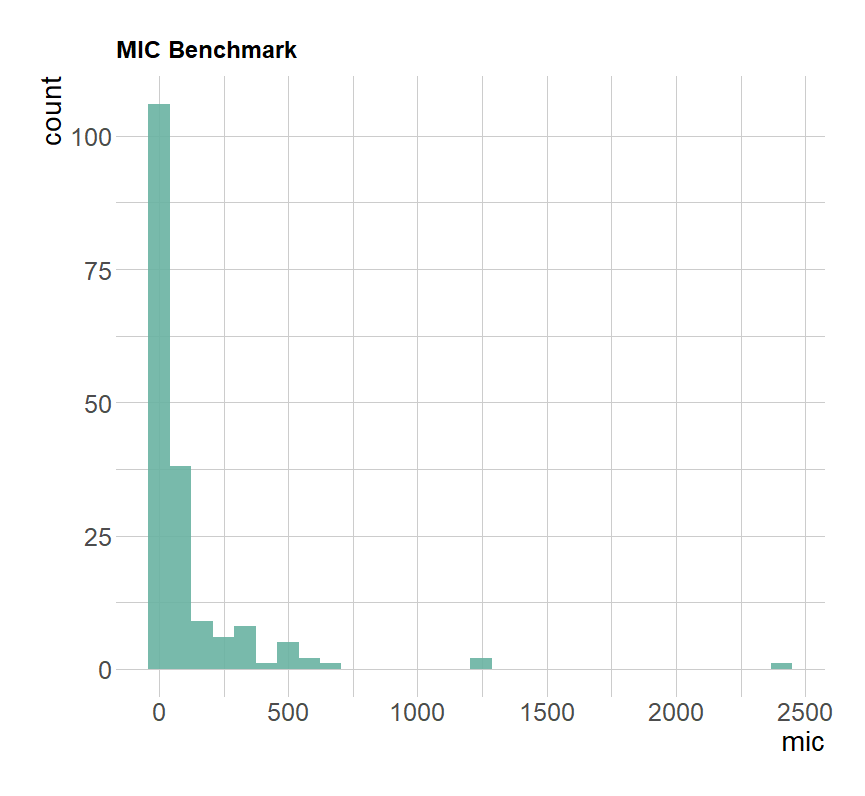
\includegraphics[width=0.7\textwidth]{figures/results/MIC_benchmark.png}
  \caption{Histogram \texttt{MIC} benchmark}
  \label{fig:MIC-benchmark}
\end{center}
\end{figure}

\begin{figure}[ht!]
\begin{center}
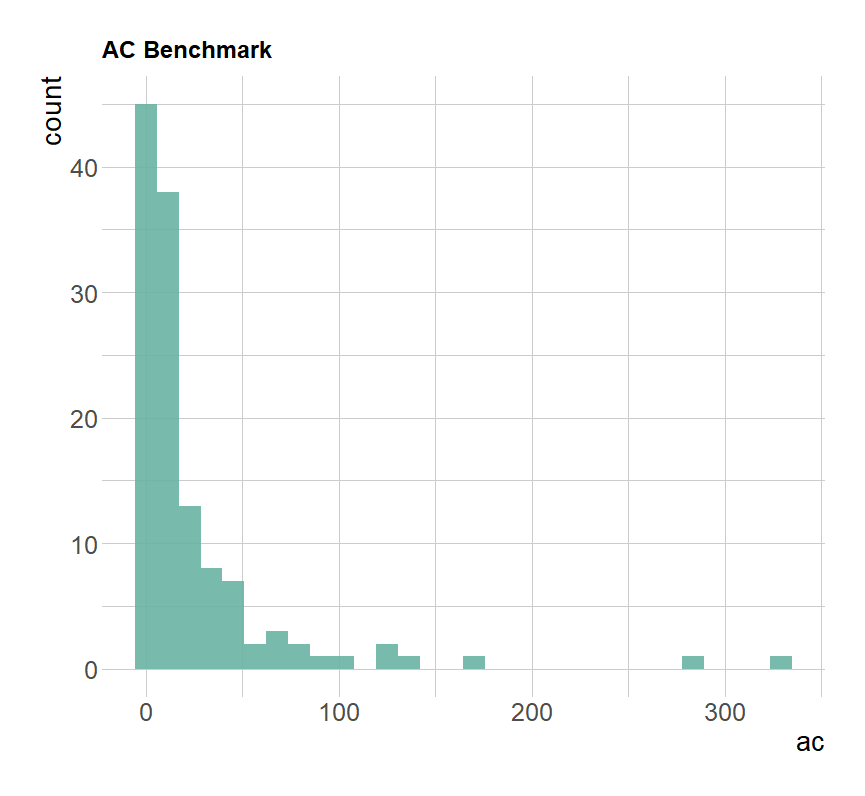
\includegraphics[width=0.7\textwidth]{figures/results/AC_benchmark.png}
\caption{Histogram \texttt{AC} benchmark}
\label{fig:AC-benchmark}
\end{center}
\end{figure}

\newpage
% !TEX root = ..\main.tex
\chapter{Discussion}\label{ch:Discussion}
This chapter discusses the answers to the research questions formulated in this thesis and the process used to obtain these answers and possible threats to validity.

\section{Research Questions}

\subsection{RQ1: How can we measure the degree of code dependency between two software products with a direct dependency?}

To answer this question, we have created the metrics \texttt{MIC} and \texttt{AC}. These metrics measure the coupling between the code of the client and the server library.

\paragraph{RQ1.1: What constitutes a dependency between two products?}

To define what constitutes code dependency, we discuss the meaning of coupling. To define coupling in the scenario of this research question, we use the framework created by Briand et al. \cite{briand1999unified} as described in Section \ref{subsect:defCoupling}. To correctly represent the code dependency scenario between two software products, we adapt the framework. For example, by adding a new aggregation level: the library level.

An important decision in this stage is to define two types of coupling to be considered: the method invocation coupling and aggregation coupling. As discussed previously, these two coupling types could not be sufficient to represent the coupling between two libraries accurately. As mentioned in Section \ref{sec:experiment2}, there are cases in which the two types of coupling metrics measured in this thesis might not be enough. This could be solved by analyzing which types of dependencies could add information about the dependency and design the metric.

\paragraph{RQ1.2: Which metrics can be used to measure the dependency?}

The answer to this question is described in Section \ref{section:defMetrics}. Based on the definition of coupling created to answer the previous question, we formally defined the metrics to measure the degree of code dependency for direct dependencies: Method Invocation Coupling (\texttt{MIC}), and Aggregation Coupling (\texttt{AC}).

\paragraph{RQ1.3: How can the proposed metrics be validated?}

To validate the metrics, we have taken different approaches. First, we have provided proof that both metrics fulfill the five properties of coupling metrics, defined by Briand et al. \cite{briand1996property}, which have been largely used in the literature. Then, from the set of validation criteria for software metrics described by Meneely et al. \cite{Meneely2012}, we selected the actionability and clear definition. Professional developers have conducted the validation of these two criteria.

\subsection{RQ2: How can we measure the degree of code dependency between two software products with a transitive dependency?}

We have adapted the metrics designed for the previous question to measure code dependency of a transitive dependency for this question. The result is the metrics Transitive Method Invocation Coupling \texttt{TMIC} and Transitive Aggregation Coupling \texttt{TAC}. These two metrics consider the distance between the client and the server library, and according to it, apply a \textit{propagation factor}. Due to the libraries between the client library and the server library, the coupling's impact is mitigated. This mitigation modeled with the \textit{propagation factor}. Moreover, the metrics \texttt{TMIC} and \texttt{TAC} use the reachability to measure the coupling. Therefore, only the parts of the server library that are reachable are measured. We have provided a formal definition of both of the coupling metrics for transitive dependencies.

The metrics are validated by proving that they fulfill the five properties of coupling metrics. And as the metrics for direct dependencies, these are included in the expert interviews to evaluate their clarity and actionability.

\subsection{RQ3: How can we measure how much of a dependency is used by a software product?}

This question is answered by creating the coverage metrics: \textit{Percentage of reachable classes} and \textit{percentage of reachable methods}. These two metrics measure how much of a dependency is used by considering the reachable classes and methods compared to the total classes and methods of the dependency. The reachability is measured by considering all possible types of connections between the client and the server. Both of the coverage metrics, are formally defined in Section \ref{sec:coverageMetrics}.

For these metrics, we have conducted a theoretical validation by proving a subset of software metrics' properties that apply to the coverage metrics. Moreover, these metrics were also evaluated by professional developers to validate their actionability and the clarity of their definition.


\subsection{RQ4: How can we visualize the metrics designed to model the software dependencies?}

To visualize the model created during the previous questions, we have added a front-end to the proof-of-concept tool, which contains three visualizations. The first one is a tree graph visualization, which shows the dependency tree's hierarchy, and the unused parts are easily identifiable. Each node of the tree displays the coupling and coverage metrics for the client library and the server library. The second visualization is a table visualization. It shows the data of the server library of each dependency and the metrics measured for each. The table allows the user to filter the dependencies to be displayed and sort according to any values of the table. Finally, there is a third visualization when a dependency is selected. This visualization shows the distribution per class of the server library usage by displaying the usage per class metrics.

This visualization has been validated by conducting expert interviews. The experts agreed that the tool and the visualizations are useful for specific scenarios. Moreover, when asked about the most valuable visualizations, the answers were diverse, indicating no clear favorite. Some of the interviewees said that the combination of the three visualizations is needed. The goal to improve the visualizations is to implement some of the changes suggested by the interviewees and conduct interviews again in a more real-world setup.

When conducting the interviews, we also noticed that there are apparent differences in the opinions of the interviewees according to their roles. Therefore, a study of which perspectives are there, which are the needs of each user, and how to adapt the tool for them.

\section{Proof-of-Concept}

To complete the answers to the questions, we have created the proof-of-concept tool to calculate the metrics of the model for an entire dependency tree, given a client library. The tool is limited to 
- Maven libraries
- Bytecode analysis: missing variables
- Testing libraries
-

\newpage
% !TEX root = ..\main.tex
\chapter{Related Work}\label{ch:RelatedWork}
In this chapter we are going to present the related work to this thesis.

We are going to explain the different topics researched during the literature study part of this project, according to different categories.
For the research activities done during the project, the tool that has been mainly used is \textit{Google Scholar}, as well as \textit{IEEE Xplore}.

\blankl
The papers to be used for this document were selected according to their language (English) and accessibility. Of all the performed searches, we first conducted a selection according to titles and a second filter after reading the abstract and introduction of the papers.
The papers that according to these filters are related and relevant to the topic of this research were completely read and used to create this thesis. For each of the selected papers, the references of the paper were also reviewed.

\section{Dependency management}

As far as we have been able to find, there are no papers that propose a way to measure dependencies between two software products, nor the effort needed to replace one library by another. However, there is a lot of related work in the area of dependency management.

\paragraph{In Dependencies We Trust: How vulnerable are dependencies in software modules? \cite{hejderup2015dependencies}}
In this thesis, Hejderup studies the impact of vulnerabilities in the JavaScript ecosystem. In particular, this research studies the prevalence of known vulnerable modules, the cascading effect of these, and finally the time needed to update libraries to a version without vulnerabilities.
One of the main contributions of this research is the tool used to conduct the experiments to answer the research questions, \texttt{rastogi.js}\footnote{\href{https://github.com/jhejderup/rastogi.js}{https://github.com/jhejderup/rastogi.js}}.

However, in this research the structure used to study the dependencies is not a call-level graph. In the conclusions, Hejderup states: \textit{"On the other hand, reports of a vulnerable dependency are not an immediate sign of a security weakness in a module. There are several factors to this: the module isused in a development environment, the vulnerable functionality of the dependency is not used, or there is a little risk that the vulnerability can be triggered."}. This points out the need for a more detailed analysis of the usage of the dependencies.

\paragraph{Impact Assessment for Vulnerabilities in Open-Source Software Libraries \cite{plate2015impact}}
Plate et al. create a methodology to analyse the impact of a vulnerability in an application that uses the vulnerable library. Their methodology is meant to help assess the need to update the application with a version which does not use the vulnerable version of the library.
The methodology consists on comparing the parts of the library that are used by the application, with the parts updated in the library patch that fixes the vulnerability. The parts of the library used by the application are defined based on dynamic analysis of the application and the bundled libraries.

\paragraph{Vulnerable Open Source Dependencies: Counting Those That Matter \cite{pashchenko2018vulnerable}} % This is the paper that talks about halted dependencies.
In this research, Pashchenko et al. propose a new method to count the dependencies of libraries. This method is used to analyse the dependencies of 200 libraries of the Maven ecosystem. With their method, they differentiate between libraries from the same project and third-party libraries. Furthermore, the dependencies that are not deployed in production (only used for testing or development purposes) are filtered out, since the vulnerabilities of this dependencies do not affect the final product. Furthermore, they consider the special case of halted dependencies, which are the ones that are not being actively developed. Vulnerabilities in halted dependencies suppose an important threat to the software project that depend on these, since the vulnerability is not going to be fixed.

One of the main contributions of this research is a tool implementing the method defined in the paper to detect the vulnerabilities that, according to their definition, matter.

However, Pashchenko et al. do not perform a call-level analysis of the dependencies, since their dependency resolution is based only on the \textit{POM} file of the libraries. Hence, the transitive dependencies that are not really used in the studied library are still counted.

\paragraph{A Comprehensive Study of Bloated Dependencies in the Maven Ecosystem \cite{soto2020comprehensive}}
Soto-Valero et al. conduct a study of the bloated dependencies. The bloated dependencies are those libraries that are included in the compilation of a software product, but that are not really used in the code of the product, neither directly or indirectly. These libraries can be directly included in the dependency declaration file, or included by transitivity or inheritance.

One of the experiments conducted during the research, reported that a 75.1\% of the analyzed dependencies were bloated dependencies. In this experiment Soto-Valero et al. used their tool \texttt{DepClean}\footnote{\href{https://github.com/castor-software/depclean}{https://github.com/castor-software/depclean}} to analyze the dependencies of 9,639 Java artifacts from Maven Central.
The tool \texttt{DepClean} analyses the dependencies of an artifact by creating a call graph of the API members of the libraries involved to define if a dependency is bloated or not.

%\blankl
% decan2018impact --> analysis of how the vulnerabilities in libraries affect the other libraries that depend on these, how the vulnerabilities are fixed, resolved, and updated in the dependent libraries.

% In decan2017empirical Decan et al. studied the evolution of three different package ecosystems, namely npm, CRAN, and RubyGems. The research is focused on their evolution and dependencies, the issues related to dependency updates, and the solutions to these issues. The

% Kikas et al. (kikas2017structure) study three package ecosystems, namely npm, RubyGems and Crates. The authors focus on the structure of the dependency declaration, which affects the way the dependencies are updated. Also, they study the evolution of these ecosystems, and the vulnerability, by studying how many packages would be affected by the removal of a certain package.

\newpage
% !TEX root = ..\main.tex
\chapter{Conclusion}\label{ch:Conclusion}


\printbibliography[heading=bibintoc]
\printglossaries%

% !TEX root = ..\main.tex
\begin{appendices}
\chapter{Data set}\label{appendix:data-set}
The data set used for the experiments \textit{Coupling metrics significance} and \textit{Benchmarking} is displayed in Table \ref{table:data-set}.

\begin{longtable}[h]{|l|l|l|}
  \hline
  Group Id & Artifact Id & Version \\ \hline
  org.apache.flink & flink-core & 1.11.2 \\ \hline
  com.puppycrawl.tools & checkstyle & 8.36.2 \\ \hline
  com.google.auto & auto-common & 0.11 \\ \hline
  edu.stanford.nlp & stanford-corenlp & 4.0.0 \\ \hline
  com.squareup.moshi & moshi-kotlin & 1.10.0 \\ \hline
  org.neo4j & neo4j-collections & 4.1.2 \\ \hline
  org.asynchttpclient & async-http-client & 2.12.1 \\ \hline
  org.alluxio & alluxio-core-transport & 2.3.0 \\ \hline
  com.github.javaparser & javaparser-symbol-solver-logic & 3.15.15 \\ \hline
  io.undertow & undertow-benchmarks & 2.2.0.Final \\ \hline
  org.teavm & teavm-core & 0.6.1 \\ \hline
  com.github.jknack & handlebars-markdown & 4.2.0 \\ \hline
  ma.glasnost.orika & orika-eclipse-tools & 1.5.4 \\ \hline
  fr.inria.gforge.spoon & spoon-core & 8.2.0 \\ \hline
  org.jacop & jacop & 4.7.0 \\ \hline
  com.google.guava & guava & 29.0-jre \\ \hline
  com.fasterxml.jackson.core & jackson-databind & 2.11.2 \\ \hline
  org.clojure & clojure & 1.10.1 \\ \hline
  org.apache.logging.log4j & log4j-core & 2.13.3 \\ \hline
  javax.servlet & javax.servlet-api & 4.0.1 \\ \hline
  org.mockito & mockito-core & 3.5.11 \\ \hline
  org.apache.httpcomponents & httpclient & 4.5.12 \\ \hline
  org.slf4j & slf4j-simple & 1.7.30 \\ \hline
  org.junit.jupiter & junit-jupiter-api & 5.7.0 \\ \hline
  org.slf4j & slf4j-log4j12 & 1.7.30 \\ \hline
  joda-time & joda-time & 2.10.6 \\ \hline
  com.squareup.okhttp3 & okhttp & 4.9.0 \\ \hline
  mysql & mysql-connector-java & 8.0.21 \\ \hline
  org.easymock & easymock & 4.2 \\ \hline
  org.hamcrest & hamcrest-core & 2.2 \\ \hline
  commons-beanutils & commons-beanutils & 1.9.4 \\ \hline
  org.apache.logging.log4j & log4j-slf4j-impl & 2.13.3 \\ \hline
  org.springframework & spring-core & 5.2.9.RELEASE \\ \hline
  org.slf4j & jul-to-slf4j & 2.0.0-alpha1 \\ \hline
  org.eclipse.jetty & jetty-server & 11.0.0.beta1 \\ \hline
  com.sun.xml.bind & jaxb-impl & 3.0.0-M4 \\ \hline
  org.jetbrains.kotlin & kotlin-stdlib & 1.4.10 \\ \hline
  org.apache.maven & maven-project & 3.0-alpha-2 \\ \hline
  org.apache.maven & maven-artifact & 3.6.3 \\ \hline
  org.apache.camel & camel-core & 3.5.0 \\ \hline
  org.slf4j & jcl-over-slf4j & 2.0.0-alpha1 \\ \hline
  org.reflections & reflections & 0.9.12 \\ \hline
  org.apache.ant & ant & 1.10.8 \\ \hline
  xerces & xercesImpl & 2.12.0 \\ \hline
  org.slf4j & log4j-over-slf4j & 2.0.0-alpha1 \\ \hline
  com.sun.xml.bind & jaxb-core & 3.0.0-M4 \\ \hline
  org.scala-js & scalajs-library\_2.12 & 1.2.0 \\ \hline
  commons-logging & commons-logging & 1.2 \\ \hline
  commons-fileupload & commons-fileupload & 1.4 \\ \hline
  org.springframework.boot & spring-boot-autoconfigure & 2.3.4.RELEASE \\ \hline
  org.springframework & spring-jdbc & 5.2.9.RELEASE \\ \hline
  org.springframework & spring-webmvc & 5.2.9.RELEASE \\ \hline
  org.springframework & spring-aop & 5.2.9.RELEASE \\ \hline
  org.springframework & spring-orm & 5.2.9.RELEASE \\ \hline
  org.springframework & spring-tx & 5.2.9.RELEASE \\ \hline
  org.springframework & spring-web & 5.2.9.RELEASE \\ \hline
  org.springframework & spring-beans & 5.2.9.RELEASE \\ \hline
  org.springframework & spring-context & 5.2.9.RELEASE \\ \hline
  org.springframework & spring-context-support & 5.2.9.RELEASE \\ \hline
  com.google.inject & guice & 4.2.3 \\ \hline
  com.google.guava & guava & 29.0-jre \\ \hline
  com.google.code.findbugs & annotations & 3.0.1 \\ \hline
  ch.qos.logback & logback-core & 1.3.0-alpha5 \\ \hline
  ch.qos.logback & logback-classic & 1.3.0-alpha5 \\ \hline
  \caption{List of libraries from Maven Central used in the experiments 2 and 5.}
  \label{table:data-set}
\end{longtable}

\end{appendices}


\end{document}
